\documentclass[12pt,a4paper]{report}

\usepackage[utf8]{inputenc}
\usepackage[T1]{fontenc}
\usepackage{lmodern}
\usepackage[
  top=2.5cm,
  bottom=2.5cm,
  left=3cm,
  right=2.5cm
]{geometry}
\usepackage{setspace}
\onehalfspacing
\usepackage{microtype}

\usepackage{amsmath,amssymb,amsfonts}
\usepackage{graphicx}
\usepackage{booktabs}
\usepackage{longtable}
\usepackage{array}
\usepackage{tabularx}
\usepackage{pdflscape}
\usepackage{caption}
\usepackage{subcaption}
\usepackage{xcolor}
\usepackage{enumitem}
\usepackage[ruled,vlined,linesnumbered]{algorithm2e}
\usepackage{listings}
\usepackage{tikz}
\usetikzlibrary{arrows.meta,positioning,shapes.geometric,calc,fit,backgrounds}
\usepackage{xurl}
\usepackage[
  colorlinks=true,
  linkcolor=blue!65!black,
  citecolor=green!45!black,
  urlcolor=blue!65!black
]{hyperref}
\usepackage[round,sort&compress]{natbib}
\Urlmuskip=0mu plus 1mu
\emergencystretch=2em

\graphicspath{{./}{../../paper/figures/}{../../paper/figures/v2/}{../../grpo_ablation_results/images/}}

\newcommand{\projecttitle}{When Does GRPO Have a Learning Signal?}
\newcommand{\projectsubtitle}{An Empirical Study of Reward Diversity, Structured Outputs, and Reasoning Benchmarks in LLM Post-Training}
\newcommand{\zvf}{\mathrm{ZVF}}
\newcommand{\gu}{\mathrm{GU}}
\newcommand{\fitdiagram}[1]{\resizebox{\textwidth}{!}{\input{#1}}}

\lstset{
  basicstyle=\ttfamily\small,
  breaklines=true,
  frame=single,
  numbers=left,
  numberstyle=\tiny,
  captionpos=b
}

\bibliographystyle{plainnat}

\begin{document}

\hypersetup{pageanchor=false}
\begin{titlepage}
  \centering
  \vspace*{1.2cm}
  {\LARGE\bfseries PES University, Bengaluru}\\[0.35cm]
  {\large Department of Computer Science and Engineering}\\[0.25cm]
  {\large M.Tech in Data Science and Artificial Intelligence}\\[1.8cm]

  \rule{\textwidth}{1.2pt}\\[0.55cm]
  {\Huge\bfseries \projecttitle}\\[0.35cm]
  {\Large \projectsubtitle}\\[0.55cm]
  \rule{\textwidth}{1.2pt}\\[1.4cm]

  {\Large\bfseries Final Capstone Report}\\[1.0cm]

  {\large\bfseries Group 6}\\[0.35cm]
  \begin{tabular}{rl}
    Arvind C R & PES2PGE24DS006\\
    Madhu Kumara L & PES2PGE24DS176\\
    Sandhya Jeyaraj & PES2PGE24DS101\\
    Arumugam Chetty K & PES2PGE24DS022\\
    Dhruva N Murthy & PES2PGE24DS054\\
    Mohammad Rafi & PES2PGE24DS189\\
  \end{tabular}\\[1.0cm]

  {\large\bfseries Project Guides}\\[0.25cm]
  Prof.\ Narayana Darapaneni\\
  Mr.\ Anwesh Reddy Paduri\\[1.0cm]

  \vfill
  {\large April 21, 2026}
\end{titlepage}
\hypersetup{pageanchor=true}

\pagenumbering{roman}

\chapter*{Abstract}
\addcontentsline{toc}{chapter}{Abstract}
This project studies when critic-free reinforcement learning helps post-train language models and when it fails. The central algorithm is Group Relative Policy Optimization (GRPO), a value-free alternative to PPO that normalizes rewards within sampled response groups. We apply GRPO to structured tool-call emission, mathematical reasoning, and code generation, while also comparing against supervised fine-tuning, DPO-style preference training, classical RL baselines, TRL GRPO, and PPO experiments on Modal H100 GPUs. Across the collected evidence, the strongest positive result is not broad reasoning improvement but structured behavior acquisition: after an SFT warm-up, GRPO can sharply improve schema-valid tool-call emission. On held-out mathematical reasoning and semantic code generation, however, improvements are weaker, often statistically uncertain, and highly dependent on model family, instruction tuning, reward variance, and implementation framework.

The final evidence base contains the original Tinker cookbook exercises, team member tool-use, code, math, and keyword experiments, the Tinker and Atropos integration work, the 32-run structural-ceiling ablation campaign, the world-class suite over larger dense and MoE models, Modal PPO comparisons, sensitivity runs over temperature, LoRA rank, and batch size, and held-out or partial evaluations. The main empirical conclusion is that GRPO amplifies a useful prior when the model already produces reward-diverse outputs; it does not reliably create reasoning ability from a weak base model. Zero-Variance Fraction (ZVF) and Gradient Utilization (GU) emerge as practical triage diagnostics for flagging obvious reward-signal collapse or saturation; they are not presented as calibrated predictors of final benchmark performance.

\tableofcontents
\listoffigures
\listoftables
\clearpage
\pagenumbering{arabic}

\chapter{Introduction}
\label{ch:introduction}

Large language models increasingly operate as agents: they parse user intent, call external tools, generate code, and solve multi-step reasoning problems. Supervised fine-tuning can teach these systems to imitate demonstrations, but imitation alone is not enough when the desired behavior depends on verifiable success. Tool calls must be syntactically valid and semantically correct; code must pass tests; mathematical answers must match a ground truth. Reinforcement learning offers a direct way to optimize such behaviors against task feedback.

The project initially explored whether GRPO could improve mathematical reasoning in resource-constrained settings, expanding upon the current literature surrounding RLHF, PPO, DPO, GRPO, PEFT, reasoning benchmarks, and RL infrastructure. This inquiry subsequently evolved into a comprehensive scaling and ablation study over model size, model family, group size, learning rate, and training infrastructure. The final scope encompasses structured tool-call emission, code generation, PPO and TRL baselines, MoE models, and larger frontier checkpoints, offering a broad empirical evaluation of critic-free RL.

GRPO is attractive because it avoids the value model required by PPO. For each prompt, it samples a group of completions, scores them with a reward function, and computes advantages relative to the group's reward distribution. The method is simple and memory-efficient, but the same simplicity exposes a failure mode: when all completions in a group receive the same reward, the standard deviation collapses and the update carries little or no learning signal. This project treats that phenomenon as central rather than incidental.

\section{Research Questions}
\label{sec:research-questions}

The final report addresses five research questions. First, under what conditions does GRPO improve structured tool-call emission? Second, how does GRPO performance change with model scale and instruction tuning on mathematical reasoning? Third, how do GRPO and PPO compare on the same model families and tasks? Fourth, how much of the observed behavior is algorithmic, and how much is explained by framework, reward design, and initialization? Fifth, can ZVF and GU flag failure before expensive training is wasted?

\section{Contributions}
\label{sec:contributions}

This report makes six contributions. It consolidates the literature foundation for RLHF, PPO, DPO, GRPO, PEFT, reasoning benchmarks, and RL infrastructure. It documents a multi-domain experimental campaign covering tool-call schemas, GSM8K, MATH, HumanEval, keyword generation, distillation, and style preference learning. It introduces a practical diagnostic view of GRPO through ZVF and GU. It compares training backends, including Tinker, TRL, Modal H100, and classical RL implementations. It records both positive and negative findings, including structured-output gains, held-out math non-significance, small-model failure, and code-generation instability. Finally, it provides a reproducible report source with TikZ diagrams and a source map for future project handoff.

\section{Thesis Statement and Central Arguments}
\label{sec:central-arguments}

The thesis statement of this report is that critic-free reinforcement learning for LLM post-training is governed less by the nominal algorithm label than by reward variance, base-model sampling competence, and backend implementation. GRPO can refine behavior when the model already samples mixed-quality completions under a reward that differentiates them; it does not reliably create reasoning competence when every sampled completion receives the same sparse reward. Three arguments carry this originality claim and are highlighted here so the reader can track them through the Results and Analysis chapter.

\subsection*{Three central arguments and how they engage the literature}

Three arguments carry the report's main originality claim and are highlighted here so the reader can track them through the Results and Analysis chapter.

\paragraph{A1 --- Mixed-reward sampling condition: GRPO needs non-flat groups.}
\emph{Thesis.} The key precondition for critic-free GRPO under sparse verifiable rewards is not task domain but mixed-group probability: GRPO can only update meaningfully when the base model, group size, and reward function together make non-uniform reward groups likely. Under an i.i.d. binary-reward simplification, the relevant probability is $P(\text{usable group}) = 1 - p_0^{G} - (1-p_0)^{G}$; the familiar $p_0\!>\!1/G$ is only an \emph{expected-one-success heuristic}, not a necessary or sufficient threshold. This argument refines the broad reading of DeepSeek-Math~\citep{shao2024deepseekmath} and DeepSeek-R1~\citep{deepseek2025r1}: GRPO can be a strong reasoning trainer when the starting policy and reward design generate mixed-quality rollouts, but sparse verifier-only cold starts can leave the estimator with no useful ordering signal. It also aligns with zero-variance-prompt and difficulty-selection work~\citep{rlzvp2025,rcgrpo2026,pikus2025hardexamples}, which likewise treats group outcome diversity as central. Four rescue hypotheses follow: increase $G$ (reduces the all-wrong term $(1-p_0)^G$), add SFT warm-up (lifts $p_0$), densify the reward (moves outcomes away from the 0/1 extremes), or curriculum the task. Supporting evidence from tool-use ($0.72\to 0.91$ after SFT warm-up, Sandhya 3B) belongs here because it explains \emph{why} warm-up helps, not because ``SFT before RL'' is itself novel. The held-out GSM8K non-significance ($+1.3$\,pp, $p=0.26$) is the companion validity warning: training-reward improvement is a dynamics metric, not proof of generalisation.

\paragraph{A2 --- ZVF/GU as early compute-triage diagnostic, not a calibrated performance predictor.}
\emph{Thesis.} ZVF and GU convert failed GRPO runs into actionable evidence: high-ZVF/low-reward groups identify cold-start collapse, high-ZVF/high-reward groups identify saturation, and only mixed-reward groups indicate useful rollout compute. The pseudo-prospective validation in §\ref{sec:zvf-results} uses only the first five logged steps of each run to flag final-phase collapse. A fixed rule (mean early ZVF $\geq 0.80$ and mean early reward $\leq 0.05$) catches both collapsed runs with zero false positives on 22 de-duplicated runs (TP $=2$, FP $=0$, FN $=0$), but the positive failure count is only two. The continuous-ranking version fails honestly: early ZVF versus late reward has Spearman $\rho=-0.16$, and adding early ZVF to early reward changes leave-one-run-out $R^{2}$ only from $0.885$ to $0.888$. \textbf{Therefore ZVF is a cheap collapse/saturation triage alarm in this corpus, not a calibrated performance predictor.} This argument challenges reward-curve-only reporting in RLHF/RLVR papers---a rising curve can reflect learning, reward hacking, saturation, or parser exploitation---and extends recent GRPO theory that characterises the group-relative gradient as a $U$-statistic with known finite-sample and group-size properties~\citep{zhou2026demystify} by translating its variance behaviour into an experimenter-facing stop/redesign rule. It is complementary to RL-ZVP~\citep{rlzvp2025}, which argues that zero-variance prompts can still be useful if handled specially; our claim is the operational counterpart under standard GRPO.

\paragraph{A3 --- Framework and model family are part of the experimental treatment, not implementation details.}
\emph{Thesis.} In LLM post-training, PPO/GRPO/DPO labels are not complete treatments; algorithm comparisons require backend, model-family, reward, and evaluation controls, because the recorded winner can reverse across otherwise plausible setups. In the recorded comparisons, Qwen3-8B favors GRPO on last-10 reward ($0.344$ vs.\ PPO $0.225$), while Llama-3.1-8B-Instruct favors PPO ($0.975$ vs.\ GRPO $0.844$). The reversal, not the individual direction, is the finding. Because this evidence is not a fully crossed factorial design, the claim is deliberately \emph{methodological rather than causal}: we do not say ``framework caused the reversal.'' We say the reversal shows that model family and backend must be controlled before making algorithm-level claims. This argument \emph{challenges} the prevailing algorithm-comparison style in RLHF/RLVR work, where PPO~\citep{schulman2017proximal}, DPO~\citep{rafailov2024direct}, and GRPO~\citep{shao2024deepseekmath} are described as self-contained methods, and it \emph{extends} Henderson et al.'s classical deep-RL reproducibility critique~\citep{henderson2018deep} from Atari/MuJoCo into LLM post-training: even the same nominal algorithm can reverse rank depending on model family and training stack.

\section{Report Organization}
\label{sec:report-organization}

The report is organized to separate background, design, evidence, interpretation, and audit material. Chapter~\ref{ch:literature-survey} establishes the RLHF, PPO, DPO, GRPO, PEFT, reasoning-benchmark, and infrastructure context. Chapter~\ref{ch:experimental-design} explains why the project uses a multi-axis design rather than a single benchmark leaderboard, and Sections~\ref{sec:grpo-loop}--\ref{sec:claim-evidence-audit} define the training loop, diagnostics, backends, and claim-to-evidence audit used to interpret the runs. Chapter~\ref{ch:experiment-inventory} catalogs the experiment families and explains how individual runs are read. Chapter~\ref{ch:results} reports the empirical verdicts. Chapter~\ref{ch:discussion} interprets those verdicts as design rules for future critic-free RL studies. Chapter~\ref{ch:limitations} states the threats to validity, and Chapter~\ref{ch:conclusion} closes with the practical conclusion and future work. The appendices provide summary tables and artifact locations for independent inspection.

\chapter{Literature Survey}
\label{ch:literature-survey}


\section{Reinforcement Learning from Human Feedback}
\label{sec:rlhf}

The core challenge in deploying large language models is the misalignment between the pretraining objective---predicting the next token on internet text---and the downstream goal of generating outputs that are helpful, honest, and harmless. Reinforcement Learning from Human Feedback (RLHF) emerged as the dominant paradigm for bridging this gap, establishing a systematic pipeline that transforms raw human preference judgments into a training signal capable of steering model behavior. This section traces the intellectual lineage of RLHF, formalizes its three-stage pipeline, and examines the limitations that have motivated subsequent alternatives.

\subsection{Origins and Early Work}

The idea of learning reward functions from human preferences, rather than hand-engineering them, predates the modern LLM era. \cite{christiano2017deep} proposed a framework for \emph{deep reinforcement learning from human preferences}, demonstrating that a reward model trained on pairwise comparisons of trajectory segments could guide an RL agent to solve complex tasks---including Atari games and simulated robot locomotion---without access to the ground-truth reward function. Critically, their approach required human feedback on less than one percent of the agent's total interactions with the environment, making human oversight practically feasible. The reward model was trained by presenting non-expert humans with pairs of short trajectory clips and asking which exhibited more desirable behavior; the resulting learned reward was then optimized via standard policy gradient methods. This work established two foundational principles that would carry forward into the language domain: (i)~pairwise comparisons are a more reliable and cognitively simpler annotation format than absolute scalar ratings, and (ii)~a learned reward model can serve as a proxy objective that decouples the expensive human evaluation from the iterative policy optimization loop.

The transition from simulated environments to natural language was pioneered by \cite{ziegler2019finetuning}, who applied reward learning to fine-tune language models on four tasks: stylistic text continuation (positive sentiment and physically descriptive language) and abstractive summarization on the TL;DR and CNN/DailyMail datasets. Using a pretrained language model as the initial policy, they trained a reward model on approximately 60,000 human comparisons and optimized the policy with Proximal Policy Optimization (PPO)~\cite{schulman2017ppo}. A key technical contribution was the introduction of a Kullback--Leibler (KL) divergence penalty between the learned policy and the original supervised model, which prevented the policy from deviating too far from the pretrained distribution---a regularization mechanism that would become standard in all subsequent RLHF work.

\cite{stiennon2020learning} scaled this approach substantially, applying it to the Reddit TL;DR summarization task with models up to 6.7 billion parameters. They collected a high-quality dataset of 64,832 human comparisons between summaries and demonstrated that policies trained with human feedback significantly outperformed supervised learning baselines---even those with ten times more parameters. Their 6.7B human feedback model produced summaries that human evaluators preferred over the original human-written reference summaries in the dataset. Perhaps most strikingly, the models transferred effectively to out-of-distribution news summarization on CNN/DailyMail without any domain-specific fine-tuning. This work also provided early empirical evidence of \emph{reward over-optimization}: as the policy was optimized more aggressively against the reward model (by reducing the KL penalty coefficient $\beta$), true human preference scores initially improved but eventually degraded, revealing that the reward model's predictions became anti-correlated with genuine quality under heavy optimization.

\subsection{The Three-Stage RLHF Pipeline}

The work of \cite{ouyang2022instructgpt} consolidated and scaled the preceding research into the now-canonical three-stage RLHF pipeline, applying it to align GPT-3 across a broad distribution of real-world user instructions. The resulting system, \textbf{InstructGPT}, became the methodological foundation for ChatGPT and established RLHF as the dominant post-training paradigm for large language models.

\paragraph{Stage 1: Supervised Fine-Tuning (SFT).}
The pipeline begins with supervised fine-tuning of a pretrained language model on a dataset of high-quality demonstrations. In the InstructGPT setting, a team of 40 human contractors wrote demonstrations of desired model behavior for a diverse set of prompts---encompassing generation, open-ended question answering, brainstorming, chat, rewriting, summarization, and classification tasks. A pretrained GPT-3 model was then fine-tuned on approximately 13,000 such demonstration prompts using standard maximum likelihood estimation. The resulting SFT model serves a dual purpose: it provides a strong initialization for the RL policy and establishes a reference distribution against which policy divergence is subsequently penalized.

\paragraph{Stage 2: Reward Model Training.}
The second stage trains a scalar reward model that serves as a proxy for human judgment. Starting from the SFT model with its final unembedding layer replaced by a randomly initialized linear projection head, the reward model is trained to predict which of two candidate completions a human annotator would prefer for a given prompt. \cite{ouyang2022instructgpt} employed a 6B parameter reward model, finding that 175B reward models exhibited training instability.

The reward model is trained under the \textbf{Bradley--Terry} pairwise comparison framework. Given a prompt $x$ and a pair of completions where $y_w$ is preferred over $y_l$ by a human annotator, the probability that $y_w$ is preferred is modeled as:
\begin{equation}
    P(y_w \succ y_l \mid x) = \sigma\!\bigl(r_\theta(x, y_w) - r_\theta(x, y_l)\bigr),
\end{equation}
where $r_\theta(x, y)$ is the scalar reward assigned by the model with parameters $\theta$, and $\sigma(\cdot)$ denotes the logistic sigmoid function. The corresponding training loss is the negative log-likelihood of the observed preferences:
\begin{equation}
    \mathcal{L}_{\text{RM}}(\theta) = -\frac{1}{\binom{K}{2}} \, \mathbb{E}_{(x, y_w, y_l) \sim \mathcal{D}} \Bigl[\log \sigma\!\bigl(r_\theta(x, y_w) - r_\theta(x, y_l)\bigr)\Bigr],
    \label{eq:rm_loss}
\end{equation}
where $\mathcal{D}$ is the dataset of human comparisons and $K$ is the number of candidate responses ranked per prompt. A key efficiency innovation in InstructGPT was presenting labelers with $K \in \{4, \ldots, 9\}$ responses to rank simultaneously, yielding $\binom{K}{2}$ pairwise comparisons per prompt. All comparisons from a single prompt were processed as a single batch element, requiring only one forward pass per completion rather than $\binom{K}{2}$ passes, which both improved computational efficiency and mitigated overfitting caused by the high correlation among comparisons derived from the same ranking task. The reward model outputs were normalized via a bias term so that labeler demonstrations achieved a mean reward of zero before the RL stage.

\paragraph{Stage 3: Reinforcement Learning with PPO.}
In the final stage, the SFT model is fine-tuned as an RL policy to maximize the learned reward signal using Proximal Policy Optimization~\cite{schulman2017ppo}. The environment is formulated as a bandit problem: a prompt $x$ is sampled from the dataset, the policy $\pi_\phi^{\text{RL}}$ generates a response $y$, the reward model assigns a scalar score, and the episode terminates. Each token generation step constitutes an action in the sequential decision process.

To prevent the policy from exploiting imperfections in the reward model---a phenomenon known as \emph{reward hacking}---a per-token KL divergence penalty is added to the reward, constraining the RL policy to remain close to the reference SFT distribution. The augmented objective takes the form:
\begin{equation}
    \mathcal{J}(\phi) = \mathbb{E}_{(x, y) \sim \pi_\phi^{\text{RL}}} \Bigl[r_\theta(x, y) - \beta \, \text{KL}\!\bigl(\pi_\phi^{\text{RL}}(\cdot \mid x) \,\|\, \pi^{\text{SFT}}(\cdot \mid x)\bigr)\Bigr],
    \label{eq:rlhf_objective}
\end{equation}
where $\beta$ controls the strength of the KL penalty. In practice, the KL divergence is computed at the token level as $\sum_t \log \frac{\pi_\phi^{\text{RL}}(y_t \mid x, y_{<t})}{\pi^{\text{SFT}}(y_t \mid x, y_{<t})}$ and subtracted from the reward at each step. The KL penalty serves a dual purpose: it acts as an entropy bonus that encourages exploration and prevents mode collapse, and it constrains the policy to the support of the reward model's training distribution, limiting the scope for reward hacking.

InstructGPT further introduced the \textbf{PPO-ptx} variant, which mixed RL gradients with pretraining gradients on the original language modeling distribution to mitigate performance regressions on standard NLP benchmarks---an instance of the so-called ``alignment tax.'' The combined objective appends a term $\gamma \, \mathbb{E}_{x \sim \mathcal{D}_{\text{pretrain}}}[\log \pi_\phi^{\text{RL}}(x)]$ to Equation~\ref{eq:rlhf_objective}, where $\gamma$ controls the weight of the pretraining loss.

\subsection{InstructGPT: Results and Significance}

The results of \cite{ouyang2022instructgpt} provided compelling evidence for the effectiveness of RLHF at scale. Models were trained at three sizes---1.3B, 6B, and 175B parameters---all using the GPT-3 architecture. The headline finding was striking: \emph{the 1.3B parameter InstructGPT model was preferred by human evaluators over the 175B parameter GPT-3}, despite having more than 100$\times$ fewer parameters. The 175B InstructGPT model was preferred over the 175B GPT-3 baseline 85\% of the time. Beyond raw preference, InstructGPT demonstrated concrete improvements across multiple alignment dimensions. On the TruthfulQA benchmark, InstructGPT generated truthful and informative answers approximately twice as often as GPT-3. Hallucination rates on closed-domain tasks dropped from 41\% to 21\%. Toxic output generation was reduced by approximately 25\% when the model was prompted to be respectful.

These results demonstrated that alignment through human feedback can be far more sample-efficient than scaling model parameters alone. A relatively modest amount of human feedback data---approximately 33,000 comparison prompts for reward model training and 31,000 prompts for PPO---was sufficient to produce dramatic behavioral improvements, suggesting that the \emph{quality} of the training signal matters as much as, or more than, the \emph{quantity} of pretraining compute.

\subsection{Limitations of the Standard RLHF Pipeline}

Despite its empirical success, the standard RLHF pipeline introduces several significant challenges that have motivated subsequent research into simpler alternatives.

\paragraph{Computational Complexity.}
The full RLHF pipeline requires maintaining up to four models simultaneously in GPU memory during the PPO training phase: (i)~the \emph{policy model} being optimized, (ii)~the \emph{reference model} (a frozen copy of the SFT model) for computing the KL penalty, (iii)~the \emph{reward model} for scoring generated completions, and (iv)~the \emph{value/critic model} used by PPO to estimate advantages. For large-scale models, this quadrupling of memory requirements imposes severe infrastructure constraints. \cite{stiennon2020learning} noted the necessity of using completely separate parameters for the policy and value networks to prevent value function updates from destabilizing the pretrained policy, further increasing the memory footprint.

\paragraph{Training Instability.}
PPO-based RLHF training is notoriously sensitive to hyperparameters, including the KL penalty coefficient $\beta$, the PPO clipping ratio, learning rates, and the number of PPO epochs per batch. The interplay between the reward model, the evolving policy, and the value function creates a complex optimization landscape where small perturbations can lead to training collapse or mode collapse. \cite{ouyang2022instructgpt} themselves reported that 175B reward model training was unstable, necessitating the use of a smaller 6B reward model even when training 175B policies.

\paragraph{Reward Hacking and Over-Optimization.}
The reward model is a learned proxy that imperfectly captures the true distribution of human preferences. As the policy is optimized against this proxy, it inevitably discovers outputs that achieve high reward model scores without corresponding improvements in genuine quality---a failure mode known as \emph{reward hacking} or \emph{Goodhart's Law} applied to learned objectives. \cite{stiennon2020learning} provided direct empirical evidence of this phenomenon: as the KL penalty was reduced and the policy optimized more aggressively, reward model scores continued to increase while actual human preference scores first rose and then declined, eventually becoming anti-correlated with the proxy reward. The KL penalty mitigates but does not eliminate this fundamental tension between proxy optimization and true objective alignment.

\paragraph{Human Annotation Bottleneck.}
The pipeline depends critically on the quality, consistency, and scale of human preference annotations. \cite{ouyang2022instructgpt} employed 40 carefully screened contractors, invested in detailed instructions and ongoing calibration, and achieved inter-annotator agreement rates of approximately 73\%. Nevertheless, preference annotations are inherently subjective, expensive to collect at scale, and can encode the biases of the specific annotator pool. The annotation process creates a bottleneck that limits the iteration speed of the overall training pipeline.

\vspace{0.5em}
\noindent These limitations---particularly the computational overhead of maintaining four models and the fragility of PPO-based optimization---have driven the development of alternative approaches. Direct Preference Optimization (DPO) eliminates the reward model entirely by deriving a closed-form policy objective from the same Bradley--Terry preference framework, while Group Relative Policy Optimization (GRPO) replaces the critic model with group-based advantage estimation, reducing the memory footprint while retaining the benefits of RL-based training. These methods, which form the core focus of this work, are discussed in Sections~\ref{sec:dpo} and~\ref{sec:grpo}.

\subsection{Proximal Policy Optimization for Language Models}
\label{sec:ppo}

Proximal Policy Optimization (PPO), introduced by \cite{schulman2017ppo}, has become the dominant reinforcement learning algorithm for aligning large language models with human preferences. PPO belongs to the family of policy gradient methods and was originally designed for continuous control and game-playing tasks. Its adoption as the RL backbone of RLHF---most notably in InstructGPT \cite{ouyang2022instructgpt}---established the standard pipeline for post-training alignment of LLMs. This section presents the PPO algorithm in its general form, describes its adaptation to the language modeling setting, and discusses the practical challenges that motivate the search for simpler alternatives.

\subsubsection{The PPO Algorithm}

Policy gradient methods optimize a parameterized policy $\pi_\theta$ by ascending the gradient of an expected return objective. The vanilla policy gradient estimator takes the form
\begin{equation}
    \hat{g} = \hat{\mathbb{E}}_t \left[ \nabla_\theta \log \pi_\theta(a_t \mid s_t) \, \hat{A}_t \right],
\end{equation}
where $\hat{A}_t$ is an estimator of the advantage function at timestep $t$. A known limitation of this estimator is that performing multiple gradient steps on the same batch of data leads to destructively large policy updates, since the objective is only a valid local approximation of the true performance measure.

Trust Region Policy Optimization (TRPO) addressed this instability by maximizing a surrogate objective subject to a constraint on the KL divergence between successive policies. PPO retains the benefits of trust-region methods while eliminating the need for constrained optimization. The key idea is to define a \emph{clipped surrogate objective} that automatically penalizes policy updates that move the probability ratio too far from unity.

Let $r_t(\theta)$ denote the probability ratio between the current and old policies:
\begin{equation}
    r_t(\theta) = \frac{\pi_\theta(a_t \mid s_t)}{\pi_{\theta_{\text{old}}}(a_t \mid s_t)}.
\end{equation}
The clipped surrogate objective is then defined as
\begin{equation}
    \label{eq:ppo_clip}
    L^{\text{CLIP}}(\theta) = \hat{\mathbb{E}}_t \left[ \min\!\Big( r_t(\theta) \, \hat{A}_t, \;\; \text{clip}\!\big(r_t(\theta),\, 1-\epsilon,\, 1+\epsilon\big) \, \hat{A}_t \Big) \right],
\end{equation}
where $\epsilon$ is a hyperparameter (typically $\epsilon = 0.2$) controlling the width of the trust region. The $\min$ operator ensures that the objective is a \emph{lower bound} on the unclipped surrogate: when the advantage $\hat{A}_t > 0$, the ratio is clipped from above at $1 + \epsilon$, removing the incentive to increase the action probability beyond the trust region; when $\hat{A}_t < 0$, the ratio is clipped from below at $1 - \epsilon$, preventing the policy from decreasing the action probability too aggressively. This mechanism serves as a soft trust region that is far simpler to implement than the conjugate gradient procedure required by TRPO.

PPO employs an \textbf{actor-critic architecture} in which the policy (actor) and a learned value function (critic) are trained jointly. The full objective combines the clipped policy loss, a value function regression loss, and an entropy bonus for exploration:
\begin{equation}
    L^{\text{CLIP+VF+S}}(\theta) = \hat{\mathbb{E}}_t \Big[ L_t^{\text{CLIP}}(\theta) - c_1 \, L_t^{\text{VF}}(\theta) + c_2 \, S[\pi_\theta](s_t) \Big],
\end{equation}
where $L_t^{\text{VF}}(\theta) = \big(V_\theta(s_t) - \hat{R}_t\big)^2$ is the squared-error value function loss, $S[\pi_\theta](s_t)$ is the entropy of the policy at state $s_t$, and $c_1$, $c_2$ are balancing coefficients.

\subsubsection{Generalized Advantage Estimation}

Accurate advantage estimation is critical to the stability and sample efficiency of PPO. \emph{Generalized Advantage Estimation} (GAE) provides a principled mechanism for interpolating between high-bias, low-variance estimates (temporal-difference residuals) and low-bias, high-variance estimates (Monte Carlo returns). Define the TD residual as
\begin{equation}
    \delta_t = r_t + \gamma \, V(s_{t+1}) - V(s_t),
\end{equation}
where $\gamma \in [0,1]$ is the discount factor. The GAE advantage estimator is the exponentially weighted sum of multi-step TD residuals:
\begin{equation}
    \label{eq:gae}
    \hat{A}_t^{\text{GAE}(\gamma, \lambda)} = \sum_{l=0}^{\infty} (\gamma \lambda)^l \, \delta_{t+l},
\end{equation}
where $\lambda \in [0,1]$ controls the bias-variance trade-off. Setting $\lambda = 0$ recovers the one-step TD residual $\hat{A}_t = \delta_t$, while $\lambda = 1$ yields the full Monte Carlo return minus the baseline. In practice, $\lambda = 0.95$ and $\gamma = 0.99$ are common defaults \cite{schulman2017ppo}.

\subsubsection{Recasting PPO for Language Generation}

Applying PPO to language model alignment requires a reinterpretation of the RL formalism in terms of text generation. The correspondence is as follows:
\begin{itemize}
    \item \textbf{State} ($s_t$): the prompt concatenated with all tokens generated so far, i.e., the partial sequence $(x, y_1, y_2, \ldots, y_{t-1})$.
    \item \textbf{Action} ($a_t$): the next token $y_t$ sampled from the language model's output distribution.
    \item \textbf{Policy} ($\pi_\theta$): the language model itself, which defines a distribution over the vocabulary conditioned on the current state: $\pi_\theta(a_t \mid s_t) = p_\theta(y_t \mid x, y_{<t})$.
    \item \textbf{Reward}: a scalar signal provided by a learned reward model $r_\phi(x, y)$ upon completion of the full response $y$. The reward is sparse---assigned only at the final token---making credit assignment across the sequence a central challenge.
\end{itemize}

Following the formulation of \cite{ouyang2022instructgpt}, the per-token reward is augmented with a KL-divergence penalty that discourages the policy from deviating too far from a frozen reference model $\pi^{\text{SFT}}$ (typically the supervised fine-tuned model that initializes training):
\begin{equation}
    \label{eq:rlhf_reward}
    R(x, y) = r_\phi(x, y) - \eta \, \text{KL}\!\big(\pi_\theta(\cdot \mid x) \;\|\; \pi^{\text{SFT}}(\cdot \mid x)\big),
\end{equation}
where $\eta$ is a coefficient controlling the strength of the KL constraint. This penalty serves a dual purpose: it prevents \emph{reward hacking}---where the policy exploits weaknesses in the reward model to achieve high scores without genuinely improving response quality---and it preserves the language modeling capabilities acquired during pretraining. \cite{zheng2023secrets} find that this token-level KL penalty is in fact critical to the stability of PPO training, allowing the optimization to scale to longer training horizons without policy collapse.

\subsubsection{The Four-Model Architecture}

A distinctive characteristic of PPO-based RLHF is its requirement for \textbf{four separate neural network models} to be active during training \cite{ouyang2022instructgpt, zheng2023secrets}:
\begin{enumerate}
    \item \textbf{Policy model} $\pi_\theta$: the language model being optimized, which generates responses and is updated via the PPO objective.
    \item \textbf{Reference model} $\pi^{\text{SFT}}$: a frozen copy of the initial SFT model, used to compute the KL-divergence penalty in Equation~\eqref{eq:rlhf_reward}. It remains fixed throughout training.
    \item \textbf{Reward model} $r_\phi$: a model (typically derived from the same pretrained backbone) that has been trained on human preference comparisons to output a scalar reward for any prompt-response pair.
    \item \textbf{Value model (critic)} $V_\psi$: estimates the expected cumulative reward from each state and is trained to minimize the squared error $L^{\text{VF}}(\psi) = \hat{\mathbb{E}}_t\big[\|V_\psi(s_t) - \hat{R}_t\|^2\big]$. It is used to compute the advantage estimates via GAE (Equation~\ref{eq:gae}).
\end{enumerate}
All four models may be of comparable size to the base LLM (e.g., 7B--70B parameters each), and all must reside in GPU memory simultaneously during training. For a 70B-parameter LLM, this implies that the effective memory footprint during RLHF is roughly four times that of standard supervised fine-tuning, placing severe demands on hardware infrastructure. \cite{ouyang2022instructgpt} additionally introduced a variant called \textbf{PPO-ptx} that mixes pretraining gradients into the RL objective to mitigate catastrophic forgetting:
\begin{equation}
    L^{\text{PPO-ptx}}(\theta) = L^{\text{PPO-CLIP}}(\theta) + \lambda_{\text{ptx}} \, \mathbb{E}_{x \sim \mathcal{D}_{\text{pretrain}}} \big[\log \pi_\theta^{\text{RL}}(x)\big],
\end{equation}
where $\lambda_{\text{ptx}}$ controls the weight of the pretraining language modeling loss.

\subsubsection{Challenges of PPO for Large Language Models}

Despite its effectiveness, PPO presents several practical challenges when applied to LLMs that have motivated research into simpler alternatives:

\paragraph{Computational cost.} The four-model architecture described above imposes an enormous memory and compute burden. On-policy learning further compounds this cost: PPO requires generating fresh rollouts from the current policy at every training iteration, meaning that the full autoregressive decoding cost of the LLM is incurred at each update step. This is in contrast to offline or off-policy methods that can reuse previously collected data.

\paragraph{Hyperparameter sensitivity.} Successful PPO training for LLMs requires careful tuning of numerous hyperparameters, including the clipping parameter $\epsilon$, the KL penalty coefficient $\eta$, the GAE parameters $(\gamma, \lambda)$, learning rates, batch sizes, and the number of PPO epochs per rollout batch. \cite{zheng2023secrets} conducted an extensive empirical investigation into these sensitivities, identifying \emph{policy constraints} as the single most critical factor for stable training. They found that without appropriate constraints---particularly the token-level KL penalty and advantage normalization---PPO training frequently exhibits reward hacking, response length explosion, and catastrophic pattern collapse, where the policy degenerates into producing repetitive or incoherent text.

\paragraph{Reward model dependence.} The quality of the reward model places an upper bound on the quality of the final policy. Since the reward model is itself an imperfect proxy for human judgment, aggressive optimization against it inevitably leads to Goodhart's law effects: the policy learns to exploit the reward model rather than genuinely improve. The KL penalty in Equation~\eqref{eq:rlhf_reward} partially mitigates this, but calibrating its strength requires additional tuning.

\paragraph{Implementation complexity.} \cite{zheng2023secrets} emphasize that ``accurate code implementation matters''---subtle details such as advantage whitening (normalizing advantages to zero mean and unit variance), reward clipping, value function loss clipping, and global gradient norm clipping all have material effects on training stability. The authors propose \textbf{PPO-max}, an enhanced variant of PPO that integrates these stabilization techniques, demonstrating substantially improved training robustness for LLMs.

These challenges---the four-model memory overhead, on-policy sampling cost, hyperparameter fragility, and implementation complexity---collectively explain why PPO-based RLHF, despite its strong empirical results, has been described as a ``puzzle'' to stabilize at scale \cite{zheng2023secrets}. They also provide the direct motivation for the development of simpler reinforcement learning algorithms for LLM alignment, including the group-based methods that are the subject of this work.

\subsection{Direct Preference Optimization}
\label{sec:dpo}

The RLHF pipeline described in Section~\ref{sec:rlhf} is effective but
operationally burdensome: it requires training a separate reward model,
maintaining both a policy and a reference policy in memory, and running an
online RL loop with PPO---each stage introducing its own hyperparameters and
instabilities.  \emph{Direct Preference Optimization}
(DPO)~\cite{rafailov2023dpo} eliminates the reward-modelling and
reinforcement-learning stages entirely by showing that the optimal policy under
the KL-constrained RLHF objective admits a closed-form solution, and that this
solution can be exploited to reparameterize the reward function in terms of the
policy itself.

%% ---------- Derivation ----------
\paragraph{Closed-form optimal policy.}
Recall that the KL-constrained RLHF objective seeks a policy $\pi$ that
maximises expected reward while remaining close to the supervised fine-tuned
reference policy $\pi_{\text{ref}}$:
\begin{equation}
\label{eq:rlhf-obj}
\max_{\pi}\;\mathbb{E}_{x \sim \mathcal{D},\, y \sim \pi(\cdot|x)}
  \bigl[r(x,y)\bigr]
  - \beta\, D_{\mathrm{KL}}\!\bigl(\pi(\cdot|x) \,\|\, \pi_{\text{ref}}(\cdot|x)\bigr),
\end{equation}
where $\beta > 0$ controls the strength of the KL penalty.  By writing the KL
divergence in its definition and taking the functional derivative with respect
to $\pi(y|x)$, one can verify that the unique optimum of
Eq.~\eqref{eq:rlhf-obj} is
\begin{equation}
\label{eq:optimal-policy}
\pi^{*}(y|x)
  = \frac{1}{Z(x)}\,\pi_{\text{ref}}(y|x)\,
    \exp\!\Bigl(\frac{1}{\beta}\,r(x,y)\Bigr),
\qquad
Z(x) = \sum_{y} \pi_{\text{ref}}(y|x)\,
       \exp\!\Bigl(\frac{1}{\beta}\,r(x,y)\Bigr).
\end{equation}
The partition function $Z(x)$ is intractable to compute for large vocabulary
spaces, but---crucially---it depends only on the prompt $x$ and cancels in the
key step that follows.

\paragraph{Reward reparameterization.}
Taking the logarithm of both sides of Eq.~\eqref{eq:optimal-policy} and
rearranging yields an expression for the reward in terms of the optimal policy:
\begin{equation}
\label{eq:reward-reparam}
r(x,y) = \beta\,\log\frac{\pi^{*}(y|x)}{\pi_{\text{ref}}(y|x)}
        + \beta\,\log Z(x).
\end{equation}
The reward is thus determined (up to the prompt-dependent constant
$\beta\log Z(x)$) by the log-ratio of the optimal policy to the reference
policy.  This reparameterization is the central insight of DPO: rather than
first learning a reward model and then optimizing a policy against it, one can
directly learn the policy that \emph{implicitly} defines the reward.

\paragraph{The DPO loss.}
Substituting Eq.~\eqref{eq:reward-reparam} into the Bradley--Terry preference
model~\cite{bradley1952rank}
$p(y_w \succ y_l | x) = \sigma\!\bigl(r(x,y_w) - r(x,y_l)\bigr)$,
the partition functions cancel, giving a probability of preferring the winning
completion $y_w$ over the losing completion $y_l$ that depends only on
policy log-ratios.  Maximising the log-likelihood of the observed preference
data $\mathcal{D} = \{(x^{(i)}, y_w^{(i)}, y_l^{(i)})\}$ under this model
yields the DPO objective:
\begin{equation}
\label{eq:dpo-loss}
\boxed{
\mathcal{L}_{\text{DPO}}(\theta)
  = -\,\mathbb{E}_{(x,\,y_w,\,y_l)\sim\mathcal{D}}\!
    \left[\log\sigma\!\left(
      \beta\left(
        \log\frac{\pi_{\theta}(y_w|x)}{\pi_{\text{ref}}(y_w|x)}
      - \log\frac{\pi_{\theta}(y_l|x)}{\pi_{\text{ref}}(y_l|x)}
      \right)
    \right)\right].}
\end{equation}
Training proceeds by standard gradient descent on the language-model parameters
$\theta$; no reward model, no value function, and no online sampling are
required.  The reference policy $\pi_{\text{ref}}$ is kept frozen throughout
and is typically the SFT checkpoint from which $\pi_{\theta}$ is initialised.

\paragraph{Practical advantages.}
DPO enjoys several compelling benefits relative to the full PPO-based RLHF
pipeline:
\begin{enumerate}[leftmargin=1.8em,itemsep=2pt]
\item \textbf{Architectural simplicity.}  The entire alignment procedure
      reduces to supervised learning on preference pairs.  There is no need to
      train or serve a separate reward model, and no RL optimiser (with its
      attendant clipping, GAE, and multiple rollout-to-update ratios) is
      required.
\item \textbf{Memory and compute efficiency.}  Because only the policy and
      reference model are loaded (and the reference can share weights via
      LoRA offsets), DPO typically requires 40--60\% less GPU memory and
      wall-clock time than PPO at comparable model scale.
\item \textbf{Training stability.}  The loss in Eq.~\eqref{eq:dpo-loss} is a
      simple cross-entropy--style objective; it does not suffer from the
      high-variance gradient estimates and reward hacking failure modes that
      plague online RL.
\end{enumerate}

\paragraph{Limitations.}
Despite its elegance, DPO has several well-documented shortcomings:
\begin{itemize}[leftmargin=1.8em,itemsep=2pt]
\item \textbf{Offline, static preference data.}  DPO optimises against a fixed
      dataset of preference pairs.  As $\pi_{\theta}$ drifts from the
      distribution that generated the data, the implicit reward signal becomes
      stale---a form of \emph{distribution shift} that degrades alignment
      quality over continued training.
\item \textbf{No online exploration.}  Because DPO never samples from the
      current policy during training, it cannot discover novel high-reward
      behaviours that lie outside the support of the static dataset.
\item \textbf{Likelihood displacement.}  Empirical studies have shown that DPO
      can decrease the absolute likelihood of \emph{preferred} completions
      while increasing the margin over dispreferred ones---a phenomenon termed
      \emph{likelihood displacement}.  This can degrade generation quality even
      as the preference-classification accuracy improves.
\item \textbf{Weaker long-horizon alignment.}  For tasks that require
      multi-step reasoning chains---where the correctness of later steps
      depends on earlier ones---the pairwise, completion-level preference
      signal in DPO provides limited credit assignment, making it less
      effective than methods that can assign step-level or
      outcome-level rewards.
\end{itemize}

\paragraph{Why DPO is insufficient for mathematical reasoning.}
The limitations above are particularly acute in the domain of mathematical
problem solving.  First, mathematical reasoning is \emph{verifiable}: a
derivation either reaches the correct answer or it does not, and this binary
outcome signal is far richer and cheaper to obtain than human preference
annotations.  DPO cannot exploit this signal because it requires pre-collected
\emph{pairwise} preferences rather than scalar correctness labels.  Second,
the solution space for mathematical problems is vast and compositional; a
model must explore diverse multi-step reasoning paths to improve, yet DPO's
offline nature precludes such exploration.  Third, the credit-assignment
problem is severe: a single algebraic error in the fifth step of a ten-step
proof renders the entire completion incorrect, but DPO's completion-level loss
provides no mechanism to localise fault.

These shortcomings motivate the search for alignment methods that (i)~leverage
verifiable outcome rewards rather than pairwise preferences, (ii)~sample from
the current policy during training to enable on-policy exploration, and
(iii)~achieve the computational simplicity of DPO without sacrificing the
performance benefits of online RL.  \emph{Group Relative Policy Optimization}
(GRPO), introduced in Section~\ref{sec:grpo}, addresses precisely this gap.

\subsection{Group Relative Policy Optimization}
\label{sec:grpo}

The preceding sections traced a clear trajectory: PPO
(Section~\ref{sec:ppo}) demonstrated that reinforcement learning can
substantially improve LLM alignment but at the cost of training and serving
four models simultaneously---policy, reference, reward, and value networks.
DPO (Section~\ref{sec:dpo}) eliminated the reward model and value network
altogether but sacrificed on-policy exploration and the ability to leverage
verifiable scalar rewards.  \emph{Group Relative Policy Optimization}
(GRPO), introduced by \cite{shao2024deepseekmath} in the DeepSeekMath
project, charts an elegant middle course: it retains the on-policy sampling
and explicit reward signal of PPO while discarding the value network that
constitutes its principal computational bottleneck.  Because GRPO is the
algorithm at the heart of the scaling experiments presented in later
chapters, this section provides a detailed treatment of its derivation,
mechanics, and empirical motivation.

%% ---------- Motivation ----------
\paragraph{Motivation: the cost of the critic.}
Recall from Section~\ref{sec:ppo} that the PPO objective relies on an
advantage $A_t$ computed via Generalised Advantage Estimation
(GAE)~\cite{schulman2017ppo}, which in turn requires a \emph{learned value
function} $V_\psi$ of comparable size to the policy model $\pi_\theta$.
Training the value function alongside the policy introduces three
burdens:
\begin{enumerate}[leftmargin=1.8em,itemsep=2pt]
\item \textbf{Memory.}  The standard PPO setup for LLMs loads four
      full-sized models into GPU memory: the policy $\pi_\theta$, the old
      (frozen) reference policy $\pi_{\text{ref}}$, the reward model
      $r_\varphi$, and the value model $V_\psi$.  For a 7\,B-parameter
      model in mixed precision, each copy consumes roughly 14\,GB, so the
      aggregate footprint easily exceeds the capacity of a single
      high-end GPU.
\item \textbf{Training complexity.}  The value network must be trained
      concurrently with the policy, doubling the number of backward passes
      per update step and introducing an additional set of hyperparameters
      (value-function learning rate, GAE discount factor $\gamma$, GAE
      smoothing parameter $\lambda$).
\item \textbf{Credit-assignment difficulty.}  In the LLM setting, the
      reward model typically assigns a single scalar score to the
      \emph{entire} completion, yet GAE requires per-token value
      estimates.  Learning an accurate token-level value function from a
      single end-of-sequence reward is a challenging regression problem
      that can introduce high variance into the advantage estimates.
\end{enumerate}

\noindent
GRPO eliminates $V_\psi$ entirely.  Instead of learning a baseline for
variance reduction, it \emph{computes} a baseline on the fly by sampling
multiple completions for each prompt and normalizing their rewards
within the group.  This reduces the number of trained models from four to
three---policy, reference, and reward---cutting memory requirements by
approximately 25\% and simplifying the training loop.

%% ---------- Algorithm in detail ----------
\paragraph{The GRPO algorithm.}
GRPO proceeds in three conceptually distinct steps for each batch of
prompts.  We describe each step in turn and then present the full
pseudocode in Algorithm~\ref{alg:grpo}.

\subparagraph{Step 1: Group sampling.}
For each prompt $q$ drawn from the task distribution $\mathcal{D}$, the
current (old) policy generates a \emph{group} of $G$ independent
completions:
\begin{equation}
\label{eq:grpo-sampling}
\{o_1, o_2, \ldots, o_G\} \sim \pi_{\theta_{\text{old}}}(\cdot \mid q).
\end{equation}
Each $o_i = (o_{i,1}, o_{i,2}, \ldots, o_{i,|o_i|})$ is a variable-length
token sequence.  The group size $G$ is a key hyperparameter;
\cite{shao2024deepseekmath} use $G = 64$ in their experiments on
DeepSeekMath 7B.  Intuitively, a larger group provides a more reliable
estimate of the reward distribution for a given prompt, at the expense of
increased sampling cost.

\subparagraph{Step 2: Group-relative advantage estimation.}
A reward model $r_\varphi$ (or, more generally, any verifiable reward
function) scores each completion, yielding a vector of scalar rewards:
\begin{equation}
\label{eq:grpo-rewards}
\mathbf{r} = \{r_1, r_2, \ldots, r_G\},
\qquad r_i = r_\varphi(q, o_i).
\end{equation}
The key innovation of GRPO is that advantages are computed by
\emph{z-score normalization within the group}, without any learned value
function:
\begin{equation}
\label{eq:grpo-advantage}
\boxed{
\hat{A}_{i,t} = \tilde{r}_i
  = \frac{r_i - \operatorname{mean}(\mathbf{r})}
         {\operatorname{std}(\mathbf{r})},
\qquad i = 1, \ldots, G,
\quad t = 1, \ldots, |o_i|.}
\end{equation}
Under outcome supervision, every token in the $i$-th completion shares the
same advantage $\tilde{r}_i$; this is the setting adopted in the
DeepSeekMath experiments and in our own scaling study.  Note that the
advantage is \emph{relative}: a completion that happens to receive a
positive reward may still receive a negative advantage if most other
completions in the same group score higher.  This comparative structure
aligns naturally with reward models, which are themselves trained on
pairwise comparisons between outputs for the same prompt.

\subparagraph{Step 3: Clipped policy update with KL regularization.}
Given the group-relative advantages, GRPO updates the policy by
maximizing the following objective:
\begin{equation}
\label{eq:grpo-objective}
\begin{aligned}
\mathcal{J}_{\text{GRPO}}(\theta)
  &= \mathbb{E}_{\substack{q \sim \mathcal{D}\\
      \{o_i\}_{i=1}^{G} \sim \pi_{\theta_{\text{old}}}(\cdot|q)}}
    \left[
      \frac{1}{G}\sum_{i=1}^{G}
      \frac{1}{|o_i|}\sum_{t=1}^{|o_i|}
      \ell_{i,t}
    \right],\\
\ell_{i,t}
  &=
      \min\!\Bigl(
        \rho_{i,t}\,\hat{A}_{i,t},\;
        \operatorname{clip}\bigl(\rho_{i,t},\,
          1{-}\varepsilon,\,1{+}\varepsilon\bigr)\,\hat{A}_{i,t}
      \Bigr)
      - \beta\, D_{\mathrm{KL}}^{(i,t)} .
\end{aligned}
\end{equation}
where the per-token probability ratio is
\begin{equation}
\label{eq:grpo-ratio}
\rho_{i,t}
  = \frac{\pi_\theta(o_{i,t} \mid q,\, o_{i,<t})}
         {\pi_{\theta_{\text{old}}}(o_{i,t} \mid q,\, o_{i,<t})},
\end{equation}
and the per-token KL divergence from the reference policy is estimated via
the unbiased estimator of \cite{schulman2017ppo}:
\begin{equation}
\label{eq:grpo-kl}
D_{\mathrm{KL}}^{(i,t)}
  = \frac{\pi_{\text{ref}}(o_{i,t} \mid q,\, o_{i,<t})}
         {\pi_\theta(o_{i,t} \mid q,\, o_{i,<t})}
  - \log\frac{\pi_{\text{ref}}(o_{i,t} \mid q,\, o_{i,<t})}
             {\pi_\theta(o_{i,t} \mid q,\, o_{i,<t})}
  - 1.
\end{equation}
This estimator is guaranteed to be non-negative and avoids the need to
compute full distributional KL, which would be intractable over the
vocabulary.  The coefficient $\beta$ controls the strength of the
regularization; \cite{shao2024deepseekmath} set $\beta = 0.04$.  The
clipping parameter $\varepsilon$ (typically $0.2$) serves the same
stabilizing role as in PPO, preventing any single update from moving the
policy too far from $\pi_{\theta_{\text{old}}}$.

An important design choice distinguishes GRPO from PPO in its treatment of
the KL penalty.  In PPO-based RLHF, the KL penalty is typically folded
\emph{into the reward} at each token, i.e.,
$r_t = r_\varphi(q, o_{\leq t}) - \beta \log
\frac{\pi_\theta(o_t \mid q, o_{<t})}{\pi_{\text{ref}}(o_t \mid q, o_{<t})}$,
which then feeds into GAE to compute advantages.  GRPO instead adds the KL
term \emph{directly to the loss} (Eq.~\ref{eq:grpo-objective}), keeping the
advantage computation clean and free of reference-policy dependence.

%% ---------- Algorithm environment ----------
\begin{algorithm}[t]
\DontPrintSemicolon
\SetAlgoLined
\SetKwInOut{Input}{Input}
\SetKwInOut{Output}{Output}
\Input{Initial policy $\pi_{\theta_{\text{init}}}$;\;
       reward model $r_\varphi$;\;
       task prompts $\mathcal{D}$;\;
       hyperparameters $\varepsilon, \beta, G, \mu$}
\Output{Optimized policy $\pi_\theta$}
\BlankLine
$\pi_\theta \leftarrow \pi_{\theta_{\text{init}}}$ \;
\For{iteration $= 1, \ldots, I$}{
  $\pi_{\text{ref}} \leftarrow \pi_\theta$
    \tcp*{Sync reference model}
  \For{step $= 1, \ldots, M$}{
    Sample a mini-batch $\mathcal{D}_b \subset \mathcal{D}$ \;
    $\pi_{\theta_{\text{old}}} \leftarrow \pi_\theta$
      \tcp*{Snapshot policy}
    \ForEach{prompt $q \in \mathcal{D}_b$}{
      Sample $G$ outputs $\{o_i\}_{i=1}^{G} \sim
        \pi_{\theta_{\text{old}}}(\cdot \mid q)$
        \tcp*{Step 1}
      Compute rewards $\{r_i\}_{i=1}^{G}$ using $r_\varphi$ \;
      $\hat{A}_{i,t} \leftarrow
        \dfrac{r_i - \operatorname{mean}(\mathbf{r})}
              {\operatorname{std}(\mathbf{r})}$
        \quad $\forall\, i,t$
        \tcp*{Step 2}
    }
    \For{GRPO sub-iteration $= 1, \ldots, \mu$}{
      Update $\pi_\theta$ by maximizing $\mathcal{J}_{\text{GRPO}}(\theta)$
        \quad (Eq.~\ref{eq:grpo-objective})
        \tcp*{Step 3}
    }
  }
  \textbf{(Optional)} Update $r_\varphi$ via continual training with replay
    \tcp*{Iterative RL}
}
\Return $\pi_\theta$ \;
\caption{Group Relative Policy Optimization (GRPO)}
\label{alg:grpo}
\end{algorithm}

%% ---------- Comparison with PPO ----------
\paragraph{Comparison with PPO.}
Table~\ref{tab:ppo-vs-grpo} summarizes the principal differences between PPO
and GRPO in the context of LLM fine-tuning.  The most consequential
distinction is the replacement of the learned value function with
group-relative normalization.  In PPO, the advantage at token $t$ is
\begin{equation}
\label{eq:ppo-gae}
A_t^{\text{PPO}} = \sum_{l=0}^{T-t}(\gamma\lambda)^l\,
  \bigl(r_{t+l} + \gamma\, V_\psi(s_{t+l+1}) - V_\psi(s_{t+l})\bigr),
\end{equation}
which requires both the reward signal $r_{t+l}$ and per-state value
predictions from $V_\psi$.  GRPO replaces this entire computation with the
closed-form z-score of Eq.~\eqref{eq:grpo-advantage}, which depends only on
the rewards within the current group.  This substitution is particularly
well-suited to the LLM setting, where the reward model typically assigns a
single scalar to the full completion rather than per-token rewards, making
the training of an accurate token-level value function both difficult and
wasteful.

\begin{table}[t]
\centering
\caption{Comparison of PPO and GRPO for LLM reinforcement learning.}
\label{tab:ppo-vs-grpo}
\small
\begin{tabular}{@{}p{0.22\textwidth}p{0.36\textwidth}p{0.32\textwidth}@{}}
\toprule
\textbf{Aspect} & \textbf{PPO} & \textbf{GRPO} \\
\midrule
Models in memory &
  Policy, reference, reward, value (4) &
  Policy, reference, reward (3) \\
Advantage estimation &
  GAE via learned $V_\psi$ &
  Z-score within sampled group \\
KL regularization &
  Penalty added to reward &
  Penalty added directly to loss \\
Per-token value network &
  Required &
  Not needed \\
Sampling strategy &
  Single rollout per prompt &
  $G$ rollouts per prompt \\
Hyperparameters &
  $\varepsilon, \gamma, \lambda, \beta,$ value LR &
  $\varepsilon, \beta, G$ \\
\bottomrule
\end{tabular}
\end{table}

The elimination of the value network also yields a meaningful reduction in
wall-clock training time.  In the PPO loop, each update step requires a
forward pass through $V_\psi$ for every token in every rollout to compute
GAE, followed by a backward pass to update $V_\psi$---all in addition to
the policy gradient update.  GRPO replaces these operations with a single
reward-model inference per completion (not per token) and a trivial
mean/standard-deviation computation, resulting in faster iterations and
simpler engineering.

%% ---------- Reward design ----------
\paragraph{Reward design for mathematical reasoning.}
A distinctive feature of mathematical reasoning tasks is that correctness
is \emph{verifiable}: one can check whether a model's final answer matches
the ground truth without relying on a learned reward model.
\cite{shao2024deepseekmath} exploit this property by designing
\emph{rule-based} reward functions for their GRPO experiments:

\begin{itemize}[leftmargin=1.8em,itemsep=2pt]
\item \textbf{Accuracy reward.}  The primary signal is a binary indicator:
      $r_{\text{acc}}(q, o) = \mathbf{1}[\text{extract}(o) = a^*]$, where
      $a^*$ is the ground-truth answer and $\text{extract}(\cdot)$ is a
      deterministic parser that isolates the final boxed answer from the
      completion.  This reward is exact, noise-free, and incurs zero
      inference cost---a stark contrast to learned reward models, which
      are expensive to serve and susceptible to reward hacking.
\item \textbf{Format reward.}  An auxiliary reward encourages the model
      to produce well-structured chain-of-thought solutions.  For
      instance, a small bonus may be awarded for enclosing the final
      answer in a \verb|\boxed{}| environment or for following a
      prescribed step-by-step template.  Format rewards are typically
      combined additively with the accuracy reward:
      $r_i = r_{\text{acc}} + \alpha\, r_{\text{format}}$, where $\alpha$
      is a small weighting coefficient.
\end{itemize}

\noindent
The combination of verifiable binary rewards and group-relative
normalization creates a particularly clean learning signal.  Within a
group of $G = 64$ completions, some will be correct and others incorrect;
the z-score normalization assigns positive advantages to correct
completions and negative advantages to incorrect ones, with the magnitude
calibrated by the proportion of correct answers in the group.  When the
model is weak and most completions are wrong, the few correct ones
receive very large positive advantages, providing a strong gradient
signal.  As the model improves and more completions become correct, the
advantage magnitudes shrink, naturally annealing the learning rate.
This self-regulating property is an appealing feature of GRPO that
requires no manual scheduling.

%% ---------- Process supervision ----------
\paragraph{Extension to process supervision.}
While outcome supervision assigns a single reward per completion, GRPO
also supports \emph{process supervision}, in which a process reward model
scores each intermediate reasoning step.  Formally, if output $o_i$
consists of $K_i$ steps with end-of-step indices
$\text{idx}(1), \ldots, \text{idx}(K_i)$, the process reward model yields
step-level rewards $\{r^{\text{idx}(j)}_i\}_{j=1}^{K_i}$.  These are
again normalized via group-level statistics, and the advantage of each
token is set to the sum of normalized rewards from subsequent steps:
$\hat{A}_{i,t} = \sum_{\text{idx}(j) \geq t} \tilde{r}^{\text{idx}(j)}_i$.
Process supervision provides finer-grained credit assignment and can
improve sample efficiency on complex multi-step problems, though it
requires a more expensive process reward model.

%% ---------- Iterative RL ----------
\paragraph{Iterative GRPO.}
As training progresses, the policy may drift beyond the calibration range
of the initial reward model.  To address this, \cite{shao2024deepseekmath}
propose an \emph{iterative} variant (Algorithm~\ref{alg:grpo}, optional
step): after each outer iteration, the reward model is updated via
continual training on newly sampled completions from the current policy,
using a replay mechanism that retains 10\% of historical data to prevent
catastrophic forgetting.  The reference model is simultaneously reset to
the current policy checkpoint.  This co-evolution of reward model and
policy enables sustained improvement over multiple rounds of
reinforcement learning.

%% ---------- DeepSeekMath results ----------
\paragraph{DeepSeekMath results.}
Applied to the DeepSeekMath-Instruct 7B base model, GRPO training on
chain-of-thought instruction-tuning data from GSM8K and MATH yielded
striking gains.  On the competition-level MATH benchmark,
DeepSeekMath-RL 7B achieved a top-1 accuracy of \textbf{51.7\%}---a
4.9 percentage-point improvement over the supervised fine-tuned
baseline (46.8\%) and competitive with far larger proprietary models
such as Gemini-Ultra (53.2\%) and GPT-4 (52.9\%).  With
self-consistency decoding over 64 samples, accuracy rose further to
\textbf{60.9\%}.  On GSM8K, GRPO improved accuracy from 82.9\% to
88.2\%.  Crucially, these gains \emph{transferred to out-of-domain
benchmarks}: CMATH (Chinese mathematics) improved from 84.6\% to
88.8\%, even though no Chinese data were included in the RL training
set.  These results established GRPO as a practical and effective
alternative to PPO for mathematical reasoning, directly motivating
its adoption by the DeepSeek-R1 project~\cite{deepseek2025r1} for
training large-scale reasoning models.

\paragraph{Significance for this study.}
The appeal of GRPO for our scaling experiments is threefold.  First, the
elimination of the value network makes GRPO feasible on the GPU budgets
available to academic research groups---a consideration that is central to
the resource-constrained setting of this capstone project.  Second, the
algorithm's reliance on verifiable rewards rather than learned preference
models sidesteps the fragility and expense of reward-model training, an
important practical advantage when iterating rapidly across model sizes and
hyperparameter configurations.  Third, while
\cite{shao2024deepseekmath} demonstrated GRPO at a single model scale
(7B), \cite{deepseek2025r1} applied it to much larger models without
publishing detailed ablations of the scaling behaviour.  Our study aims to
fill this gap by systematically characterising how GRPO's training
dynamics, sample efficiency, and downstream accuracy evolve as a function
of model size, group size~$G$, KL coefficient~$\beta$, and
compute budget---questions that remain largely open in the literature.

%% ----------------------------------------------------------------
%% Section 2.7: Parameter-Efficient Fine-Tuning
%% ----------------------------------------------------------------
\section{Parameter-Efficient Fine-Tuning}
\label{sec:peft}

The preceding sections have established that reinforcement learning from
human feedback---and its modern variants such as GRPO---can substantially
improve LLM alignment and reasoning capabilities.  However, these
algorithms presuppose the ability to \emph{fine-tune} the underlying
language model, an operation whose cost scales linearly with the number
of trainable parameters.  For a model with $N$ parameters, full
fine-tuning requires storing not only the parameters themselves but also
their gradients and optimizer states.  With the Adam
optimizer~\citep{kingma2015adam}, this amounts to roughly $16N$ bytes of
GPU memory in mixed-precision training (2 bytes for the \texttt{fp16}
parameters, 4 bytes for the \texttt{fp32} master copy, 4 bytes each for
the first- and second-moment estimates, and 2 bytes for the gradients).
For a 7-billion-parameter model, this alone exceeds 100\,GB---well
beyond the capacity of a single commodity GPU.

The problem is compounded in reinforcement learning settings.  GRPO, for
instance, requires maintaining a \emph{reference policy} $\pi_{\text{ref}}$
alongside the \emph{active policy} $\pi_\theta$ in order to compute the
KL-divergence penalty that prevents reward hacking.  Naively, this doubles
the memory footprint attributable to model parameters.  Furthermore,
GRPO's group-based advantage estimation benefits from large group sizes
$G$ (typically 8--64 completions per prompt), which in turn demands
substantial memory for storing the sampled sequences and their
log-probabilities.  Under these constraints, full fine-tuning of models
at the 7B scale and beyond becomes impractical without access to large
multi-GPU clusters.

\emph{Parameter-efficient fine-tuning} (PEFT) methods address this
bottleneck by training only a small subset of parameters---or injecting
a small number of new trainable parameters---while keeping the bulk of
the pre-trained model frozen.  This section reviews the most prominent
PEFT techniques, with particular emphasis on Low-Rank Adaptation (LoRA)
and its quantised variant QLoRA, which together form the backbone of our
experimental pipeline.

%% ----------------------------------------------------------------
\subsection{Low-Rank Adaptation (LoRA)}
\label{sec:lora}

Low-Rank Adaptation, introduced by \citet{hu2021lora}, is grounded in the
empirical observation that the weight updates learned during fine-tuning
occupy a low-dimensional subspace relative to the full parameter space.
That is, although the pre-trained weight matrix $\mathbf{W}_0 \in
\mathbb{R}^{d \times k}$ is full-rank, the task-specific update
$\Delta\mathbf{W}$ can be well-approximated by a matrix of much lower
rank.  LoRA exploits this structure by \emph{freezing} $\mathbf{W}_0$
and injecting a trainable low-rank decomposition:
\begin{equation}
  \label{eq:lora-weight}
  \mathbf{W} = \mathbf{W}_0 + \Delta\mathbf{W}
             = \mathbf{W}_0 + \mathbf{B}\mathbf{A},
\end{equation}
where $\mathbf{B} \in \mathbb{R}^{d \times r}$ and
$\mathbf{A} \in \mathbb{R}^{r \times k}$, with the rank
$r \ll \min(d, k)$.

\paragraph{Forward pass.}
During the forward pass, the output of the adapted layer is computed as:
\begin{equation}
  \label{eq:lora-forward}
  \mathbf{h} = \mathbf{W}_0 \mathbf{x} + \mathbf{B}\mathbf{A}\mathbf{x}
             = \mathbf{W}_0 \mathbf{x}
               + \frac{\alpha}{r}\,\mathbf{B}\mathbf{A}\mathbf{x},
\end{equation}
where $\alpha$ is a scaling hyperparameter (often set equal to $r$ so that
the scaling factor $\alpha / r = 1$).  The pre-trained computation
$\mathbf{W}_0\mathbf{x}$ proceeds exactly as in the frozen model; only
the low-rank branch $\mathbf{B}\mathbf{A}\mathbf{x}$ introduces trainable
parameters.

\paragraph{Initialization.}
A key design choice in LoRA is the initialization strategy.
\citet{hu2021lora} initialize $\mathbf{A}$ with a random Gaussian
distribution, $\mathbf{A} \sim \mathcal{N}(0, \sigma^2)$, and set
$\mathbf{B} = \mathbf{0}$.  This ensures that the product
$\mathbf{B}\mathbf{A} = \mathbf{0}$ at the start of training, so the
adapted model begins from exactly the same function as the pre-trained
model.  Training therefore commences from a known-good initialization,
which stabilizes the optimization trajectory and is particularly
important when the downstream task involves reinforcement learning
objectives that are already difficult to optimize.

\paragraph{Inference-time merging.}
Unlike adapter-based methods that add sequential modules and thereby
increase inference latency, LoRA introduces \emph{no additional latency
at inference time}.  Once training is complete, the low-rank matrices can
be absorbed into the pre-trained weight:
\begin{equation}
  \label{eq:lora-merge}
  \mathbf{W}_{\text{merged}} = \mathbf{W}_0 + \mathbf{B}\mathbf{A}.
\end{equation}
The merged weight $\mathbf{W}_{\text{merged}}$ has the same dimensions as
$\mathbf{W}_0$, so the deployed model incurs identical computational cost
to the original pre-trained model.  This property is especially valuable
in production settings where serving multiple task-specific variants of
the same base model is required: one need only store and swap the small
$\mathbf{B}$ and $\mathbf{A}$ matrices rather than full model copies.

\paragraph{Rank selection.}
The rank $r$ controls the trade-off between expressiveness and efficiency.
Common choices in the literature include $r \in \{8, 16, 32, 64\}$.
\citet{hu2021lora} demonstrated that even $r = 4$ or $r = 8$ can match
full fine-tuning performance on many NLU benchmarks, suggesting that
task-specific adaptations are indeed low-rank.  For more complex tasks
such as mathematical reasoning, practitioners often increase $r$ to 16
or 32 to provide the adaptation with additional capacity.

\paragraph{Target modules.}
LoRA can, in principle, be applied to any linear layer in the
transformer.  In practice, \citet{hu2021lora} found that adapting the
\emph{query} ($\mathbf{W}_Q$) and \emph{value} ($\mathbf{W}_V$)
projection matrices in the multi-head self-attention mechanism yields
the best trade-off between parameter count and downstream performance.
Some subsequent works additionally adapt the key projection
$\mathbf{W}_K$, the output projection $\mathbf{W}_O$, and the
feed-forward network (FFN) layers, though with diminishing returns
relative to the additional parameter budget.

\paragraph{Parameter savings.}
The memory savings afforded by LoRA are dramatic.  For a single adapted
weight matrix $\mathbf{W}_0 \in \mathbb{R}^{d \times k}$, full
fine-tuning requires $d \times k$ trainable parameters, whereas LoRA
requires only $r \times (d + k)$.  For a typical transformer hidden
dimension $d = 4096$ and $r = 16$, this represents a reduction factor
of $d \times k \,/\, [r(d+k)] \approx d / (2r) = 128\times$ per
adapted matrix.  Across all attention projections in a 7-billion-parameter
model, LoRA with $r = 16$ typically trains roughly 0.1\% of the total
parameters---approximately 10 million trainable parameters out of 7
billion---while achieving performance competitive with full fine-tuning.
The corresponding reduction in optimizer state memory is proportional,
bringing the training memory footprint within reach of a single
high-end GPU.

%% ----------------------------------------------------------------
\subsection{QLoRA: Quantised Low-Rank Adaptation}
\label{sec:qlora}

While LoRA dramatically reduces the number of \emph{trainable} parameters,
the \emph{frozen} pre-trained weights $\mathbf{W}_0$ must still reside in
GPU memory for the forward and backward passes.  For a 65-billion-parameter
model stored in \texttt{float16}, this alone requires approximately 130\,GB
of memory.  \citet{dettmers2023qlora} introduced QLoRA to address this
remaining bottleneck through three complementary innovations.

\paragraph{4-bit NormalFloat quantization.}
QLoRA quantizes the frozen base model weights to 4-bit precision using
a \emph{NormalFloat} (NF4) data type.  The NF4 format is
information-theoretically optimal for normally distributed weights: its
quantization levels are chosen such that each bin contains an equal
number of values under a standard normal distribution.  Formally, for a
weight tensor $\mathbf{W}$ with entries approximately distributed as
$w_{ij} \sim \mathcal{N}(0, \sigma^2)$, the NF4 quantization levels
$q_i$ are determined by:
\begin{equation}
  q_i = \Phi^{-1}\!\left(\frac{2i + 1}{2^{b+1}}\right), \quad
  i = 0, 1, \ldots, 2^b - 1,
\end{equation}
where $\Phi^{-1}$ is the inverse of the standard normal CDF and $b = 4$
is the bit width.  During the forward pass, quantized weights are
dequantized to \texttt{bfloat16} on the fly for matrix multiplication;
the LoRA adapters $\mathbf{B}$ and $\mathbf{A}$ remain in
\texttt{bfloat16} throughout.

\paragraph{Double quantization.}
Blockwise quantization requires storing a scaling constant per block
(typically one \texttt{float32} constant per 64 weights).  These
constants themselves consume non-trivial memory at scale.  Double
quantization applies a second round of quantization to these scaling
constants, reducing their memory footprint from 32 bits to approximately
8 bits per constant.  \citet{dettmers2023qlora} report that double
quantization saves an additional 0.37 bits per parameter on average,
translating to approximately 3\,GB of savings for a 65B model.

\paragraph{Paged optimizers.}
To handle the occasional memory spikes that arise during gradient
checkpointing and dynamic batch construction, QLoRA employs
\emph{paged optimizers} that leverage NVIDIA's unified memory to
automatically page optimizer states between GPU and CPU memory.  This
mechanism prevents out-of-memory errors during training without
requiring the practitioner to manually manage memory allocation, and
introduces negligible overhead because optimizer-state access patterns
exhibit high temporal locality.

\paragraph{Practical impact.}
Taken together, these three techniques enable fine-tuning a
65-billion-parameter model on a \emph{single} 48\,GB GPU (such as an
NVIDIA A6000 or A100-48GB).  \citet{dettmers2023qlora} demonstrated that
QLoRA matches the performance of full 16-bit fine-tuning on a range of
benchmarks, establishing that the quantization-induced approximation
error is negligible for downstream task quality.  For our scaling
experiments, QLoRA is the primary method by which we fit 7B-class models
and their associated RL infrastructure (reference policy, group sampling
buffers) onto the available hardware.

%% ----------------------------------------------------------------
\subsection{Other Parameter-Efficient Methods}
\label{sec:other-peft}

While LoRA and QLoRA are the methods most directly relevant to our work,
several alternative PEFT approaches deserve brief mention, as they
provide important context for the design space.

\paragraph{Prefix tuning.}
\citet{li2021prefix} proposed prepending a sequence of trainable
continuous vectors---termed \emph{prefix tokens}---to the key and value
representations at every transformer layer.  These virtual tokens are
optimized while all pre-trained parameters remain frozen.  Prefix tuning
is effective for natural-language generation tasks but introduces
additional computation proportional to the prefix length at every layer,
slightly increasing inference latency.

\paragraph{Prompt tuning.}
\citet{lester2021prompt} introduced a simpler variant in which trainable
\emph{soft prompts}---continuous embeddings concatenated to the input
embedding sequence---are optimized for each downstream task.  Unlike
prefix tuning, soft prompts are applied only at the input layer, making
the method extremely lightweight (often fewer than 100k trainable
parameters).  However, prompt tuning tends to underperform on small
models and is less suited to complex generation tasks such as
multi-step mathematical reasoning.

\paragraph{Adapter layers.}
\citet{houlsby2019adapters} proposed inserting small bottleneck modules
(\emph{adapters}) between existing transformer layers.  Each adapter
consists of a down-projection, a nonlinearity, and an up-projection,
with a residual connection.  While adapters are highly effective and were
among the first PEFT methods proposed, they introduce sequential
computation that increases inference latency---a disadvantage that LoRA's
merging property directly addresses.

\medskip
\noindent
Table~\ref{tab:peft-comparison} summarizes the key characteristics of
these methods.

\begin{table}[t]
  \centering
  \caption{Comparison of parameter-efficient fine-tuning methods.
           ``Extra inference cost'' indicates whether the method adds
           computation beyond the original pre-trained model at
           deployment time.}
  \label{tab:peft-comparison}
  \small
  \begin{tabular}{@{}p{0.30\textwidth}p{0.20\textwidth}p{0.22\textwidth}p{0.16\textwidth}@{}}
    \toprule
    \textbf{Method} & \textbf{Trainable params} & \textbf{Extra inference cost}
      & \textbf{Merges into base} \\
    \midrule
    Full fine-tuning              & 100\%          & None       & N/A \\
    Adapters \citep{houlsby2019adapters}
                                  & $\sim$3--5\%   & Yes        & No \\
    Prefix tuning \citep{li2021prefix}
                                  & $\sim$0.1--1\% & Yes        & No \\
    Prompt tuning \citep{lester2021prompt}
                                  & $<$0.01\%      & Minimal    & No \\
    LoRA \citep{hu2021lora}       & $\sim$0.1\%    & None       & Yes \\
    QLoRA \citep{dettmers2023qlora}
                                  & $\sim$0.1\%    & None\textsuperscript{*}
                                                                & Yes \\
    \bottomrule
  \end{tabular}
  \\[4pt]
  \raggedright
  \footnotesize\textsuperscript{*}After merging and re-quantization to
  the desired serving precision.
\end{table}

%% ----------------------------------------------------------------
\subsection{LoRA for Reinforcement Learning Fine-Tuning}
\label{sec:lora-rl}

The combination of LoRA with reinforcement learning objectives such as
GRPO is not merely a matter of computational convenience; it confers
several structural advantages that make it particularly well-suited to
the RL fine-tuning setting.

\paragraph{Memory budget reallocation.}
As discussed in Section~\ref{sec:grpo} (assuming the GRPO section is
labeled accordingly), GRPO computes advantages by sampling a group of $G$
completions per prompt and evaluating each against a reward function.
The quality of the advantage estimate improves with $G$, but larger
groups require proportionally more memory for storing sequences, their
log-probabilities, and intermediate computations.  By reducing the memory
consumed by trainable parameters and their optimizer states from
	$\sim 16N$ bytes (full fine-tuning with Adam) to $\sim 16r(d+k)L$
bytes (where $L$ is the number of adapted layers), LoRA frees a
substantial portion of the GPU memory budget.  This freed memory can be
directly reallocated to support larger group sizes $G$ and larger batch
sizes, both of which improve training stability and sample efficiency.

\paragraph{Stable reference policy.}
GRPO's KL-divergence penalty
$D_{\mathrm{KL}}(\pi_\theta \| \pi_{\text{ref}})$ requires access to a
reference policy.  When using LoRA, the reference policy is simply the
frozen base model $\mathbf{W}_0$---no separate copy of the model
weights is needed.  At any point during training, the reference policy's
output can be obtained by performing a forward pass with the LoRA
adapters disabled (i.e., setting $\mathbf{B}\mathbf{A} = \mathbf{0}$).
This eliminates the need to maintain two full copies of the model in
memory, effectively halving the memory overhead associated with the
reference policy and making single-GPU GRPO training feasible for
models at the 7B scale.

\paragraph{Regularization effect.}
The low-rank constraint imposed by LoRA acts as an implicit regularizer
on the policy update.  Because the adaptation $\Delta\mathbf{W} =
\mathbf{B}\mathbf{A}$ is restricted to a rank-$r$ subspace, the policy
cannot deviate arbitrarily from $\pi_{\text{ref}}$, which complements
the explicit KL penalty in GRPO.  Empirically, this dual regularization
(low-rank constraint plus KL penalty) has been observed to reduce reward
hacking---the phenomenon where the policy exploits reward model
weaknesses rather than genuinely improving on the target
task~\citep{hu2021lora, dettmers2023qlora}.

\paragraph{Efficient multi-task and iterative training.}
In iterative GRPO pipelines where the policy is periodically updated and
the reward function or curriculum changes, LoRA enables efficient
checkpointing and rollback.  Each checkpoint consists only of the small
$\mathbf{B}$ and $\mathbf{A}$ matrices (typically tens of megabytes
rather than tens of gigabytes), facilitating rapid experimentation with
different hyperparameter schedules, reward shaping strategies, and
curriculum orderings---all of which are critical dimensions in the
scaling study presented in later chapters.

\medskip
\noindent
In summary, parameter-efficient fine-tuning---and LoRA/QLoRA in
particular---is not merely an engineering convenience but a
\emph{methodological enabler} for the class of RL-based training
experiments we pursue.  By compressing the trainable parameter space,
eliminating the need for a separate reference model copy, and freeing
GPU memory for the large sample groups that GRPO requires, LoRA
transforms the scaling study from one that would demand a multi-node
GPU cluster into one achievable on modest hardware.  The specific
LoRA configurations and QLoRA quantization settings used in our
experiments are detailed in Chapter~4.

\subsection{Mathematical Reasoning Benchmarks}
\label{sec:math-benchmarks}

The evaluation of mathematical reasoning in large language models requires carefully designed benchmarks that test multi-step problem solving, symbolic manipulation, and logical deduction. This section surveys the principal benchmarks used to measure progress in LLM mathematical reasoning---the same benchmarks against which GRPO-trained models are evaluated in this work.

\subsubsection{GSM8K}

The Grade School Math 8K (GSM8K) benchmark, introduced by \cite{cobbe2021gsm8k}, comprises 8,500 linguistically diverse grade-school-level math word problems created by human problem writers. The dataset is partitioned into 7,473 training problems and 1,319 test problems. Each problem requires between 2 and 8 steps of elementary arithmetic reasoning---addition, subtraction, multiplication, and division---to solve. Solutions are expressed in natural language as a sequence of reasoning steps, culminating in a final numeric answer demarcated by the \texttt{\#\#\#\#} delimiter.

The benchmark evaluates models via \emph{exact match} on the extracted final numeric answer, making evaluation unambiguous and fully automatable. At the time of its introduction, the best-performing model achieved only 35\% accuracy using a fine-tuned GPT-3 verifier, underscoring the difficulty that multi-step arithmetic reasoning posed for early large language models. Since then, rapid progress driven by chain-of-thought prompting \cite{wei2022chainofthought}, scaling, and reinforcement learning has pushed frontier model performance above 95\%. Models such as GPT-4, Claude 3.5 Sonnet, and Gemini 1.5 Pro routinely achieve 95--97\% accuracy, leading some researchers to consider GSM8K approaching saturation as a discriminative benchmark for the strongest models. Recent work on GSM8K-Platinum has further revealed that a non-trivial fraction of residual errors on the original benchmark stem from label noise (ambiguous or mislabeled problems) rather than genuine model failures, reinforcing the view that GSM8K primarily serves as a \emph{necessary but not sufficient} test of mathematical competence.

Despite nearing saturation at the frontier, GSM8K retains significant value for evaluating smaller models, studying the effect of reinforcement learning on reasoning emergence, and serving as a standardized reference point across the literature. It remains one of the two primary benchmarks (alongside MATH) used in the DeepSeek-R1 \cite{lightman2023lets} and broader GRPO literature to track reasoning improvements during RL training.

\subsubsection{MATH}

The MATH benchmark, introduced by \cite{hendrycks2021math} and published at NeurIPS 2021, presents a substantially harder challenge than GSM8K. It consists of 12,500 competition-level mathematics problems drawn from high school competitions such as the AMC 10, AMC 12, and AIME, as well as from curated problem repositories. Problems are distributed across seven subject areas:

\begin{enumerate}
    \item \textbf{Prealgebra} --- foundational arithmetic and elementary concepts,
    \item \textbf{Algebra} --- equations, inequalities, polynomials, and functions,
    \item \textbf{Number Theory} --- divisibility, modular arithmetic, and primes,
    \item \textbf{Counting \& Probability} --- combinatorics and probabilistic reasoning,
    \item \textbf{Geometry} --- Euclidean geometry, coordinate geometry, and trigonometric applications,
    \item \textbf{Intermediate Algebra} --- sequences, series, complex numbers, and advanced algebraic manipulation,
    \item \textbf{Precalculus} --- trigonometric identities, conic sections, and vectors.
\end{enumerate}

Each problem is assigned one of five difficulty levels (Levels 1--5), with Level 1 corresponding roughly to straightforward competition problems and Level 5 representing the most challenging problems that would test strong competition participants. Solutions are provided in full \LaTeX-formatted step-by-step derivations, with the final answer enclosed in a \verb|\boxed{}| environment, enabling automated extraction and exact-match evaluation via symbolic equivalence checking.

At the time of release, the best model (GPT-2 fine-tuned on the training set) achieved only 6.9\% accuracy, and even GPT-3 with few-shot prompting scored below 10\%. This stood in stark contrast to human competition participants, who could solve a substantial fraction of these problems. The difficulty gap relative to GSM8K is enormous: while GSM8K tests multi-step arithmetic accessible to grade school students, MATH requires domain-specific mathematical knowledge, creative problem-solving strategies, and the ability to compose multiple techniques within a single solution. As of early 2026, frontier reasoning models have made dramatic progress, with the strongest systems exceeding 95\% on MATH. However, unlike GSM8K, the hardest Level-5 problems in MATH continue to challenge even the most capable models, preserving its discriminative power at the frontier.

\subsubsection{MATH-500}

MATH-500 is a curated 500-problem subset of the MATH test set, originally introduced by \cite{lightman2023lets} in the context of process reward model research. The subset was selected to be representative of the full MATH test set across all seven subject areas and five difficulty levels, providing a compact yet statistically meaningful evaluation. Its smaller size makes it particularly attractive for computationally expensive evaluation protocols, such as majority voting (pass@$k$) with large sample counts.

MATH-500 has become a widely adopted evaluation benchmark in the reinforcement learning for reasoning literature. Most notably, \cite{lightman2023lets} reported that DeepSeek-R1-Zero---a model trained purely via reinforcement learning without any supervised fine-tuning---achieved 95.9\% accuracy on MATH-500, a result that demonstrated the capacity of RL alone to elicit strong mathematical reasoning. As of early 2026, the strongest models exceed 99\% on MATH-500, with scores such as 99.2\% from LongCat-Flash-Thinking and 98.2\% from GLM-4.5, indicating that even this competition-level subset is approaching saturation for frontier reasoning systems. MATH-500 is used as one of the primary evaluation benchmarks in this work.

\subsubsection{AIME}

The American Invitational Mathematics Examination (AIME) is a prestigious mathematical competition administered annually by the Mathematical Association of America (MAA) to the top-performing students from the AMC 10 and AMC 12 examinations. Each AIME consists of 15 problems to be solved within 3 hours. All answers are integers in the range 0--999, which makes automated evaluation straightforward via exact integer match.

AIME problems are considerably harder than those in GSM8K or the easier levels of MATH, requiring deep mathematical insight, multi-step reasoning chains, and creative problem-solving strategies across algebra, geometry, number theory, and combinatorics. In the context of LLM evaluation, AIME problems (typically drawn from the 2024 or 2025 examinations) serve as a \emph{harder-tier} benchmark that discriminates among frontier reasoning models where GSM8K and even MATH have begun to saturate. As of early 2026, the strongest models achieve approximately 94--96\% on AIME 2024 (e.g., GPT-5 at 95.7\%, Grok~4 at 94.3\%), while AIME 2025 scores reach as high as 99.2\% for the top systems with extended reasoning. The DeepSeek-R1 paper reported 79.8\% on AIME 2024, demonstrating significant but not yet frontier-level performance for RL-trained open models at the time of its release.

\subsubsection{Chain-of-Thought Prompting and Its Connection to RL-Trained Reasoning}

The effectiveness of LLMs on mathematical benchmarks was dramatically improved by the introduction of \emph{chain-of-thought} (CoT) prompting \cite{wei2022chainofthought}. Rather than requiring the model to produce an answer directly, CoT prompting elicits a sequence of intermediate reasoning steps---a ``chain of thought''---that decomposes the problem into manageable sub-steps before arriving at the final answer. \cite{wei2022chainofthought} demonstrated that simply prepending a few exemplars with step-by-step solutions to the prompt could substantially improve performance on arithmetic, commonsense, and symbolic reasoning benchmarks, with particularly dramatic gains on GSM8K.

The significance of chain-of-thought reasoning extends beyond prompting strategies. CoT provides a natural \emph{action space} for reinforcement learning approaches to mathematical reasoning. In the GRPO framework and related RL methods, the model learns to generate chain-of-thought solutions as its ``actions,'' receiving reward signals based on the correctness of the final answer. The key insight underlying DeepSeek-R1-Zero is that RL training can cause CoT-like reasoning behaviors---including self-verification, backtracking, and reflection---to \emph{emerge spontaneously} without explicit CoT supervision. The model is not shown exemplar reasoning chains; rather, through reinforcement learning with outcome-based rewards on mathematical benchmarks, it discovers that generating intermediate reasoning steps is instrumentally useful for arriving at correct answers.

This connection between CoT and RL-trained reasoning is foundational to the GRPO scaling investigation in this work. Process reward models \cite{lightman2023lets}, which provide step-level supervision of reasoning chains, further bridge this connection by offering denser reward signals that evaluate each intermediate step rather than only the final answer. The interplay between outcome-based rewards (as in GRPO), process-based rewards, and the emergent structure of learned reasoning chains represents a central theme in the current landscape of mathematical reasoning research.

\subsubsection{Benchmark Comparison}

Table~\ref{tab:math-benchmarks} provides a comparative overview of the mathematical reasoning benchmarks discussed in this section.

\begin{table}[ht]
\centering
\caption{Comparison of mathematical reasoning benchmarks used for LLM evaluation. Frontier SOTA figures reflect approximate best-reported results as of early 2026.}
\label{tab:math-benchmarks}
\footnotesize
\setlength{\tabcolsep}{2pt}
\begin{tabular}{@{}p{0.15\textwidth}p{0.13\textwidth}p{0.16\textwidth}p{0.18\textwidth}p{0.12\textwidth}p{0.20\textwidth}@{}}
\toprule
\textbf{Benchmark} & \textbf{Size} & \textbf{Difficulty} & \textbf{Answer format} & \textbf{SOTA} & \textbf{Primary use} \\
\midrule
GSM8K & 1,319 (test) & Grade school & Numeric (integer) & $\sim$97\% & Baseline reasoning \\
MATH & 5,000 (test) & Competition & \LaTeX{} (\texttt{\textbackslash boxed\{\}}) & $>$95\% & Standard evaluation \\
MATH-500 & 500 & Competition & \LaTeX{} (\texttt{\textbackslash boxed\{\}}) & $\sim$99\% & Efficient evaluation \\
AIME 2024 & 30 & Olympiad-track & Integer (0--999) & $\sim$96\% & Frontier discrimination \\
\bottomrule
\end{tabular}
\end{table}

The progression from GSM8K through MATH to AIME reflects an increasing demand for mathematical sophistication, creative problem solving, and extended multi-step reasoning. Together, these benchmarks provide a multi-resolution evaluation framework: GSM8K tests foundational arithmetic reasoning and serves as a floor for competent models; MATH and MATH-500 test competition-level mathematical knowledge and serve as the primary evaluation targets for GRPO and related RL methods; and AIME provides a ceiling-level challenge that continues to discriminate among the most capable systems. This hierarchy of difficulty is essential for studying how reinforcement learning scales mathematical reasoning across different capability regimes.

\subsection{Related Work on RL for LLM Reasoning}
\label{sec:related-work-rl-reasoning}

The release of DeepSeek-R1 and DeepSeek-R1-Zero in January 2025 ignited a wave of research into reinforcement learning (RL) as a mechanism for eliciting and scaling reasoning capabilities in large language models. Within weeks of the original publication, numerous independent teams began reproducing, extending, and analyzing the R1 training paradigm---often at dramatically smaller model scales and compute budgets than the original. This section surveys the most influential of these concurrent efforts, which collectively establish the empirical foundations upon which the present work on GRPO scaling builds.

\subsubsection*{DeepScaleR: Iterative Context Lengthening for Efficient RL Scaling}

DeepScaleR~\cite{luo2025deepscaler}, developed by Luo, Tan, Wong, Cai, Shi, Tang, Roongta, Zhang, Li, Popa, and Stoica at UC Berkeley and Agentica, demonstrated that reinforcement learning can be scaled effectively even with remarkably small models. The central contribution is a \emph{1.5B parameter} model, DeepScaleR-1.5B, fine-tuned from DeepSeek-R1-Distill-Qwen-1.5B using GRPO with a novel \textbf{iterative context lengthening} strategy. Rather than training with a fixed, long context window from the outset---which is computationally expensive and can lead to unstable training dynamics---the method begins with shorter context windows (8K tokens) and progressively extends them to 16K and then 24K tokens throughout training. This curriculum-style approach enables the model to first learn efficient reasoning patterns before learning to reason over longer chains of thought.

The results were striking: DeepScaleR-1.5B achieved \textbf{43.1\% Pass@1 on AIME 2024}, representing a 14.3 percentage point improvement over its base model and matching the performance of OpenAI's o1-preview---a model orders of magnitude larger. On MATH-500, DeepScaleR-1.5B achieved competitive results that further validated the effectiveness of RL scaling at small model sizes. The project also curated a training dataset of approximately 40,000 mathematics problems drawn from AIME (1984--2023), AMC, Omni-MATH, and other competition sources. Critically, the entire training recipe---including dataset, code, hyperparameters, and training logs---was open-sourced, establishing a reproducible baseline that subsequent work (including the present study) has built upon. The iterative context lengthening strategy has since been adopted by multiple follow-up projects, including FastCuRL~\cite{song2025fastcurl} and DeepCoder~\cite{deepcoder2025}, confirming its generality beyond the original mathematical reasoning setting.

\subsubsection*{SimpleRL-Zoo: Systematic Investigation of Zero RL Training}

While DeepScaleR focused on scaling a single model family, SimpleRL-Zoo~\cite{zeng2025simplerl} by Zeng, Huang, Liu, Liu, He, Ma, and He undertook a broader empirical investigation of \emph{zero RL training}---the paradigm where reinforcement learning is applied directly to base models without any supervised fine-tuning, relying solely on rule-based rewards. Published at COLM 2025, this work systematically studied zero RL training across \textbf{10 diverse base models} spanning different families and scales, including LLaMA-3-8B, Mistral-7B/24B, DeepSeek-Math-7B, Qwen2.5-Math-7B, and all Qwen2.5 models from 0.5B to 32B.

The key findings challenged several assumptions in the community. First, the authors observed that most prior reproduction efforts had focused exclusively on the Qwen2.5 model series, which they found to be unrepresentative: Qwen2.5 base models already exhibited strong instruction-following and self-reflection abilities, likely due to pretraining data contamination or design choices, making them an unusually favorable starting point for zero RL training. Second, through careful ablation, the authors identified several critical design strategies: \textbf{(i)} adjusting the format reward to encourage structured reasoning without over-constraining generation, \textbf{(ii)} controlling query difficulty to maintain a meaningful learning signal throughout training, and \textbf{(iii)} careful entropy management to prevent premature convergence.

Perhaps most importantly, SimpleRL-Zoo's analysis of training dynamics revealed that different base models exhibit fundamentally distinct patterns during RL training. The commonly cited correlation between increased response length and emergence of cognitive behaviors such as self-verification (the so-called ``aha moment'') does not hold universally. Some models increased response length without developing genuine verification strategies, while others exhibited verification behaviors with only modest length increases. Notably, the authors observed the ``aha moment'' for the first time in small models outside the Qwen family, demonstrating that this phenomenon is not architecture-specific. These findings underscore the importance of base model quality---rather than model family or scale alone---as the primary determinant of successful RL training for reasoning.

\subsubsection*{TinyZero: Minimal Reproduction of R1-Zero Reasoning}

TinyZero~\cite{tinyzero2025}, developed by Pan, Zhang, Wang, Yuan, Peng, and Suhr at UC Berkeley, represents perhaps the most accessible entry point for understanding RL-driven reasoning emergence. The project reproduced the DeepSeek-R1-Zero training paradigm using Qwen2.5 base models at the \textbf{3B parameter} scale, built upon the veRL training framework, with the explicit goal of demonstrating that emergent reasoning behaviors can arise at minimal cost---under \$30 of compute.

The task domain was the \textbf{Countdown number game}, where players must combine a set of given numbers using basic arithmetic operations to reach a target value. Despite the apparent simplicity of this task, TinyZero demonstrated that through RL training with rule-based outcome rewards, the 3B base model \emph{spontaneously} developed sophisticated reasoning strategies including self-verification (checking intermediate results), systematic search (exploring multiple solution paths), and iterative revision (backtracking and correcting errors). These emergent behaviors were not explicitly trained or prompted---they arose purely from the optimization pressure of the outcome reward.

The ablation experiments yielded several practical insights for the field. Base model size proved critical: the 0.5B model could only guess solutions without learning to search or verify, while from 1.5B onward, models began developing search and self-verification strategies, with the 3B model exhibiting the most sophisticated reasoning. Both base and instruct models were viable starting points, with instruct models learning faster but converging to similar final performance. TinyZero's significance lies not in achieving state-of-the-art benchmark scores, but in demonstrating the \emph{minimal conditions} under which RL can induce genuine reasoning---providing important evidence that the phenomenon observed in DeepSeek-R1-Zero is robust and reproducible at small scale.

\subsubsection*{DeepCoder: Extending RL Reasoning to Code Generation}

DeepCoder~\cite{deepcoder2025}, a joint effort by the Agentica team and Together AI led by Luo, Tan, Huang, Patel, Ariyak, Wu, and collaborators, extended the RL scaling paradigm from mathematical reasoning to \textbf{competitive programming}. Built on a 14B parameter model fine-tuned from DeepSeek-R1-Distill-Qwen-14B, DeepCoder-14B-Preview achieved \textbf{60.6\% Pass@1 on LiveCodeBench} (covering problems from August 2024 to February 2025), representing an 8 percentage point improvement over the base distilled model and matching the performance of OpenAI's o3-mini (Low) and o1.

The technical approach employed an enhanced variant of GRPO, dubbed \textbf{GRPO+}, which incorporated several stabilizing modifications inspired by DAPO~\cite{yu2025dapo}: offline difficulty filtering to maintain an appropriate challenge level without the runtime overhead of online rejection sampling, removal of the KL penalty to allow greater policy divergence and exploration, and a token-level loss normalization scheme. The training adopted the iterative context lengthening strategy pioneered by DeepScaleR, scaling from 16K to 32K tokens, with inference-time extension to 64K. The training dataset comprised approximately 24,000 unique problem-test pairs from Taco-Verified, PrimeIntellect SYNTHETIC-1, and LiveCodeBench (May 2023--July 2024), with test-case execution providing the verifiable reward signal.

DeepCoder's significance extends beyond its benchmark results. It demonstrated that the RL scaling recipe developed for mathematical reasoning transfers effectively to the code domain, where reward signals are naturally verifiable through program execution. The project highlighted a key challenge specific to code RL: constructing high-quality datasets with reliable, comprehensive test suites is substantially more difficult than curating mathematical problem-answer pairs, as incomplete test coverage can lead to reward hacking where models produce solutions that pass available tests without being truly correct.

\subsubsection*{Open-Reasoner-Zero and Other Open Reproductions}

Open-Reasoner-Zero~\cite{hu2025openreasonerzero}, introduced by Hu, Zhang, Han, Jiang, Zhang, and Shum, distinguished itself as the first fully open-source implementation of large-scale reasoning-oriented RL training on base models with an explicit focus on \textbf{scalability, simplicity, and accessibility}. Using Qwen2.5-32B-Base---the same foundation as DeepSeek-R1-Zero-Qwen-32B---the project demonstrated that a minimalist approach suffices: vanilla PPO with Generalized Advantage Estimation ($\lambda=1$, $\gamma=1$) and straightforward rule-based rewards, \emph{without any KL regularization}, successfully scaled both benchmark performance and response length, replicating the scaling phenomenon observed in DeepSeek-R1-Zero.

The results were notable for their efficiency: Open-Reasoner-Zero achieved \textbf{superior performance} to DeepSeek-R1-Zero-Qwen-32B across AIME 2024, MATH-500, and GPQA Diamond, while requiring only \textbf{1/10 of the training steps} compared to the DeepSeek-R1-Zero pipeline. The analysis contributed an important mechanistic insight: the learned critic in the PPO framework effectively identifies and devalues repetitive response patterns, yielding more robust advantage estimations and enhancing training stability. This finding suggests a concrete mechanism by which PPO-based approaches may offer advantages over GRPO in certain settings, as the critic provides an additional channel for the model to learn which reasoning patterns are productive versus degenerate.

Beyond Open-Reasoner-Zero, several other open reproduction efforts have contributed to the collective understanding. The ``Understanding R1-Zero-Like Training'' study by Liu et al.~\cite{liu2025understanding} provided a critical perspective, revealing that GRPO exhibits an optimization bias that artificially increases response length (especially for incorrect outputs) during training, and proposed Dr.\ GRPO as an unbiased correction. Sky-T1 demonstrated that o1-preview-level performance could be achieved with minimal resources, while Logic-RL explored RL training on logical reasoning tasks beyond mathematics, finding that structured logical domains can also benefit from the R1-style training paradigm.

\subsubsection*{Scaling Trends in RL Post-Training}

The proliferation of RL-for-reasoning projects in early-to-mid 2025 has enabled the first systematic studies of scaling behavior specific to RL post-training. Tan et al.~\cite{tan2025scaling} conducted a comprehensive empirical investigation across the full Qwen2.5 dense model series (0.5B to 72B parameters), characterizing how model scale, data volume, and computational budget interact during RL-based post-training for mathematical reasoning. Their analysis yielded four key findings with direct implications for practitioners:

\begin{enumerate}
    \item \textbf{Compute efficiency scales with model size:} Under a fixed computational budget, larger models trained for fewer RL steps consistently outperform smaller models trained for more steps, mirroring the Chinchilla-style findings from pretraining but now established for RL post-training.
    \item \textbf{Power-law predictability:} The relationship between test loss, compute, and data during RL post-training can be modeled by a predictive power-law, which holds robustly across both base and instruction-tuned starting points.
    \item \textbf{Diminishing returns at extreme scale:} While larger models exhibit higher learning efficiency, the analytical learning efficiency term $k(N)$ reveals a latent saturation trend as model size continues to increase, suggesting that simply scaling model parameters yields diminishing marginal returns for RL post-training.
    \item \textbf{Data reuse is effective:} In data-constrained regimes, repeated reuse of high-quality training data proves highly effective, as final RL performance is primarily governed by the total number of optimization steps rather than the uniqueness of training samples.
\end{enumerate}

These scaling laws complement the findings from individual projects reviewed above. DeepScaleR and TinyZero demonstrated that RL can be effective at surprisingly small scales (1.5B and 3B parameters, respectively), while Open-Reasoner-Zero showed that efficiency gains are possible even at larger scales (32B) through algorithmic simplicity. SimpleRL-Zoo emphasized that the \emph{quality} of the base model is often more important than its \emph{size}, and DeepCoder confirmed that these scaling principles generalize from mathematics to code. Collectively, these works establish that RL post-training for reasoning follows predictable scaling dynamics, but that the relationship between scale and capability is mediated by factors including base model pretraining quality, task domain, reward design, and training curriculum---factors that the present work on GRPO scaling seeks to further disentangle.

\subsection{Infrastructure for RL Training of LLMs}
\label{sec:infrastructure-rl-training}

Reinforcement learning (RL) for large language models introduces infrastructure demands that go substantially beyond those of supervised fine-tuning. A single RL training step---whether PPO, GRPO, or REINFORCE++---requires (i) generating multiple candidate completions from the current policy (on-policy sampling), (ii) scoring those completions with reward models or verifiers, and (iii) computing policy-gradient updates against the scored rollouts. Each phase imposes distinct computational requirements: sampling is autoregressive and memory-bound, reward evaluation may involve external tools or secondary models, and gradient computation is compute-bound and must operate over the full model. Crucially, all three phases must share or synchronize model weights, and for on-policy methods such as GRPO the sampling weights must remain close to the training weights to avoid excessive staleness. This tight coupling between generation and training, combined with the need to hold multiple model replicas in GPU memory, makes RL training of LLMs one of the most infrastructure-intensive workloads in modern machine learning. The tools and frameworks surveyed in this section address these challenges at different layers of the stack.

\subsubsection{TRL: Transformer Reinforcement Learning}

TRL (Transformer Reinforcement Learning) is an open-source library developed by Hugging Face that provides a unified interface for post-training language models with reinforcement learning methods \cite{vonwerra2022trl}. The library is tightly integrated with the \texttt{transformers} and \texttt{accelerate} ecosystems, enabling researchers to apply RL algorithms to any Hugging Face--compatible model with minimal boilerplate. TRL implements a comprehensive suite of post-training algorithms including Proximal Policy Optimization (PPO), Direct Preference Optimization (DPO), Group Relative Policy Optimization (GRPO), Reward Modeling, and Supervised Fine-Tuning (SFT).

Of particular relevance to this work is the \texttt{GRPOTrainer} class, which implements the GRPO algorithm introduced in DeepSeekMath \cite{shao2024deepseekmath}. The \texttt{GRPOTrainer} manages the full RL loop: for each prompt in a batch, it generates a group of $G$ completions, computes per-completion rewards via user-defined reward functions, normalizes rewards within each group to obtain advantages, and performs a clipped policy-gradient update. TRL's modular design allows users to supply custom reward functions---ranging from rule-based verifiers to learned reward models---and to control generation parameters such as temperature, top-$k$, and sampling strategy. Distributed training is supported through DeepSpeed ZeRO integration and Fully Sharded Data Parallelism (FSDP), and TRL can offload generation to vLLM for significantly higher sampling throughput. The library has become the de facto starting point for academic GRPO experiments at moderate scale.

\subsubsection{OpenRLHF}

OpenRLHF is a high-performance, production-ready RLHF framework that combines Ray, vLLM, and DeepSpeed into a unified distributed architecture \cite{hu2024openrlhf}. Whereas TRL targets single-node or modest multi-GPU setups, OpenRLHF is explicitly designed for large-scale distributed RL training on clusters with tens to hundreds of GPUs. The framework introduces a unified agent-based design paradigm in which the RL loop is decomposed into independently schedulable actors---policy, reference model, reward model, and critic---each of which can be placed on separate GPU groups and scaled independently via Ray.

A key innovation in OpenRLHF is its tight integration with vLLM for on-policy generation. During the rollout phase, vLLM serves as the inference backend with PagedAttention and continuous batching, achieving high throughput even for long chain-of-thought completions. Model weights are synchronized between the training engine (which uses DeepSpeed ZeRO Stage 3 for memory-efficient gradient computation) and the vLLM inference engine via Ray's object store, enabling near-on-policy sampling without requiring the entire model to be duplicated in memory. OpenRLHF supports PPO, REINFORCE++, GRPO, RLOO, and DAPO algorithms, along with both single-turn and multi-turn agent-based RL. The framework's Hybrid Engine mode allows training and generation to share the same GPU pool by dynamically switching between training and inference modes, further reducing hardware requirements.

\subsubsection{DeepSpeed and FSDP}

The memory and compute requirements of RL training at scale necessitate distributed training frameworks that can efficiently partition model state across many GPUs. DeepSpeed, developed by Microsoft, introduces the Zero Redundancy Optimizer (ZeRO) \cite{rajbhandari2020zero}, which partitions optimizer states (Stage 1), gradients (Stage 2), and model parameters (Stage 3) across data-parallel ranks, reducing per-GPU memory consumption from $O(1)$ to $O(1/N)$ for $N$ GPUs while preserving the simplicity of data parallelism. ZeRO-Offload and ZeRO-Infinity further extend this by offloading state to CPU memory or NVMe storage, enabling training of models with hundreds of billions of parameters on commodity hardware. DeepSpeed also provides Automatic Tensor Parallelism (AutoTP), which combines tensor-parallel weight sharding within nodes with ZeRO-based data parallelism across nodes, achieving hybrid 3D parallelism without requiring manual model partitioning.

PyTorch's Fully Sharded Data Parallelism (FSDP) provides a native alternative to ZeRO within the PyTorch ecosystem. FSDP shards model parameters, gradients, and optimizer states across data-parallel workers, all-gathering parameters on demand for forward and backward passes. Both DeepSpeed and FSDP are critical enablers for RL training: during the gradient computation phase of GRPO, the full model must participate in forward and backward passes over potentially hundreds of rollouts per batch, and without efficient sharding the memory footprint would be prohibitive. TRL, OpenRLHF, and most other RL training frameworks build directly on one or both of these backends.

\subsubsection{vLLM: High-Throughput Inference for On-Policy Sampling}

On-policy RL algorithms require generating fresh completions from the current policy at every training step. For large models producing long chain-of-thought outputs, this generation phase can account for up to 90\% of total training wall-clock time, making inference throughput the primary bottleneck in the RL loop. vLLM \cite{kwon2023vllm} is an open-source inference engine that addresses this bottleneck through two core innovations: \textit{PagedAttention}, which manages the key-value (KV) cache using a paging mechanism analogous to virtual memory in operating systems, eliminating memory fragmentation and enabling near-optimal GPU memory utilization; and \textit{continuous batching}, which dynamically admits and retires requests from the batch as they complete, avoiding the throughput loss caused by padding in static batching.

Together, these techniques allow vLLM to achieve 10--24$\times$ higher throughput than naive Hugging Face Transformers inference, with support for tensor parallelism across multiple GPUs for serving models that exceed single-GPU memory. In the context of RL training, vLLM is deployed as the sampling backend: the training framework (e.g., OpenRLHF or TRL) dispatches generation requests to a vLLM instance, collects the completions and their log-probabilities, and then performs the policy-gradient update. Weight synchronization between the training engine and the vLLM server is handled either through shared memory, Ray's object store, or periodic checkpoint reloading, depending on the framework.

\subsubsection{Tinker: Training-as-a-Service for RL Research}

Tinker, developed by Thinking Machines Lab (the AI research startup founded by former OpenAI executive Mira Murati), represents a fundamentally different approach to RL training infrastructure \cite{tinker2025}. Rather than requiring researchers to provision and manage GPU clusters, Tinker exposes a cloud-based Python API that abstracts distributed training into four primitive operations: \texttt{forward\_backward} (compute gradients), \texttt{optim\_step} (update weights), \texttt{sample} (generate tokens), and \texttt{save\_state} (checkpoint). Researchers write training loops that execute locally on a CPU, while Tinker orchestrates the actual computation on managed distributed GPU clusters behind the API.

Tinker employs LoRA (Low-Rank Adaptation) for all fine-tuning, training a compact adapter rather than updating full model weights. The platform's research demonstrates that with proper configuration, LoRA matches the learning dynamics of full fine-tuning while requiring substantially less compute. Tinker supports a broad range of open-source models, from compact dense models such as Llama-3.2-1B to large Mixture-of-Experts architectures such as Qwen3.5-397B-A17B and DeepSeek-V3.1. Pricing follows a per-million-token model across prefill, sampling, and training operations. By handling scheduling, fault tolerance, multi-node orchestration, and resource management, Tinker enables researchers without access to large compute clusters to conduct RL experiments on frontier-scale models, significantly democratizing access to RL training research.

\subsubsection{Atropos and the Tinker--Atropos Integration}

Atropos, developed by Nous Research, is an environment microservice framework for asynchronous reinforcement learning with LLMs \cite{atropos2025}. Atropos decouples the RL loop into three independently deployable components: \textit{environments} (which generate prompts, parse completions, and compute rewards), a \textit{trajectory API} (which queues and batches scored rollouts), and a \textit{trainer} (which consumes batches and updates the policy). Environments are implemented as lightweight HTTP services following the \texttt{AtroposBaseEnv} pattern, supporting diverse task types including mathematical reasoning (GSM8K), code generation (MBPP, HumanEval), tool calling, RLAIF, and multi-turn interactions.

The \textit{tinker-atropos} integration layer bridges Atropos environments with the Tinker training API, enabling any Atropos environment to leverage Tinker's managed compute without modification. The integration exposes OpenAI-compatible inference endpoints that route sampling requests through Tinker's \texttt{SamplingClient}, while Atropos's \texttt{ManagedServer} pattern handles log-probability tracking across multi-turn interactions for importance-sampling loss computation. Experimental results on the GSM8k benchmark with Llama-3.1-8B-Instruct demonstrate that the Tinker--Atropos integration achieves comparable reward trajectories to the native Tinker training loop, with marginally lower per-step training time due to Atropos's asynchronous architecture enabling overlapped inference and gradient computation. The integration reaches a reward plateau of 0.9 in approximately 2 minutes compared to 3 minutes for the synchronous Tinker trainer, illustrating the throughput benefits of decoupled, asynchronous RL orchestration.

\subsubsection{Why Infrastructure Matters}

The infrastructure challenges of RL training for LLMs can be summarized along three axes. First, the \textit{generation--training loop} requires tight integration between fast autoregressive inference and gradient-based optimization, two workloads with fundamentally different computational profiles (memory-bound vs.\ compute-bound). Second, \textit{multi-model coordination} demands that policy models, reference models, reward models, and critics coexist in GPU memory or be efficiently swapped, often requiring 2--4$\times$ the memory of supervised fine-tuning. Third, \textit{distributed compute orchestration} must handle heterogeneous workloads (generation, scoring, training) with variable latencies across potentially hundreds of GPUs while maintaining weight freshness for on-policy guarantees.

The frameworks surveyed in this section address these challenges through complementary strategies: DeepSpeed and FSDP reduce per-GPU memory through state sharding; vLLM maximizes generation throughput through PagedAttention and continuous batching; OpenRLHF orchestrates the full RL loop across distributed Ray actors; TRL provides an accessible entry point with deep Hugging Face integration; and Tinker with Atropos abstracts the entire infrastructure layer into a managed API with decoupled environment services. Together, these tools constitute the infrastructure stack that makes GRPO training at scale practically feasible, and the choice among them reflects a trade-off between control, scalability, and ease of use that researchers must navigate based on their available compute and experimental requirements.

\subsection{Scaling Laws and Empirical Observations}
\label{sec:scaling-laws}

A defining feature of modern deep learning---and large language models in
particular---is the remarkable predictability with which performance improves as
a function of scale.  This section surveys the empirical scaling laws that
govern pretraining, post-training via reinforcement learning, and inference-time
computation, and discusses their implications for the GRPO scaling study
undertaken in this capstone.

%% ---------- Classical Scaling Laws ----------
\subsubsection{Classical Scaling Laws for Pretraining}

Kaplan et al.\ introduced the first comprehensive empirical characterisation of
how language model cross-entropy loss depends on three scale
factors~\cite{kaplan2020scaling}.  Training Transformer language models across
more than seven orders of magnitude in parameter count, dataset size, and
compute budget, they established that test loss obeys smooth power-law
relationships with each factor when the other two are not bottlenecked:
\begin{equation}
  L(N) = \left(\frac{N_c}{N}\right)^{\!\alpha_N}\!,\qquad
  L(D) = \left(\frac{D_c}{D}\right)^{\!\alpha_D}\!,\qquad
  L(C) = \left(\frac{C_c}{C}\right)^{\!\alpha_C}\!,
  \label{eq:kaplan-power-laws}
\end{equation}
where $N$ denotes non-embedding parameters, $D$ the number of training tokens,
$C$ the compute budget (in PF-days), and $N_c, D_c, C_c$ are scale constants.
The fitted exponents---$\alpha_N \approx 0.076$, $\alpha_D \approx 0.095$, and
$\alpha_C \approx 0.050$---imply that scaling model size yields larger marginal
returns than scaling data alone.  A key practical corollary was that
compute-efficient training should allocate most of a fixed compute budget to
\emph{larger models trained on relatively modest data}, stopping well before
convergence.  Additional findings included the \emph{universality of
overfitting}: the performance penalty from insufficient data scales predictably
as $N^{0.74}/D$, meaning that an eightfold increase in model size requires only
a roughly fivefold increase in data to maintain the same loss.  Training curves
themselves follow power laws whose parameters are approximately independent of
model size, enabling extrapolation of final loss from early training dynamics.
These scaling laws provided the intellectual foundation for the GPT-3 scaling
strategy and fundamentally shaped how the field reasons about resource
allocation in large-scale pretraining.

%% ---------- Chinchilla Scaling ----------
\subsubsection{Compute-Optimal Training: Chinchilla Scaling}

Hoffmann et al.\ revisited the question of optimal resource allocation by
training over 400 language models ranging from 70 million to 16 billion
parameters on 5 to 500 billion tokens~\cite{hoffmann2022chinchilla}.  Their
central finding overturned the Kaplan prescription: for compute-optimal
training, model size and the number of training tokens should be scaled
\emph{equally}---for every doubling of model size, the number of training tokens
should also be doubled.  Formally, they modelled the loss as a joint function of
parameters and data:
\begin{equation}
  L(N, D) = \frac{A}{N^{\alpha}} + \frac{B}{D^{\beta}} + E,
  \label{eq:chinchilla}
\end{equation}
where $E$ represents an irreducible loss term and $\alpha \approx 0.34$,
$\beta \approx 0.28$.  Under a fixed compute budget $C \propto 6ND$ (the
standard FLOPs approximation for Transformer training), the optimal allocation
scales both $N$ and $D$ proportionally with $C$.  This analysis revealed that
many contemporary models---including the original GPT-3 (175B parameters
trained on 300B tokens)---were significantly \emph{undertrained} relative to
their parameter count.  The authors validated their prediction by training
Chinchilla, a 70B-parameter model on $4\times$ more data than the 280B Gopher,
using the same compute budget.  Chinchilla uniformly outperformed Gopher,
GPT-3, and Megatron-Turing NLG (530B) on a wide range of downstream tasks,
demonstrating that compute-optimal data scaling is at least as important as
parameter scaling.

The Chinchilla result has had far-reaching consequences: it established that
the ratio of tokens to parameters is a first-order design variable, shifted
industry practice toward training smaller models on larger corpora (e.g.,
Llama~2 at 70B on 2T tokens), and provided a quantitative framework for
budgeting pretraining runs.  For the present study, the Chinchilla insight is
relevant insofar as the base models used for GRPO fine-tuning---Qwen-2.5 and
Llama-3 families---have been pretrained under approximately compute-optimal
regimes, ensuring that the starting checkpoints represent efficient use of their
respective pretraining budgets.

%% ---------- Scaling Laws for RL Fine-Tuning ----------
\subsubsection{Scaling Laws for Reinforcement Learning Fine-Tuning}

While pretraining scaling laws are well established, the scaling behaviour of
\emph{post-training} via reinforcement learning has only recently begun to
receive systematic study.  RL training differs from pretraining in fundamental
ways: it optimises a reward signal rather than a log-likelihood objective, it
operates on-policy with generated rollouts rather than static data, and it
exhibits saturating rather than power-law performance curves.

Khatri et al.\ conducted the first large-scale systematic investigation of RL
scaling, spanning over 400,000 GPU-hours of
experiments~\cite{khatri2025scaling}.  They proposed a sigmoidal
compute-performance model for RL training:
\begin{equation}
  R_C - R_0 = (A - R_0) \cdot \frac{1}{1 + (C_{\text{mid}} / C)^B},
  \label{eq:rl-sigmoid}
\end{equation}
where $R_C$ is the expected reward at compute budget $C$, $R_0$ is the initial
performance, $A \in [0,1]$ is the asymptotic pass rate (performance ceiling),
$B > 0$ is a scaling exponent governing compute efficiency, and $C_{\text{mid}}$
sets the midpoint of the performance curve.  This sigmoidal form---with its
characteristic slow-start, rapid-improvement, and saturation phases---contrasts
sharply with the unbounded power-law improvement observed in pretraining and
reflects the bounded nature of task-specific accuracy metrics.

Three key findings emerged from this study.  First, \emph{not all RL recipes
reach the same ceiling}: design choices such as loss type and batch size
materially shift the asymptotic performance $A$, whereas interventions commonly
believed to improve peak performance---such as loss aggregation, advantage
normalisation, data curriculum, and length penalties---primarily modulate compute
efficiency $B$ without raising the ceiling.  Second, \emph{methods that appear
superior at small compute budgets can be inferior at scale}, underscoring the
importance of evaluating RL algorithms by their scaling trajectories rather than
fixed-budget snapshots.  Third, \emph{scaling model size substantially improves
both the asymptotic RL performance and downstream generalisation}, confirming
that the quality of the pretrained base model is a dominant factor in RL
outcomes.

Complementary work by Nimmaturi et al.\ derived predictive scaling laws
specifically for GRPO training across Llama~3B/8B and Qwen~3B/7B
models~\cite{nimmaturi2025grposcaling}.  Their analysis confirmed the
exponential saturation pattern and identified that training beyond a certain
fraction of an epoch offers diminishing returns, suggesting that principled
early stopping can reduce GRPO compute costs significantly without sacrificing
downstream performance.

The effect of \emph{group size} $G$---the number of completions sampled per
prompt in GRPO---represents a scaling dimension unique to group-based RL
methods.  Larger groups yield more stable advantage estimates by providing
richer within-group reward statistics, but increase per-step compute linearly.
DeepSeek-R1 used $G = 64$ for its large-scale training, while academic
reproductions have found that values between 8 and 32 offer a practical
trade-off between variance reduction and compute cost.

A particularly consequential finding from DeepSeek-R1 concerns the interaction
between model size and RL training
effectiveness~\cite{deepseek2025r1}.  DeepSeek reported that for smaller models
(1.5B--14B parameters), \emph{distilling} reasoning traces from a larger
RL-trained model into the smaller model via supervised fine-tuning consistently
outperformed applying RL directly to the smaller model.  This suggests that
small models may lack the capacity to independently discover effective reasoning
strategies through RL exploration, even though they can faithfully reproduce
such strategies when provided as training data.  The implication is stark: the
effectiveness of RL fine-tuning is not scale-invariant, and there may exist a
minimum model capacity below which direct RL training yields suboptimal
returns compared to distillation-based approaches.

%% ---------- Test-Time Compute Scaling ----------
\subsubsection{Test-Time Compute Scaling}

A complementary scaling dimension operates not during training but at inference
time.  Snell et al.\ investigated how allocating additional compute at test time
can improve LLM performance on challenging
problems~\cite{snell2024scaling}.  They analysed two primary mechanisms for
scaling test-time computation: (1)~\emph{search against process-based verifier
reward models}, in which multiple candidate solutions are generated and ranked
by a learned verifier; and (2)~\emph{adaptive distribution updating}, in which
the model's response distribution is refined conditioned on the specific prompt
at test time.

Their central finding was that the effectiveness of test-time compute scaling
is \emph{critically prompt-dependent}: on easy problems, additional inference
compute yields minimal gains, while on problems of moderate difficulty---where
the base model achieves non-trivial but imperfect success rates---test-time
scaling can deliver substantial improvements.  This observation motivated a
\emph{compute-optimal} test-time strategy that adaptively allocates inference
compute per prompt based on estimated difficulty, achieving more than $4\times$
improvement in compute efficiency over uniform best-of-$N$ baselines.  Most
strikingly, in a FLOPs-matched comparison, a smaller model equipped with
compute-optimal test-time scaling outperformed a $14\times$ larger model
operating in zero-shot mode, demonstrating that inference-time and
pretraining-time compute are partially substitutable resources.

This result has direct relevance to the long chain-of-thought reasoning
paradigm pioneered by DeepSeek-R1 and OpenAI's o1.  These models effectively
implement a form of test-time compute scaling by generating extended reasoning
traces---sometimes thousands of tokens---before producing a final answer.  The
RL training process (via GRPO or related methods) teaches the model to
\emph{allocate its own test-time compute} by learning when to think longer,
self-verify, backtrack, and explore alternative solution paths.  In this view,
scaling RL training and scaling test-time compute are deeply intertwined: RL
training produces policies that can effectively utilise additional inference-time
tokens, and the quality of this learned compute allocation improves with both
model scale and RL training investment.

%% ---------- Reward Hacking and Overoptimisation ----------
\subsubsection{Reward Hacking and Overoptimisation}

Scaling RL training is not without risks.  Gao et al.\ provided the first
systematic characterisation of \emph{reward model overoptimisation}, the
phenomenon whereby optimising too aggressively against a proxy reward model
degrades true (gold-standard) performance, in accordance with Goodhart's
law~\cite{gao2023scaling}.  Using a synthetic setup in which a large
``gold-standard'' reward model serves as the ground truth, they studied how gold
reward scores evolve as a policy is optimised against a smaller proxy reward
model via both RL and best-of-$n$ sampling.

For best-of-$n$ sampling, the gold reward initially increases as a function of
the KL divergence $d_{\mathrm{KL}}$ between the optimised and initial policies
but eventually peaks and declines.  For RL-based optimisation, a qualitatively
similar pattern emerges, but RL consumes substantially more KL budget for the
same degree of optimisation.  Crucially, the coefficients of these functional
forms \emph{scale smoothly with the number of reward model parameters}: larger
proxy reward models delay the onset of overoptimisation and achieve higher peak
gold rewards, but do not eliminate the phenomenon entirely.  Increasing the
reward model's training dataset size produces a similar protective effect.
The KL penalty coefficient $\beta$ in the RL objective controls how far the
policy drifts from the reference but, notably, does not change the
KL--gold-reward frontier---it merely determines where on the frontier the
optimised policy lands.

These findings have direct implications for GRPO-based training.  Although the
present study uses \emph{rule-based verifiable rewards} (exact-match correctness
on mathematics benchmarks) rather than learned reward models, the
overoptimisation phenomenon can still manifest in subtler forms: the policy may
learn formatting tricks that increase exact-match rates without genuine
reasoning improvement, or it may overfit to the distributional characteristics
of the training prompts.  The KL regularisation term in the GRPO objective
(Section~\ref{sec:grpo}) serves as the primary safeguard against such
degradation, and its coefficient $\beta$ must be tuned with awareness of the
overoptimisation dynamics characterised by Gao et al.

%% ---------- Implications for This Study ----------
\subsubsection{Implications for the Present Study}

The scaling laws surveyed above delineate several orthogonal dimensions along
which performance can be improved: pretraining model size, pretraining data
volume, RL training compute, group size $G$, training data diversity, and
test-time compute.  The present capstone study focuses on a specific and
practically important slice of this space: \emph{the effect of base model size
on GRPO training dynamics and downstream mathematical reasoning performance},
holding the RL algorithm (GRPO), adaptation method (LoRA), training framework
(TRL), reward structure (rule-based verification), and evaluation benchmarks
(GSM8K, MATH) constant.

This design isolates what the scaling literature identifies as one of the most
consequential variables.  Khatri et al.\ showed that scaling model size
substantially raises the asymptotic reward ceiling $A$ in
Equation~\eqref{eq:rl-sigmoid}, while DeepSeek-R1's distillation findings
suggest that there may exist a critical model capacity below which direct RL
training is dominated by knowledge distillation.  By systematically varying
model size while controlling for other factors, this study aims to empirically
locate this transition, characterise how GRPO reward trajectories change with
scale, and provide actionable guidance for practitioners deciding between direct
RL training and distillation under resource constraints.  Additionally, by
monitoring chain-of-thought length and reasoning pattern emergence across
scales, the study connects to the test-time compute scaling literature: if
larger RL-trained models generate longer and more effective reasoning traces,
this would constitute evidence that model scale and learned test-time compute
allocation are complementary rather than substitutable resources in the
mathematical reasoning domain.


\chapter{Experimental Design Strategy}
\label{ch:experimental-design}

The project's empirical program is structured around a common pattern: choose a model and task, generate samples from the current policy, score each sample with a deterministic or semi-deterministic reward function, apply a policy update, log trajectories, and evaluate whether late-training behavior improves relative to initial behavior or a baseline. The design spans three task families. Tool-use experiments evaluate JSON validity, tool-name selection, and argument completion. Mathematical experiments evaluate exact-match or boxed-answer correctness on arithmetic, GSM8K, and MATH-style tasks. Code experiments evaluate functional correctness on HumanEval-style test cases.

\begin{figure}[ht]
  \centering
  \fitdiagram{tikz/system_architecture.tex}
  \caption{System architecture linking datasets, reward environments, training backends, logging, evaluation, and report artifacts.}
  \label{fig:system-architecture}
\end{figure}

The architecture in Figure~\ref{fig:system-architecture} also defines the minimum evidence bundle expected from a run. A training experiment is useful only if the dataset slice, reward environment, backend configuration, log file, evaluation script, and final interpretation can be connected. This requirement is why the report distinguishes W\&B traces, JSON summaries, HuggingFace checkpoints, held-out evaluation files, and externally maintained notebooks. When an experiment is missing one of those links, it can still be useful, but its role changes from confirmatory evidence to exploratory evidence.

\section{Evaluation Scope and Evidence Hierarchy}
\label{sec:evidence-hierarchy}

The experiments do not all have the same evidentiary strength, so this report separates training-dynamics evidence from held-out generalization evidence. Most GRPO and PPO training curves report reward on prompts sampled from the training or training-like environment, usually with stochastic decoding. These curves are useful for understanding whether a reward function produces gradients, whether a policy saturates, and whether a model-family or hyperparameter setting is viable. They should not be read as final benchmark accuracy unless the section explicitly labels them as held-out evaluation.

The highest-confidence evidence comes from completed multi-step runs with consistent logging, repeated seeds, or explicit baselines. The 32-run structural-ceiling campaign is the strongest internal block because it changes one experimental factor at a time across task, model family, model size, group size, learning rate, and decoding constraint. The held-out GSM8K evaluation is also important because it tests final checkpoints on examples that were not used as training prompts. By contrast, interrupted frontier runs, custom tool-call scores, and external team-member experiments are treated as supporting evidence: they broaden coverage, but their protocols are not identical enough to pool into a single statistical estimate.

\begin{table}[ht]
\centering
\caption{Evidence hierarchy used when interpreting experiment outcomes.}
\label{tab:evidence-hierarchy}
\begin{tabularx}{\textwidth}{p{3.0cm}p{3.5cm}X}
\toprule
Evidence level & Typical artifacts & Interpretation rule\\
\midrule
Held-out evaluation & GSM8K test JSON files, base-model control & Supports generalization claims only when the baseline, decoding, and parser are matched.\\
Completed ablation run & 50-step structural-ceiling logs, W\&B traces, JSON summaries & Supports causal discussion of a single changed factor, subject to seed limitations.\\
Completed single run & Tinker or Modal training logs and checkpoints & Supports descriptive training-dynamics claims, not universal scaling claims.\\
Partial run & Interrupted frontier, MoE, or held-out jobs & Supports hypothesis generation only; final reward and last-10 reward may be misleading.\\
External team run & Separate notebooks, GitHub repositories, HuggingFace checkpoints & Supports breadth and replication discussion, but protocol differences are explicitly noted.\\
\bottomrule
\end{tabularx}
\end{table}

This evidence hierarchy is why the report does not simply rank models by peak reward. Peak reward can be an early lucky batch, and last-10 reward can overstate capability if the run has saturated on an easy training distribution. The report instead asks what each experiment was designed to reveal: whether the task is learnable at all, whether model initialization matters, whether larger groups preserve reward variance, whether a learning rate wastes compute through early saturation, and whether apparent training gains survive a held-out check.

\section{Theoretical Foundations of GRPO}
\label{sec:grpo-loop}

Proximal Policy Optimization (PPO) generally relies on a parameterized value function (a critic) to establish a baseline for advantage estimation, which stabilizes policy gradient updates. However, estimating this value function introduces significant memory and computational overhead, particularly for large language models, since the critic often matches the size of the actor model. 

Group Relative Policy Optimization (GRPO) bypasses the need for an external value model by computing a baseline directly from the sampled responses. For a given prompt $x$, GRPO samples a group of $G$ completions $\{y_i\}_{i=1}^{G}$ from the current policy $\pi_\theta$. Each completion $y_i$ is evaluated by the environment or a reward model to yield a scalar reward $r_i$. GRPO then computes a normalized advantage for each completion relative to its group:
\begin{equation}
  \hat{A}_i = \frac{r_i-\bar{r}}{\sigma_r+\epsilon},
  \qquad \text{where} \qquad
  \bar{r}=\frac{1}{G}\sum_{j=1}^{G}r_j,
  \quad
  \sigma_r = \sqrt{\frac{1}{G}\sum_{j=1}^{G}(r_j - \bar{r})^2}.
\end{equation}
Here, $\epsilon$ is a small constant for numerical stability.

The policy $\pi_\theta$ is then updated to maximize the expected advantage while remaining close to a reference policy $\pi_{\text{ref}}$, ensuring that optimization does not collapse into catastrophic mode-seeking behavior or generate degenerate text. The optimization objective for GRPO is formalized as:
\begin{equation}
\begin{aligned}
  \mathcal{J}_{\text{GRPO}}(\theta)
  &= \mathbb{E}_{\substack{x \sim P(x),\\ \{y_i\}_{i=1}^G \sim \pi_{\theta_{\text{old}}}(y|x)}} \bigg[
  \frac{1}{G} \sum_{i=1}^G \bigg(
  \min \left( \rho_i \hat{A}_i,
  \text{clip}(\rho_i, 1 - \epsilon_c, 1 + \epsilon_c) \hat{A}_i \right) \\
  &\hspace{5.2cm}
  - \beta \mathbb{D}_{\text{KL}}[\pi_\theta \| \pi_{\text{ref}}]
  \bigg) \bigg].
\end{aligned}
\end{equation}
where $\rho_i = \frac{\pi_\theta(y_i|x)}{\pi_{\theta_{\text{old}}}(y_i|x)}$ is the importance sampling ratio, $\epsilon_c$ is the clipping hyperparameter (typically 0.2), and $\beta$ is the KL-divergence penalty coefficient. 

Instead of an exact sequence-level KL divergence, the penalty is often approximated token-by-token. For a completion $y_i$ of length $T$, the KL penalty at step $t$ can be estimated using an unbiased approximation (e.g., the estimator proposed by Schulman et al.):
\begin{equation}
  \mathbb{D}_{\text{KL}} \approx \frac{\pi_{\text{ref}}(y_{i,t} | x, y_{i,<t})}{\pi_\theta(y_{i,t} | x, y_{i,<t})} - \log \frac{\pi_{\text{ref}}(y_{i,t} | x, y_{i,<t})}{\pi_\theta(y_{i,t} | x, y_{i,<t})} - 1.
\end{equation}

By grounding the advantage estimation entirely within the current batch of samples, GRPO is far more memory-efficient than PPO. However, this same mechanism exposes the algorithm to a failure mode: if all completions in the group yield the identical reward, the variance $\sigma_r$ drops to zero (or $\epsilon$), and the resulting advantages contain no differential learning signal.

The advantage is then used to weight the policy-gradient update. In the Tinker implementation, LoRA parameters are updated through custom log-probability losses. In TRL and Modal experiments, the same conceptual loop is implemented with library-specific trainers or PPO-style variants.

\begin{figure}[ht]
  \centering
  \fitdiagram{tikz/grpo_loop.tex}
  \caption{GRPO reward and update loop, including the zero-variance failure mode.}
  \label{fig:grpo-loop}
\end{figure}

\section{Diagnostics}
\label{sec:diagnostics}

The central diagnostic is Zero-Variance Fraction:
\begin{equation}
  \zvf = \frac{\#\{\text{groups with identical rewards}\}}{\#\{\text{all groups}\}}.
\end{equation}
Gradient Utilization is defined as $\gu=1-\zvf$. High ZVF means that the sampled group provides no useful ordering among completions. If the group is all wrong, the model is below the task's effective difficulty floor. If the group is all correct, the task has saturated. Both cases waste rollout compute and make continued GRPO training less informative.

This diagnostic is not claimed as a new theory of GRPO. It is an operational packaging of reward-diversity information that the GRPO estimator already depends on. Recent zero-variance-prompt and difficulty-selection work makes a closely related point: examples that preserve mixed outcomes across sampled groups are more useful for GRPO-style learning than examples that are uniformly easy or uniformly impossible~\citep{rlzvp2025,rcgrpo2026,pikus2025hardexamples}. The contribution here is narrower: log ZVF/GU early, use them to distinguish dead runs from saturated runs, and avoid reading online reward curves as benchmark accuracy.

\begin{figure}[ht]
  \centering
  \fitdiagram{tikz/zvf_diagnostic.tex}
  \caption{ZVF diagnostic logic used to interpret GRPO failure and saturation.}
  \label{fig:zvf-diagnostic}
\end{figure}

\section{Training Backends and Artifacts}
\label{sec:training-backends}

The final experiment set uses multiple backends. Tinker cloud runs provide serverless GRPO over hosted models and checkpoints. Atropos supplies environment wrappers and task interfaces. TRL supplies a HuggingFace-native baseline for GRPO and supervised fine-tuning. Modal H100 runs provide PPO and related comparisons under a dedicated GPU backend. Classical RL libraries such as SB3, CleanRL, and Tianshou are included as negative controls showing that generic PPO over raw symbolic math is not enough without an LLM backbone.

The use of multiple backends was not accidental. Tinker made it possible to run many hosted-model GRPO experiments without local multi-GPU infrastructure, which enabled the scaling and frontier-model portions of the project. TRL provided a more conventional open-source trainer for small-model baselines and seed replication. Modal H100 runs were used when the team needed direct control over PPO-style training and evaluation jobs. Classical RL baselines were included to test a boundary condition: if PPO is applied to a symbolic math environment without language-model pretraining, it stays near zero even after many environment steps. This establishes that the observed gains are not simply ``PPO solves math,'' but depend on a pretrained language model and a reward interface that can exploit existing linguistic and reasoning priors.

\section{Modern Baseline Scope}
\label{sec:modern-baseline-scope}

The study is not a complete RLVR algorithm leaderboard. Several serious baselines and GRPO variants were identified during the hostile-review pass but were not executed in the capstone budget. Table~\ref{tab:missing-modern-baselines} records them explicitly so the report does not imply that GRPO was isolated against every competitive alternative.

\begin{table}[ht]
\centering
\caption{Important baselines and GRPO variants not run in the main experiment set.}
\label{tab:missing-modern-baselines}
\small
\begin{tabularx}{\textwidth}{p{3.0cm}p{3.6cm}X}
\toprule
Method & Status in this report & What it would test\\
\midrule
Best-of-$N$ sampling & Not run; discussed as a minimum non-RL baseline & Whether sampling from the base policy explains apparent gains without parameter updates.\\
Rejection-sampling SFT & Not run; natural follow-up to successful-rollout collection & Whether supervised learning on accepted samples matches GRPO at lower variance and complexity.\\
DAPO & Not run; cited as a modern GRPO-style variant~\citep{yu2025dapo} & Whether dynamic sampling and decoupled clipping reduce ZVF collapse or improve large-scale stability.\\
Dr.GRPO & Not run; cited as a critique of standard GRPO~\citep{liu2025r1zerocritical} & Whether response-length and normalization biases change the conclusions.\\
RLOO / REINFORCE++ & Partially covered by literature, not run as matched baselines~\citep{ahmadian2024backtobasics,hu2025reinforceplusplus} & Whether a simpler critic-free estimator gives the same reward-diversity pattern.\\
Verifier-SFT / process reward & Not run as a matched baseline & Whether partial-credit or verifier-generated labels solve HumanEval/MATH cold starts without GRPO.\\
\bottomrule
\end{tabularx}
\end{table}

\section{Claim-to-Evidence Audit}
\label{sec:claim-evidence-audit}

The final interpretation separates implementation claims, diagnostic claims, and empirical claims. This distinction matters because a completed training job, a strong validation confusion table, and a cross-run reward trend do not support the same kind of conclusion. Table~\ref{tab:claim-evidence-audit} records the audit trail used to prevent evidence from being stretched beyond what the artifacts can support.

\begin{table}[ht]
\centering
\caption{Audit trail connecting major report claims to primary evidence.}
\label{tab:claim-evidence-audit}
\small
\begin{tabularx}{\textwidth}{p{2.9cm}p{4.1cm}p{3.65cm}X}
\toprule
Claim & Primary evidence & Artifact & Validity caveat\\
\midrule
ZVF is a useful run-level diagnostic & 22 deduplicated validation runs with fixed rule-confusion counts of TP=2, FP=0, TN=20, FN=0 & \path{experiments/zvf_predictive_validation_results.json}; \path{experiments/zvf_predictive_validation_runs.csv} & The known-failure count is small, and the induced failures are diagnostic probes rather than an exhaustive sample of natural failures.\\
Early reward is the stronger scalar predictor & Early ZVF versus late reward has Spearman $\rho=-0.16$, while early reward plus ZVF reaches leave-one-out $R^2=0.888$ in the validation corpus & \path{experiments/zvf_predictive_validation_results.json} & The regression is retrospective and combines heterogeneous model, task, and backend settings.\\
Tinker execution is verified end-to-end & Live cloud run completed with a recorded run id, final sampler checkpoint, and result JSON & \path{experiments/tinker-runs/results/live_zvf_probe_20260422_012018.json}; \path{tinker://c0447b06-1926-517e-ae14-d11228d5c227:train:0/sampler_weights/final} & The live probe verifies backend execution and artifact capture; it is not used as evidence of benchmark superiority.\\
Structural ceilings are task-dependent & The 10x ablation campaign separates task, model family, size, group, learning rate, decoder constraint, and framework effects & \path{grpo_ablation_results/RESULTS.md}; \path{experiments/master_results.json} & Reward functions, short budgets, and incomplete backend runs limit direct comparison across every row.\\
\bottomrule
\end{tabularx}
\end{table}

\chapter{Experiment Inventory}
\label{ch:experiment-inventory}

The repository records several layers of evidence. The stable experiment summary lists 44 primary experiments, with 28 completed, 9 partial, and 7 failed or zero-reward runs. The larger master registry records 83 rows after including campaign variants, wave sensitivity studies, duplicated or archived rows, partial attempts, and failed backend launches. The final report considers both: the 44-experiment summary for stable conclusions, and the wider registry for coverage and failure analysis.

The experiment inventory is organized by the question each block answers, rather than by file location. The cookbook experiments answer whether the training stack works at all. The team-member experiments answer whether the same RL/post-training idea transfers to independently implemented tool, code, math, and keyword tasks. The Tinker scaling runs answer how model family and model scale affect reward trajectories. The structural-ceiling campaign answers which task properties make GRPO viable or impossible. The Modal and TRL runs answer whether GRPO's behavior is algorithm-specific or framework-specific. The held-out evaluations answer whether training reward translates into checkpoint-level generalization.

\begin{table}[ht]
\centering
\caption{Primary experiment families considered in the final report.}
\label{tab:experiment-families}
\begin{tabularx}{\textwidth}{p{3.1cm}p{3.1cm}Xp{2.0cm}}
\toprule
Family & Methods & Main tasks & Status\\
\midrule
Tinker cookbook & SFT, GRPO, preference learning, distillation & Arithmetic, chat SFT, shorter responses, off-policy and on-policy distillation, GSM8K & Complete\\
Team member studies & SFT, GRPO, DPO & Tool calling, code generation, math reasoning, keyword generation & Complete\\
Tinker GRPO scaling & GRPO with LoRA & GSM8K across Qwen, Llama, DeepSeek, Nemotron, Kimi, MoE variants & Mixed\\
10x structural ceiling & GRPO ablations & Tool-use, GSM8K, MATH-500, HumanEval; size, family, group, LR, decoding & Complete\\
Modal H100 & PPO, PPO+KL, evaluation & GSM8K, HumanEval, held-out math & Mixed\\
TRL and classical baselines & TRL-GRPO, SB3 PPO, CleanRL PPO, Tianshou PPO & Math and GSM8K & Complete\\
Wave sensitivity & GRPO & Temperature, LoRA rank, and batch-size sensitivity on Qwen3-8B & Complete\\
Bitter lesson campaign & GRPO, TRL-GRPO & Larger dense and MoE GSM8K runs, framework comparisons & Mixed\\
\bottomrule
\end{tabularx}
\end{table}

\section{Source-of-Truth Result Ledger}
\label{sec:source-of-truth-ledger}

The artifact directory contains several result files because the project evolved from a short capstone paper into a dissertation-style systems report. To avoid cherry-picking, Table~\ref{tab:source-ledger} records the numbers used in the main claims and separates them from exploratory or failed attempts. The machine-readable companion ledger is \path{reports/final/result_ledger.md}.

\begin{table}[ht]
\centering
\caption{Source-of-truth ledger for headline results used in the main report.}
\label{tab:source-ledger}
\scriptsize
\setlength{\tabcolsep}{3pt}
\begin{tabularx}{\textwidth}{p{2.6cm}p{2.5cm}p{2.4cm}p{2.5cm}p{2.3cm}X}
\toprule
Experiment ID & Dataset / split & Model & Metric object & Headline number & Included claim\\
\midrule
gsm8k-base-control-200 & GSM8K test, same 200 examples & Qwen3-8B, no LoRA & Held-out greedy accuracy & 164/200 = 82.0\% & Base reference for held-out math only.\\
gsm8k-grpo-heldout-5seed & GSM8K test, 200 examples per seed & Qwen3-8B GRPO LoRA & Held-out greedy accuracy & Mean 83.3\%, SD 2.2, $p=0.26$ & Non-significant held-out lift; no broad math-improvement claim.\\
structural-gsm8k-qwen8b & GSM8K rollout prompts & Qwen3-8B GRPO & Online training reward & Last-10 near 1.0 in selected runs & Training-dynamics and saturation evidence only.\\
sandhya-tool-sft-grpo & Custom function-calling data & Qwen2.5-3B & Structured tool-call score & 0.72 SFT to 0.91 SFT+GRPO & Structured-output refinement after warm-up.\\
strict-tool-no-warmup & Tool-call schema, Tinker & Qwen3-32B / Llama-8B & Online reward & 0.000 & Sparse schema reward can be dead without warm-up.\\
central-humaneval-binary & HumanEval-style verifier & Qwen3-8B GRPO & Online binary reward & Last-10 0.024, initial ZVF 1.00 & No usable signal in this sparse-reward setup.\\
madhu-humaneval-external & HumanEval external pipeline & Qwen3-8B GRPO & Functional pass count & 141/164 & Supporting external result; not pooled with central Tinker run.\\
ppo-grpo-qwen & GSM8K rollout prompts & Qwen3-8B & Last-10 online reward & GRPO 0.344 vs PPO 0.225 & Framework/model-dependent comparison, not universal algorithm ranking.\\
ppo-grpo-llama & GSM8K rollout prompts & Llama-3.1-8B-Instruct & Last-10 online reward & PPO 0.975 vs GRPO 0.844 & Direction flip showing backend/model confounding.\\
\bottomrule
\end{tabularx}
\end{table}

\section{Excluded and Partial Runs}
\label{sec:excluded-partial-runs}

Runs in Table~\ref{tab:excluded-runs} are retained in the artifact bundle for transparency, but they are excluded from the headline claims. Failed evaluations are not silently replaced by successful files; they are documented as failed or partial and used only as reproducibility warnings.

\begin{table}[ht]
\centering
\caption{Failed or partial artifacts that are not used as headline evidence.}
\label{tab:excluded-runs}
\scriptsize
\setlength{\tabcolsep}{3pt}
\begin{tabularx}{\textwidth}{p{3.0cm}p{3.0cm}p{3.6cm}X}
\toprule
Artifact / ID & Status & Reason excluded & How it is used\\
\midrule
\path{reports/final/gsm8k_test_results.json} & Failed & Model/tokenizer dependencies did not load; no held-out examples were successfully attempted. & Disclosed as an invalid full-GSM8K attempt; not used for the 83.3\% result.\\
humaneval\_qwen3-8b & Partial & Timed out after 40/164 problems. & Timing and harness-risk evidence only.\\
heldout\_qwen3.5-27b & Partial & Timed out at 100/200 examples. & Hypothesis-generating larger-model held-out probe.\\
heldout\_qwen3-32b & Partial & Timed out at 100/200 examples. & Hypothesis-generating held-out probe; no main conclusion.\\
kl\_qwen3-8b & Failed & PPO+KL variant hit a gradient error before producing a valid comparison. & Implementation failure, not an algorithmic result.\\
Interrupted frontier / MoE runs & Partial & Too few steps or interrupted checkpoints. & Reported only as frontier probes, not scaling-law evidence.\\
\bottomrule
\end{tabularx}
\end{table}

\section{How Individual Experiments Were Read}
\label{sec:experiment-readout}

Each experiment was interpreted through four questions. The first question is what was deliberately varied: task, model, model initialization, group size, learning rate, decoding constraint, framework, or training method. The second question is what the reward actually measured: syntactic validity, exact-answer correctness, functional code correctness, keyword match, or held-out benchmark accuracy. The third question is whether the trajectory contained usable reward variance, because a high or low final score alone does not reveal whether GRPO had a gradient signal. The fourth question is whether the artifact trail is strong enough for the claim being made. A completed 50-step ablation can support a stronger design conclusion than a three-step frontier run, even if the frontier run has a higher peak reward.

\begin{table}[ht]
\centering
\caption{Experiment readout logic used to connect runs to conclusions.}
\label{tab:experiment-readout}
\begin{tabularx}{\textwidth}{p{3.0cm}p{3.0cm}p{3.4cm}X}
\toprule
Experiment block & Main controlled variable & Primary readout & Why it matters\\
\midrule
Cookbook runs & Training objective and plumbing & Whether SFT, preference learning, distillation, and GRPO execute end-to-end & Establishes that later failures are not simply broken infrastructure.\\
Team tool/code/math runs & Independent task implementation & Task-specific score under separate notebooks and checkpoints & Tests whether the same idea transfers outside the project lead's Tinker harness.\\
Tinker GSM8K scaling & Model family, size, and instruction tuning & Peak reward, last-10 reward, interruption status, ZVF/GU where available & Separates base-model prior from RL update quality.\\
Structural ceiling & Task, family, size, group, learning rate, decoder constraint & Completed 50-step reward hierarchy and gradient-utilization behavior & Provides the strongest internal evidence for where GRPO has usable signal.\\
Framework baselines & Algorithm and backend & Same-task last-10 reward or replicated TRL accuracy & Prevents attributing every effect to GRPO when framework or algorithm choice dominates.\\
Held-out GSM8K & Final checkpoint versus base control & Greedy accuracy on 200 test examples per seed & Tests whether training-reward improvement survives outside the rollout distribution.\\
\bottomrule
\end{tabularx}
\end{table}

This readout logic makes failed experiments part of the result. The strict tool-use Tinker runs that stayed at 0\% reward show that schema-heavy tasks need warm-up or denser rewards. The classical PPO math baselines show that a generic RL library cannot solve language math without an LLM prior. The Nemotron-120B collapse shows that scale can produce early competence without stable optimization. These are not discarded runs; they define the boundaries around the positive results.

\section{Tinker Cookbook Experiments}
\label{sec:tinker-cookbook}

The earliest experiments were deliberately simple because their purpose was stack validation rather than final benchmarking. Arithmetic RL tested the smallest possible closed-loop setting: a prompt, a model response, a deterministic reward, and a policy update. Reaching perfect accuracy in this setting showed that the reward plumbing, sampler weights, LoRA update path, and logging loop were functional before the team spent budget on larger models.

The supervised chat experiment served a different role. It checked whether the fine-tuning path could change conversational behavior without relying on a sparse reward signal. The preference-shorter recipe then tested a style-control objective: the desired behavior was not mathematical correctness, but a preference for shorter acceptable responses. Together, these experiments separated three mechanisms that are easy to conflate in the final system: imitation through SFT, preference shaping, and reinforcement learning against a verifier.

The distillation experiments were included because they form a natural non-RL alternative. Off-policy distillation transfers teacher-generated answers from a fixed dataset, while on-policy distillation samples from the current policy and regularizes against a teacher or target distribution. These runs helped frame the later GRPO question: if a behavior can be learned by imitation or distillation, GRPO should be justified only when direct reward optimization adds something beyond those cheaper baselines. The GSM8K cookbook experiment was therefore the first bridge from stack validation to the central research question, because it used a real word-problem benchmark with exact-answer verification.

\section{Team Member Experiments}
\label{sec:team-experiments}

The team-member experiments broadened the project beyond a single training stack. Their main value is coverage: they test whether the project conclusion remains plausible when applied to independently implemented tool-calling, code-generation, mathematical-reasoning, and preference-learning tasks. Their limitation is comparability: each member used a different dataset, reward function, evaluation harness, and logging discipline. The report therefore treats these experiments as evidence of breadth, not as rows in a single pooled leaderboard.

Sandhya's tool-calling pipeline is the strongest positive structured-output result. It moved from small synthetic examples to real function-calling data and used SFT before GRPO. The reported 3B result improves from 0.72 under SFT to 0.91 after GRPO. This matters because it supports the core interpretation that GRPO works best as a refinement stage after the model already has the right behavioral prior. It also explains why the strict Tinker cross-tool runs failed at 0\% reward: without a warm-up that teaches schema shape and tool-call conventions, the reward function is too sparse to produce usable gradients. The result should not be read as full interactive tool use: the available evaluation emphasizes JSON validity, function-name validity, and argument-shape correctness rather than environment execution, recovery from failed calls, or multi-turn task completion.

Madhu's code-generation work is the strongest positive code result, with 141 of 164 HumanEval problems passed in the external Qwen3-8B setup. It is not merged into the central Tinker comparison because the training pipeline, dataset mixture, and evaluation harness differ from the structural-ceiling HumanEval run, which was effectively null. The contrast is still useful. It suggests that code generation may require a richer SFT stage, task-specific rewards, and a more mature evaluation loop than the simple GRPO setup used in the central ablation.

Mohammad Rafi's Qwen3-4B math experiment is important precisely because the effect is small. The reported trajectory moves from 67.2\% baseline to 68.1\% after SFT and 67.8\% after GRPO. That result prevents the report from overclaiming: GRPO is not automatically additive after SFT, and small gains can sit inside measurement noise. Arumugam's DPO keyword experiment shows a large relative improvement under a tiny data regime, but the use of only eight training examples and a keyword-counting metric makes it a pilot study rather than a robust preference-optimization result. Dhruva's tool-use pipeline adds another schema-compliance result, but the report marks missing committed GRPO logs as a reproducibility caveat.

\section{Tinker GSM8K Scaling Runs}
\label{sec:tinker-gsm8k-scaling}

The first major Tinker scaling block used GSM8K as an anchor task because the reward parser is simple, the benchmark is familiar, and exact-answer scoring makes reward interpretation more stable than open-ended tool or code tasks. The purpose was not to prove that any one model is best at GSM8K. The purpose was to hold the reward style roughly fixed while changing the starting policy. That is why the block includes Qwen, Llama, DeepSeek, Nemotron, Kimi, dense models, MoE models, base checkpoints, and instruction-tuned checkpoints.

The early Qwen3-8B run was useful precisely because it was not a clean success. It reached a moderate peak but had high variance, which forced the project to move beyond final reward and inspect late reward, saturation, and run stability. Qwen3.5-4B and Llama-3.1-8B-Instruct then showed that an instruction-tuned model of comparable scale can reach high reward quickly. The partial Qwen3.5-27B, Qwen3-32B, Qwen3-30B-A3B, and Qwen3-235B-A3B runs broadened the scale ladder, but their interrupted status prevents strong conclusions about asymptotic behavior. Their main value is diagnostic: they reveal whether a model starts near the reward floor, rises gradually, saturates immediately, or collapses after an early peak.

This scaling block also motivates the final report's conservative language about model size. Larger models often start with better priors, but parameter count is not the only explanatory variable. Instruction tuning, architecture family, MoE routing behavior, reward density, and backend stability can dominate raw size. The Qwen3-30B-A3B base versus instruct contrast and the Llama-3.1-8B base versus instruct contrast both support the same interpretation: GRPO amplifies, stabilizes, or sometimes destabilizes behavior that the starting policy can already sample.

\section{10x Structural Ceiling Campaign}
\label{sec:structural-ceiling}

The structural-ceiling campaign is the strongest internal ablation block because it varies task, model family, instruction tuning, model size, group size, learning rate, and constrained decoding under a unified lens. The task hierarchy is clear: tool-use format and GSM8K are learnable under the right conditions, MATH-500 is only partially learnable, and HumanEval is effectively null under this GRPO setup. The campaign is designed after the interim review exposed a risk in the original plan: a single Qwen3-8B GSM8K run could not distinguish algorithmic success from model-family luck, dataset easiness, or sampling noise. The 10x campaign therefore turned the project into an ablation study. In one branch, the task changes while the model remains Qwen3-8B. In another branch, the model family and instruction-tuning status change while the task remains GSM8K or tool use. Other branches vary group size, learning rate, and constrained decoding. This design makes the negative results as useful as the positive ones because each failure narrows the conditions under which GRPO has usable signal.

The task hierarchy is the central result of the campaign. Tool-use JSON and GSM8K can reach near-perfect training reward, MATH-500 improves but does not fully saturate, and HumanEval remains close to zero. This pattern suggests that the boundary is not simply ``language task versus non-language task.'' Instead, GRPO is strongest when the reward can recognize a short, structurally constrained success condition and when the model can already sample some correct completions. HumanEval violates both conditions in this setup: functional code correctness is sparse, semantically rich, and sensitive to many small implementation details that a short training horizon may not explore.

The model-size ladder gives the same story from a capability perspective. Below roughly the 8B-instruct regime in the recorded experiments, reward variance frequently collapses immediately. The Llama base-to-instruct contrast is especially large: the instruction-tuned model produces usable GSM8K reward while the base model remains near zero. The held-out Qwen3-8B result in Figure~\ref{fig:results-dashboard}B sharpens this conclusion rather than weakening it: even when training reward improves, final GSM8K test accuracy rises only 1.3 percentage points over the base control and is not statistically significant. The practical conclusion is therefore conservative: SFT or instruction tuning is an enabling control in this corpus, and GRPO is a refinement stage whose gains must be checked outside the rollout distribution.

\begin{table}[ht]
\centering
\caption{Structural-ceiling task hierarchy from the 50-step campaign, showing ZVF as a primary diagnostic.}
\label{tab:task-hierarchy}
\small
\setlength{\tabcolsep}{3pt}
\begin{tabular}{@{}p{0.18\textwidth}p{0.25\textwidth}cccc@{}}
\toprule
Benchmark & Model & \shortstack{Final\\reward} & \shortstack{Last-10\\average} & \shortstack{Initial\\ZVF} & \shortstack{Mean\\ZVF}\\
\midrule
Tool-use JSON & Qwen3-8B & 1.000 & 1.000 & 0.00 & 0.55\\
GSM8K & Qwen3-8B, LR=$10^{-4}$ & 1.000 & 1.000 & 0.00 & 0.52\\
GSM8K & Qwen3-8B, seed 4 & 0.984 & 0.972 & 0.00 & 0.58\\
GSM8K & Qwen3-8B, seed 5 & 0.922 & 0.925 & 0.00 & 0.61\\
MATH-500 & Qwen3-8B & 0.720 & 0.574 & 0.20 & 0.81\\
HumanEval & Qwen3-8B & 0.000 & 0.024 & 1.00 & 0.98\\
\bottomrule
\end{tabular}
\end{table}

\section{World-Class and Frontier Runs}
\label{sec:world-class}

The larger-model runs show that scale does not produce a monotonic guarantee. DeepSeek-V3.1 is stable and reaches strong late reward. Qwen3-235B-A22B and Qwen3-30B-A3B-Instruct show very high early performance, but partial runs must be interpreted cautiously. Nemotron-120B is the clearest collapse case: it reaches a high early peak and then falls sharply. Kimi-K2 and later Kimi-family variants add evidence that some frontier MoE models can produce strong reward trajectories, but the framework and prompt setting remain as important as parameter count.

These runs were added to test a tempting but incomplete hypothesis: perhaps the smaller models fail simply because they are too small, and sufficiently large models will make GRPO reliable. The results are more complicated. DeepSeek-V3.1 and Kimi-K2 show strong trajectories, which supports the idea that stronger priors help. However, Nemotron-120B shows that scale can still collapse under an unsuitable reward or optimization setting. The Qwen3-30B-A3B base versus instruct split repeats the earlier instruction-tuning lesson at MoE scale: the instruct variant immediately performs far better than the base variant, even though the architecture family is similar.

The frontier runs also clarify why the report avoids using partial experiments as proof. A 3-step or 4-step run with perfect reward may indicate that the model already solves the sampled prompts, but it cannot establish stable training behavior, saturation timing, or held-out generalization. For this reason, the table below reports partial status directly instead of hiding it behind the peak metric. The value of these runs is not that they settle the scaling law question; their value is that they show what must be controlled in a future scaling-law study: instruction tuning, prompt difficulty, MoE routing stability, reward density, and enough steps to distinguish immediate competence from learned improvement.

\begin{table}[ht]
\centering
\caption{Representative larger-model GSM8K runs recorded in the project artifacts.}
\label{tab:frontier-runs}
\small
\setlength{\tabcolsep}{3pt}
\begin{tabular}{@{}p{0.25\textwidth}p{0.14\textwidth}cccc@{}}
\toprule
Model & \shortstack{Steps\\recorded} & \shortstack{Peak\\reward} & \shortstack{Last-10\\average} & \shortstack{Initial\\ZVF} & \shortstack{Mean\\ZVF}\\
\midrule
DeepSeek-V3.1 & 20 & 1.000 & 0.850 & 0.00 & 0.30\\
Nemotron-120B & 20 & 0.875 & 0.162 & 1.00 & 0.55\\
Qwen3-235B-A22B & partial & 1.000 & 1.000 & 0.00 & 0.15\\
Qwen3-30B-A3B base & partial & 0.500 & 0.325 & 1.00 & 0.85\\
Qwen3-30B-A3B-Instruct & partial & 1.000 & 1.000 & 0.00 & 0.40\\
Kimi-K2 & 20 & 1.000 & 0.800 & 0.00 & 0.35\\
\bottomrule
\end{tabular}
\end{table}

\section{Wave Sensitivity and Bitter-Lesson Extensions}
\label{sec:wave-bitter-lesson}

The wave-sensitivity experiments ask a narrower engineering question: instead of small controlled knobs, it expands breadth across more architectures, larger MoE models, and additional framework comparisons. The extension includes runs such as Kimi-K2-Thinking, Qwen3.5-397B-A17B, GPT-OSS-120B, and Modal TRL-GRPO comparisons in the wider registry. These results are valuable because they stress-test the emerging pattern at larger scale, but they are treated cautiously in this final report because not every run has the same replication and held-out evaluation standard. The main lesson is consistent with the earlier experiments: stronger priors and instruction-tuned frontier models can start near ceiling, while framework choice can still create large differences even when the headline algorithm name is similar.

Together, the wave and bitter-lesson blocks prevent the report from being too narrow. The structural-ceiling campaign gives the cleanest internal explanation of GRPO's failure modes. The wave runs show how implementation knobs affect usable runs. The bitter-lesson extension shows that large-scale breadth can reveal framework and initialization effects that a small local study would miss. The report therefore uses them as supporting evidence for a systems conclusion rather than as a single combined leaderboard.

\section{PPO, TRL, and Framework Comparisons}
\label{sec:framework-comparisons}

The Modal PPO runs are important because they undermine a simple ``GRPO is always better'' story. On Qwen3-8B, PPO is volatile and trails GRPO on last-10 reward in the recorded comparison. On Llama-3.1-8B-Instruct, PPO reaches a much stronger last-10 average than the corresponding GRPO run. The TRL baseline and Tinker runs further show that implementation framework can dominate apparent algorithmic differences. This means the final claim must be framed as a systems result: algorithm, model family, reward design, group size, sampling temperature, backend implementation, and initialization interact.

The TRL baseline provides the cleanest replicated small-model comparison in the project: Qwen2.5-0.5B was run for five seeds and reached mean accuracy 0.734 with standard deviation 0.070 in the recorded summary. This is not directly comparable to every Tinker result because the trainer, model, task framing, and evaluation path differ, but it is valuable because it demonstrates that small-model RL results can be stable when the framework and benchmark are well matched. In contrast, the SB3, CleanRL, and Tianshou PPO baselines stay near zero on raw math, even after many environment steps. Those negative controls show that language-model pretraining is not a convenience; it is the central substrate that makes these reward functions meaningful.

The Modal PPO comparison is also a reminder that algorithm labels are coarse. PPO includes a value-function and clipping structure that can stabilize some updates, while GRPO removes the value model and relies on group-relative normalization. On Llama-3.1-8B-Instruct, PPO's last-10 average is stronger than the corresponding GRPO result. On Qwen3-8B, the recorded PPO run has a weaker last-10 average and high volatility. The practical lesson is not to choose PPO or GRPO by name alone. A post-training system should first run a cheap diagnostic sweep over model family, reward density, group size, and optimizer behavior before committing to an expensive training campaign.

\begin{table}[ht]
\centering
\caption{PPO versus GRPO comparison on two model families.}
\label{tab:ppo-grpo}
\begin{tabular}{lccc}
\toprule
Model & GRPO last-10 & PPO last-10 & Better recorded method\\
\midrule
Qwen3-8B & 0.344 & 0.225 & GRPO\\
Llama-3.1-8B-Instruct & 0.844 & 0.975 & PPO\\
\bottomrule
\end{tabular}
\end{table}

\section{Held-Out Evaluation and Statistical Checks}
\label{sec:heldout-evaluation}

The held-out GSM8K evaluation is the most important correction to a purely training-reward narrative. Five Qwen3-8B GRPO checkpoints were evaluated on 200 held-out GSM8K test examples per seed with greedy decoding. The mean held-out accuracy was 83.3\% with standard deviation 2.2\%. A base Qwen3-8B control without the LoRA adapter scored 82.0\% on the same 200 examples under the same decoding setup. The resulting +1.3 percentage-point difference is not statistically significant under the recorded one-sample test ($t=1.32$, $p=0.26$).

\begin{table}[ht]
\centering
\caption{Held-out GSM8K evaluation for Qwen3-8B GRPO checkpoints.}
\label{tab:heldout-gsm8k}
\begin{tabular}{lccc}
\toprule
Seed & Correct / 200 & Accuracy & 95\% interval\\
\midrule
42 & 166 & 83.0\% & 77.5--88.0\%\\
137 & 165 & 82.5\% & 77.0--87.5\%\\
256 & 161 & 80.5\% & 74.5--86.0\%\\
512 & 168 & 84.0\% & 79.0--89.0\%\\
999 & 173 & 86.5\% & 81.5--91.0\%\\
\midrule
GRPO mean & --- & 83.3\% & 80.6--86.0\%\\
Base model & 164 & 82.0\% & 76.5--87.5\%\\
\bottomrule
\end{tabular}
\end{table}

This result does not make the GRPO math experiments irrelevant. It changes what they are evidence for. The training curves remain useful for studying gradient availability, reward saturation, and framework behavior. They do not by themselves prove that GRPO improves held-out mathematical reasoning beyond the base model. The held-out result therefore strengthens the final conclusion by making it more precise: in this project, GRPO produced visible training-dynamics changes and strong structured-output gains, but its contribution to held-out mathematical reasoning was small and not significant under the available evaluation.

The same caution applies to HumanEval and tool use. Madhu's HumanEval result is strong under its own pipeline, but the central structural-ceiling HumanEval run was null. The strict Tinker tool-use runs were also null, while SFT-warmed tool pipelines produced strong format-compliance gains. The report therefore separates task families by what their evaluations actually measure: syntax and schema compliance for tool use, exact-answer correctness for GSM8K and MATH, and functional pass rate for HumanEval-style code. Treating those as interchangeable ``accuracy'' numbers would hide the most important experimental lesson.

\chapter{Results and Analysis}
\label{ch:results}

The experiment inventory in Chapter~\ref{ch:experiment-inventory} is broad, but the final conclusion rests on four empirical checks: whether GRPO refines structured tool-call emission after warm-up, whether online training reward survives held-out math evaluation, whether ZVF/GU flags reward-signal collapse or saturation, and whether algorithm comparisons remain stable across model families and backends. Figure~\ref{fig:results-dashboard} puts those checks on one page. It is the empirical center of this chapter: GRPO is not treated as a uniformly successful reasoning method, nor are failed runs treated as noise. The positive and negative outcomes together show when critic-free RL has a usable reward signal and when it does not.

\begin{figure}[t]
  \centering
  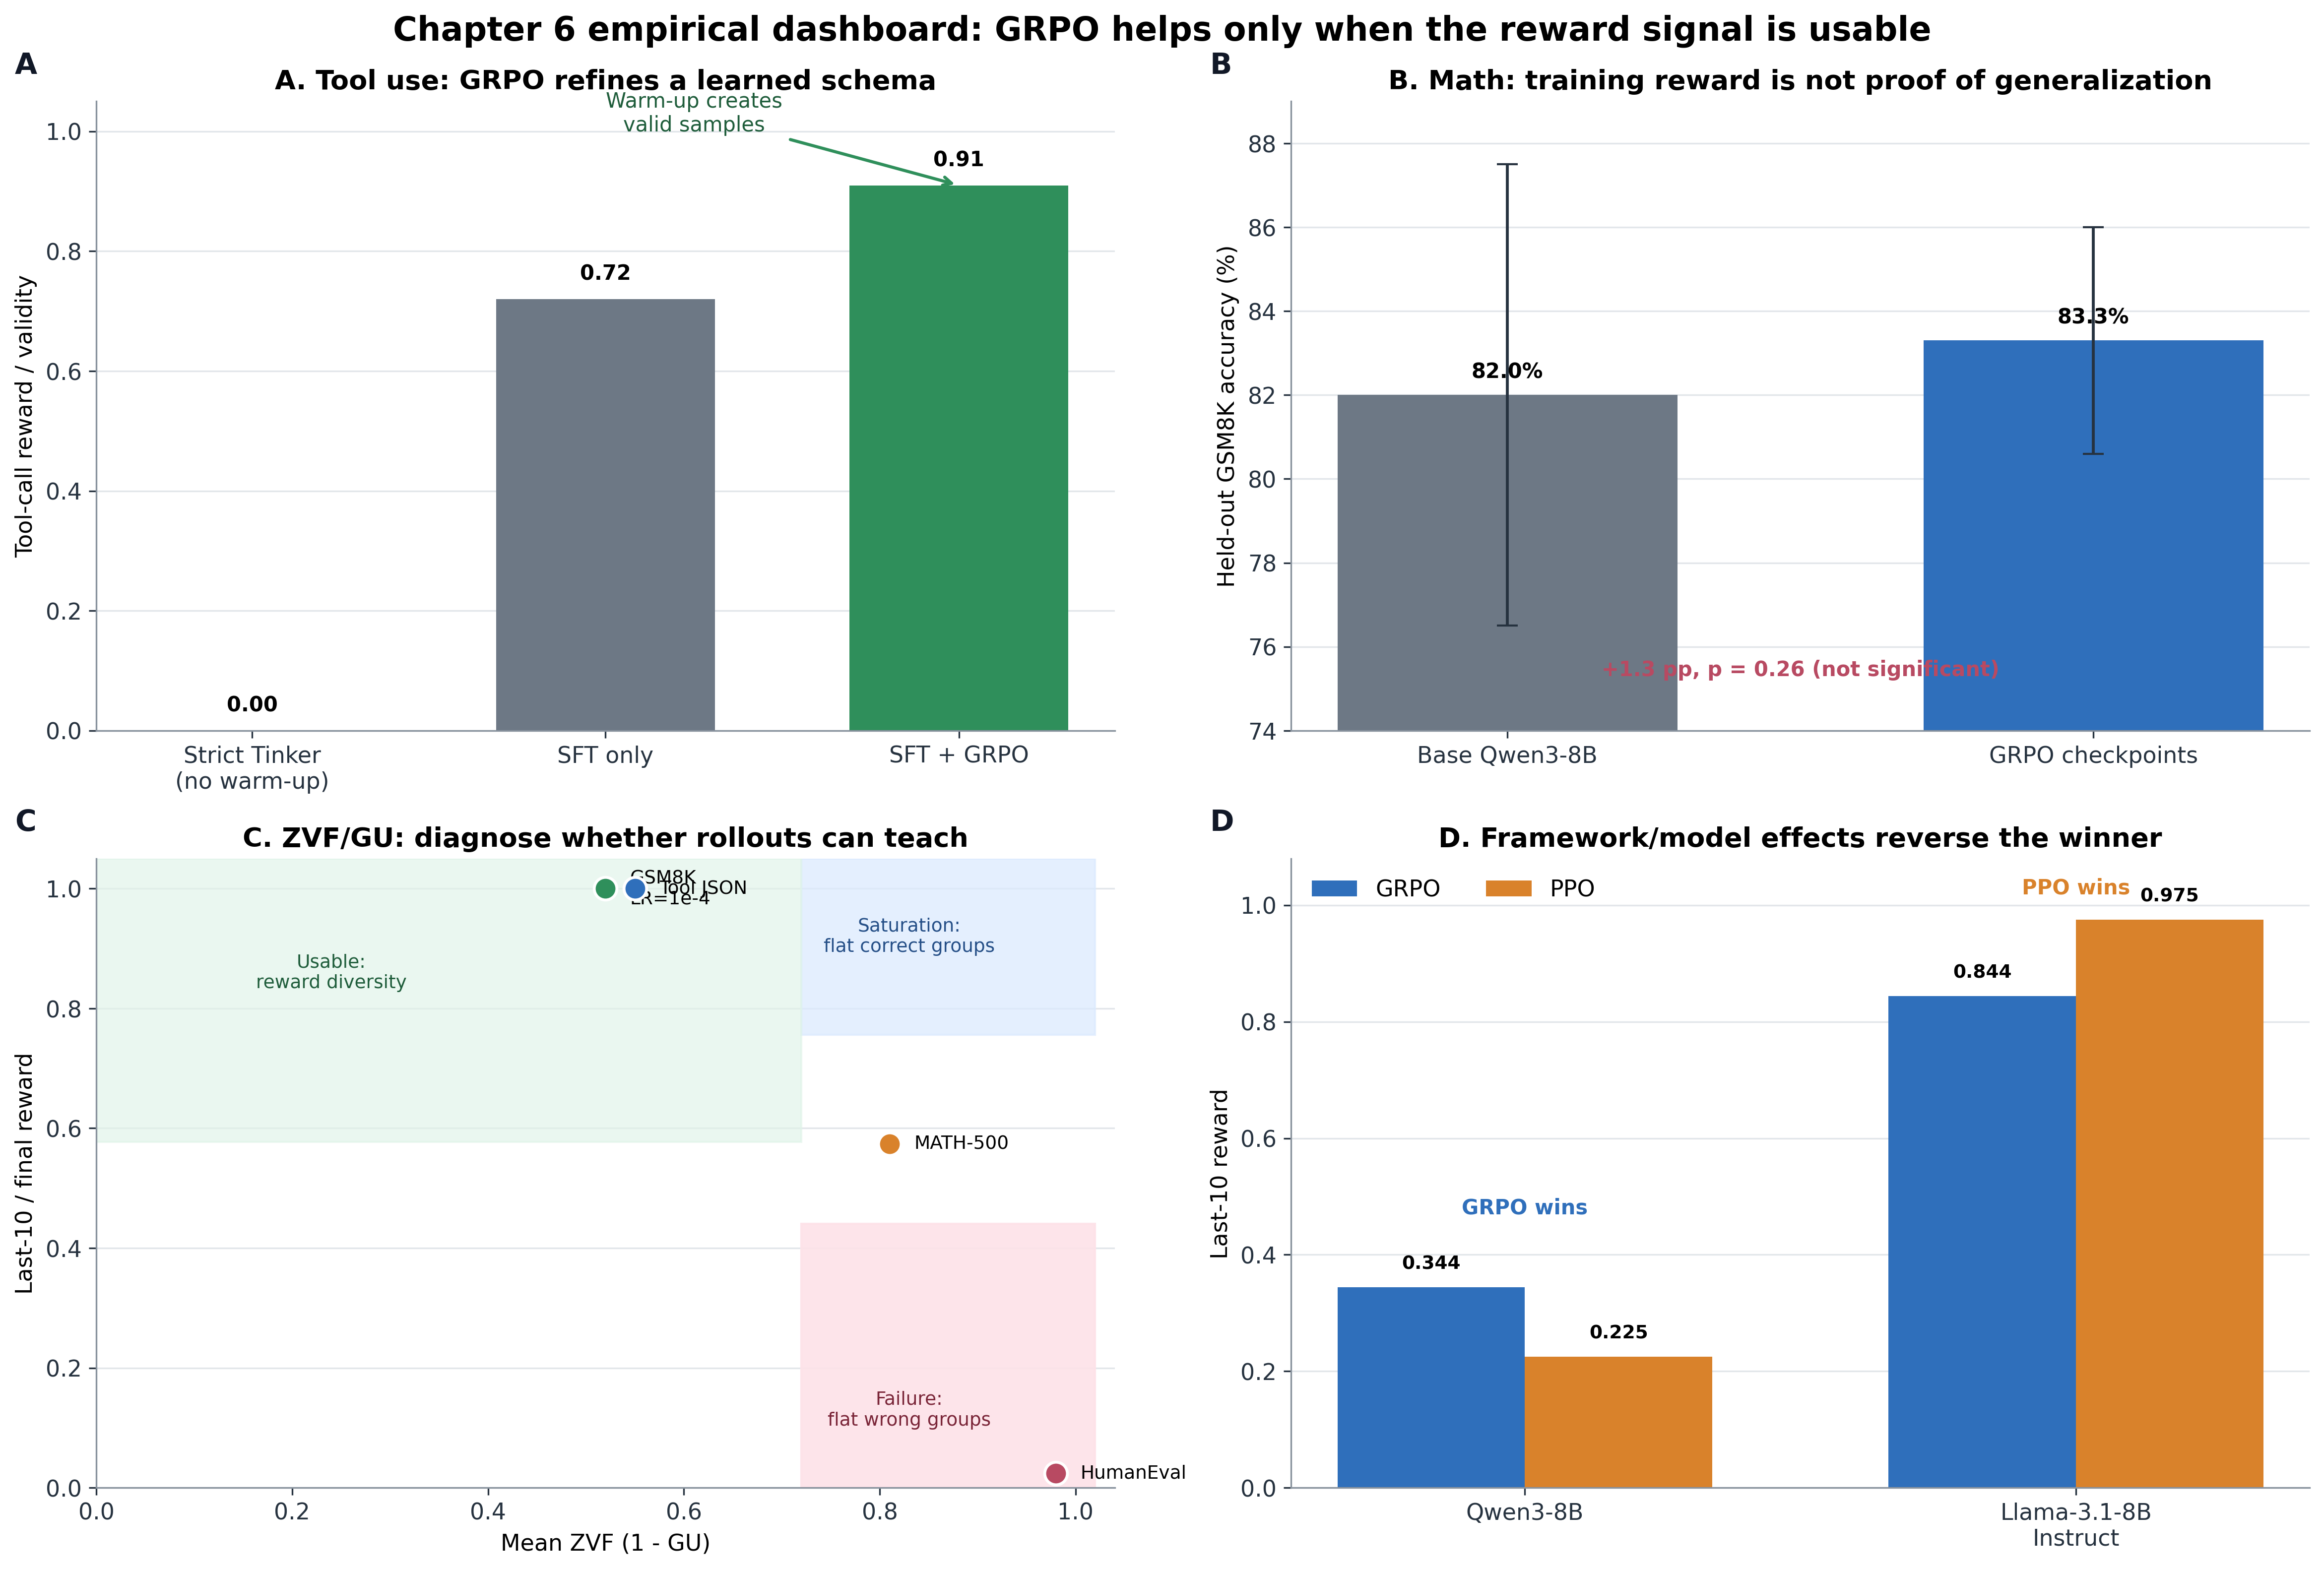
\includegraphics[width=\textwidth]{results_dashboard.pdf}
  \caption{Chapter 6 results dashboard. Panel A shows that GRPO improves tool-call format only after an SFT warm-up creates valid samples. Panel B shows that Qwen3-8B held-out GSM8K accuracy improves only from 82.0\% to 83.3\% after GRPO, which is not statistically significant ($p=0.26$). Panel C shows how ZVF separates usable reward diversity from flat wrong groups and flat saturated groups. Panel D shows that the recorded Qwen3-8B comparison favors GRPO, while the recorded Llama-3.1-8B-Instruct comparison favors PPO.}
  \label{fig:results-dashboard}
\end{figure}

Table~\ref{tab:rq-verdicts} connects each research question to its strongest supporting evidence and to the counter-evidence that limits the claim. The table is deliberately more cautious than a leaderboard because the experimental campaign combines controlled internal ablations, external team-member runs, partial frontier runs, and backend comparisons. Pooling all of them into one ranking would make the thesis simpler but less true. The appropriate synthesis is conditional: if the model already samples mixed-quality completions, GRPO can amplify that prior; if all sampled completions receive the same reward, GRPO has little useful gradient information; if the framework changes, the algorithmic conclusion may change as well.

\begin{table}[ht]
\centering
\caption{Research-question verdicts and supporting evidence.}
\label{tab:rq-verdicts}
\small
\begin{tabularx}{\textwidth}{p{2.45cm}p{4.05cm}p{4.05cm}X}
\toprule
Research question & Strongest evidence & Counter-evidence or limitation & Verdict\\
\midrule
Structured tool-call emission & Sandhya's SFT-warmed tool-calling pipeline improves from 0.72 under SFT to 0.91 after GRPO on the 3B model. & Strict Tinker tool-use runs without warm-up remain at 0\% reward, so schema-heavy tasks are too sparse when the model cannot already sample valid calls. & GRPO refines structured tool-call behavior after warm-up; it does not establish full interactive tool use without execution-level evaluation.\\
Math scaling and instruction tuning & GSM8K training trajectories improve for several instruction-tuned Qwen and Llama runs; Llama-3.1-8B-Instruct produces usable reward while base variants remain near zero. & Held-out Qwen3-8B evaluation improves only from 82.0\% to 83.3\% ($+1.3$ pp, $p=0.26$), so training reward does not establish generalization. & Instruction-tuned priors dominate small-model GRPO; held-out math improvement is not proven by the available evidence.\\
GRPO versus PPO & On Qwen3-8B, GRPO has a stronger recorded last-10 reward than PPO (0.344 versus 0.225). & On Llama-3.1-8B-Instruct, PPO beats the corresponding GRPO run (0.975 versus 0.844 last-10 reward). & Algorithm labels are insufficient; model family and backend implementation are first-class experimental variables.\\
Failure diagnostics & The 10x campaign shows high ZVF both when weak models produce indistinguishable wrong groups and when easy tasks saturate. & ZVF is a trajectory diagnostic, not a final capability benchmark; it must be interpreted with reward level and task difficulty. & ZVF/GU are the project's most reusable practical contribution because they identify wasted rollout compute early.\\
Mixed-group sampling condition & The task hierarchy places tool-use JSON and GSM8K above MATH-500 and HumanEval under the central Tinker GRPO setup. & Madhu's external HumanEval pipeline passed 141/164 problems by leveraging partial rewards and SFT warm-up. & The $1/G$ rule is only a sampling heuristic; the more precise condition is whether groups avoid the all-wrong and all-correct regimes.\\
\bottomrule
\end{tabularx}
\end{table}

\section{Base-Policy Hit Rate and Reward Diversity Indicate Whether GRPO Has a Learning Signal}
\label{sec:keystone-hit-rate}

This section is the empirical centre of the chapter. It states the project's sharpest diagnostic claim, tests it against recorded runs, and reframes every other result in Chapter~\ref{ch:results} in terms of measurable sampling conditions rather than a vague notion of task difficulty.

\subsection*{From $1/G$ intuition to mixed-group probability}

The intuitive threshold referenced elsewhere in this report---that GRPO needs base-policy zero-shot success rate $p_0>1/G$ to avoid ZVF collapse---is an \emph{expected-one-success heuristic}. It marks the point at which the expected number of correct samples per group is approximately one. It is not a strict necessary condition: learning can occasionally occur below it, but becomes increasingly sample-inefficient as $p_0 G \to 0$. What the GRPO estimator actually requires is a \emph{mixed-reward group}, which is the quantity the recent zero-variance-prompt literature has begun to name post hoc~\citep{rlzvp2025,rcgrpo2026}. Under sparse binary reward, a group of size $G$ drawn i.i.d.\ from a policy with per-sample success probability $p_0$ is \emph{usable} (delivers nonzero standard deviation, nonzero advantage, and a non-vacuous update) iff the group is neither all wrong nor all correct. The probability of that event is
\begin{equation}
  P\!\left(\text{usable group}\right) \;=\; 1 \;-\; (1-p_0)^{G} \;-\; p_0^{G},
  \label{eq:usable-group}
\end{equation}
and the project-level diagnostic $\zvf$ is its empirical complement. Equation~\eqref{eq:usable-group} reduces to $p_0 G$ for small $p_0$ (recovering the $1/G$ intuition), peaks at $p_0=0.5$, and drops symmetrically as $p_0\to 1$ (the saturation regime). Increasing $G$ is only a partial rescue: the cold-start term $(1-p_0)^G$ decays geometrically with $G$, but the saturation term $p_0^G$ then starts to dominate once the policy improves. The operational framing is therefore stronger than ``sparse rewards are hard''---GRPO's finite-sample learning signal depends on the probability of observing mixed groups, which is a joint property of base policy, group size, and reward function.

\subsection*{Keystone empirical table}

Table~\ref{tab:hit-rate-keystone} connects the major task families in this report to measured or inferred base-policy hit rate, model-implied usable-group probability, observed initial ZVF, and final reward outcome. The hit rates are taken under the exact training-time reward parser and decoding configuration used during GRPO when available, not under a greedy held-out evaluator. Inferred values are flagged: they are recovered from the observed initial ZVF and reward floor rather than measured directly, because the training logs for those runs do not include a dedicated zero-shot probe.

\begin{table}[ht]
\centering
\caption{Base-policy hit rate $p_0$, model-implied usable-group probability $P(\text{usable})$ from Eq.\ ~\eqref{eq:usable-group}, observed initial ZVF, and final reward outcome for representative task families. Values are a first-order diagnostic check, not a calibrated predictor of final performance.}
\label{tab:hit-rate-keystone}
\small
\setlength{\tabcolsep}{3pt}
\begin{tabularx}{\textwidth}{@{}p{0.21\textwidth}cccccX@{}}
\toprule
Task / setting & $p_0$ & $G$ & $P(\text{usable})$ & Initial ZVF & Last-10 & Interpretation\\
\midrule
GSM8K held-out base control\textsuperscript{\dag} & 0.820 & 32 & $\approx1.00$ & 0.00 & 0.833 & High aggregate hit rate supports mixed groups, but the held-out GRPO lift is non-significant.\\
SFT-warmed tool-call pipeline\textsuperscript{\ddag} & 0.720 & 32 & $\approx1.00$ & 0.20 & 0.910 & Warm-up moves the policy into a region where GRPO can refine format compliance.\\
Strict tool-use without warm-up\textsuperscript{*} & $\approx0$ & 32 & $\approx0$ & 1.00 & 0.000 & Schema-only reward is too sparse before the model can sample valid calls.\\
Central binary HumanEval\textsuperscript{*} & $\ll1/G$ & 32 & $\approx0$ & 1.00 & 0.024 & Functional pass/fail reward produced no useful signal in this setup.\\
\bottomrule
\end{tabularx}
\vspace{0.35em}
\begin{minipage}{0.96\textwidth}
\footnotesize
\textsuperscript{*}Inferred from initial ZVF and reward floor; explicit probe runs are scheduled in Future Work (§\ref{sec:future-work}). \textsuperscript{\dag}Predicted $P(\text{usable})$ uses the aggregate $p_0=0.820$ from the held-out base-model control. \textsuperscript{\ddag}Aggregate $P(\text{usable})$ is near 1, but per-prompt $p_0$ is bimodal, which is why the observed ZVF is 0.20 rather than $\approx 0$.
\end{minipage}
\end{table}

\subsection*{Group-size cross-check on Qwen3-8B GSM8K}

Equation~\eqref{eq:usable-group} is also consistent with the group-size trajectory recorded in the structural-ceiling campaign. For Qwen3-8B on GSM8K under a binary reward, the last-10 reward progression measured in the project's markdown artefact was $23.8\%$ at $G{=}4$, $24.4\%$ at $G{=}8$, $36.2\%$ at $G{=}16$, and $54.7\%$ at $G{=}32$. That order is consistent with the sampling model: at very small $G$, $(1-p_0)^G$ is the binding term and the group often collapses to all-wrong even though the aggregate $p_0$ is nontrivial; raising $G$ reduces that term geometrically and can unlock the gradient. Past $G{=}32$ the marginal return can turn over because $p_0^G$ begins to dominate once the task saturates. This reframes the inverted-U in group size reported in the paper companion as one possible mechanistic explanation, not as a proof that group size alone controls learning.

\subsection*{Reframing of the task hierarchy}

The stark contrast between successful structured tasks (Tool-Use, GSM8K) and failed semantic tasks (HumanEval, MATH-500) under the central Tinker GRPO setup is the most visible symptom of the mechanism formalized in §\ref{sec:keystone-hit-rate}. Because GRPO does not use a learned value function to estimate partial progress, it relies entirely on the base policy $\pi_\theta$ spontaneously generating at least one correct answer within a sampled group of size $G$---or, more precisely, on $P(\text{usable group})$ in Eq.\ ~\eqref{eq:usable-group} being comfortably above the ZVF$=1.00$ deadlock that paralyses binary-reward GRPO.

Tool-Use and GSM8K succeed in the recorded setup not because they are structural in the abstract, but because the model and reward combination can already produce mixed-quality samples. This yields low initial ZVF and provides the differential reward signal required to bootstrap optimization. Conversely, HumanEval and MATH-500 do not learn reliably in the central Tinker ablation because the probability of sampling a perfectly executing Python script or a fully accepted math solution is very low under the sparse verifier. In many sampled groups, every sample is wrong, the standard deviation $\sigma_r$ collapses to $\epsilon$, and the gradient carries little useful ordering information.

This mechanism helps resolve the apparent contradiction of external team runs. Madhu's external Qwen3-8B pipeline solved 141 of 164 HumanEval problems (86\% pass rate), while the central structural-ceiling HumanEval run yielded a total null. The external success does not show that the central binary-reward setup was sufficient; it shows that code generation is not intrinsically impossible for GRPO when the setup changes. Dense partial-credit reward (AST validity, staged assert passing) and supervised warm-up give the model intermediate breadcrumbs, lifting the chance of mixed groups above the ZVF$=1.00$ deadlock that paralyses binary-reward GRPO.

\paragraph{Relation to prior work.}
The original DeepSeek-Math and DeepSeek-R1 descriptions of GRPO~\citep{shao2024deepseekmath,deepseek2025r1} formalise the group-relative advantage but do not foreground the sampling-floor condition below which the estimator receives no useful ordering signal. Equation~\eqref{eq:usable-group} is a simple diagnostic model for that condition: it converts the empirical observation that GRPO ``fails on hard tasks'' into a testable statement about base-policy sampling, group size, and reward design, and it motivates two rescue directions (large-$G$ sampling and dense partial rewards) that are consistent with exploration-bottleneck arguments in sparse-reward RL.

\section{Boundary Cases and the External Dense-Reward Rescue}
\label{sec:structure-semantics}

\begin{figure}[ht]
  \centering
  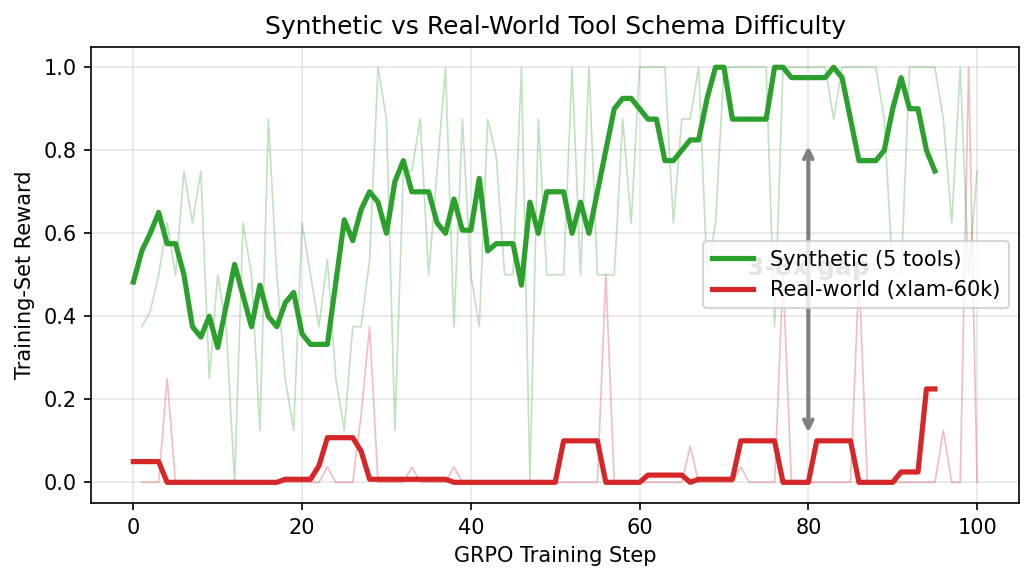
\includegraphics[width=\textwidth]{fig3_synthetic_vs_real.png}
  \caption{Comparison of synthetic versus real data environments, illustrating that GRPO is highly sensitive to base-policy hit rate and reward density rather than to semantics in the abstract.}
  \label{fig:synthetic-vs-real}
\end{figure}

The stark contrast between successful structured tasks (Tool-Use, GSM8K) and failed semantic tasks (HumanEval, MATH-500) under the central Tinker GRPO setup is the most visible symptom of the mechanism formalized in §\ref{sec:keystone-hit-rate}. Because GRPO does not use a learned value function to estimate partial progress, it relies entirely on the base policy $\pi_\theta$ spontaneously generating at least one correct answer within a sampled group of size $G$---or, more precisely, on $P(\text{usable group})$ in Eq.\ ~\eqref{eq:usable-group} being comfortably above the ZVF$=1.00$ deadlock that paralyses binary-reward GRPO.

Tool-Use and GSM8K succeed in the recorded setup not because they are structural in the abstract, but because the model and reward combination can already produce mixed-quality samples. This yields low initial ZVF and provides the differential reward signal required to bootstrap optimization. Conversely, HumanEval and MATH-500 do not learn reliably in the central Tinker ablation because the probability of sampling a perfectly executing Python script or a fully accepted math solution is very low under the sparse verifier. In many sampled groups, every sample is wrong, the standard deviation $\sigma_r$ collapses to $\epsilon$, and the gradient carries little useful ordering information.

This mechanism helps resolve the apparent contradiction of external team runs. Madhu's external Qwen3-8B pipeline solved 141 of 164 HumanEval problems (86\% pass rate), while the central structural-ceiling HumanEval run yielded a total null. The external success does not show that the central binary-reward setup was sufficient; it shows that code generation is not intrinsically impossible for GRPO when the setup changes. Dense partial-credit reward (AST validity, staged assert passing) and supervised warm-up give the model intermediate breadcrumbs, lifting the chance of mixed groups above the ZVF$=1.00$ deadlock that paralyses binary-reward GRPO.

\paragraph{Relation to prior work.}
The original DeepSeek-Math and DeepSeek-R1 descriptions of GRPO~\citep{shao2024deepseekmath,deepseek2025r1} formalise the group-relative advantage but do not foreground the sampling-floor condition below which the estimator receives no useful ordering signal. Equation~\eqref{eq:usable-group} is a simple diagnostic model for that condition: it converts the empirical observation that GRPO ``fails on hard tasks'' into a testable statement about base-policy sampling, group size, and reward design, and it motivates two rescue directions (large-$G$ sampling and dense partial rewards) that are consistent with exploration-bottleneck arguments in sparse-reward RL.

\section{Instruction Tuning Dominates Small-Model GRPO}
\label{sec:instruction-tuning}

\begin{figure}[ht]
  \centering
  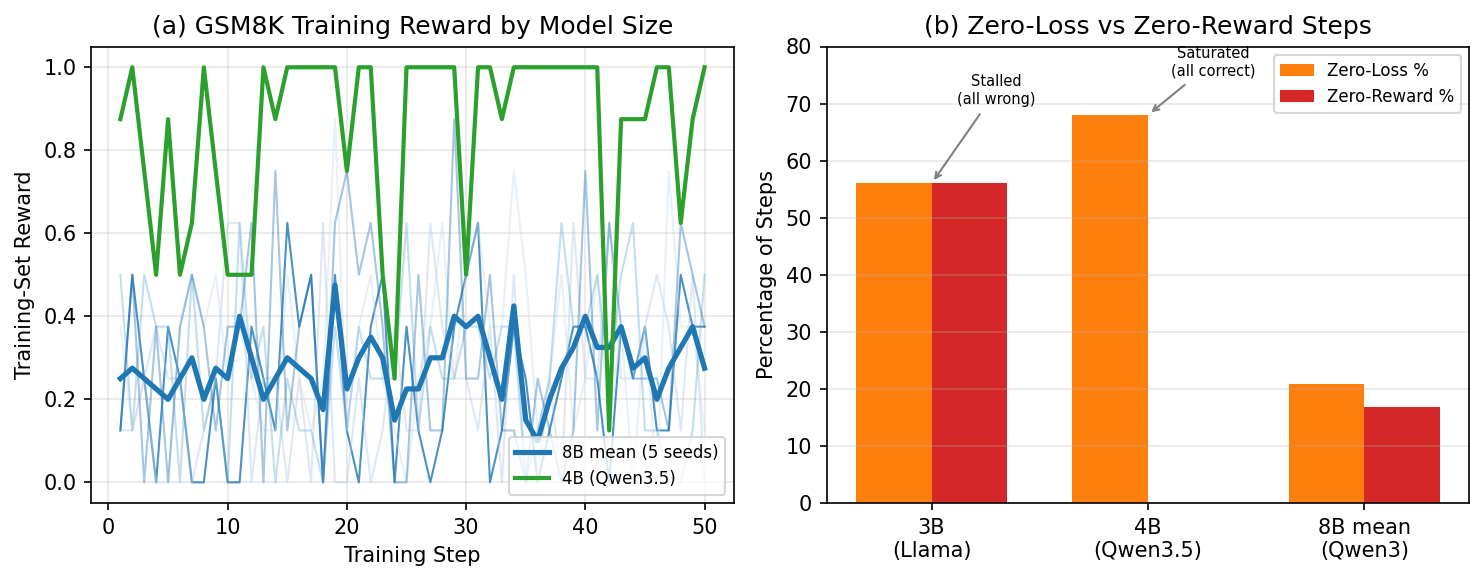
\includegraphics[width=\textwidth]{fig1_capacity_threshold.png}
  \caption{Capacity threshold demonstrating how model scale and instruction tuning interact with GRPO gradient availability. Models below the capability threshold suffer immediate ZVF saturation.}
  \label{fig:capacity-threshold}
\end{figure}


The model-size ladder and base-to-instruct comparisons show that GRPO does not reliably bootstrap a weak base model into a capable reasoner under this sparse-reward setup. Below roughly the 8B-instruct regime in the recorded experiments, reward variance frequently collapses immediately. The Llama base-to-instruct contrast is especially large: the instruction-tuned model produces usable GSM8K reward while the base model remains near zero. The held-out Qwen3-8B result in Figure~\ref{fig:results-dashboard}B sharpens this conclusion rather than weakening it: even when training reward improves, final GSM8K test accuracy rises only 1.3 percentage points over the base control and is not statistically significant. The practical conclusion is therefore conservative: SFT or instruction tuning is an enabling control in this corpus, and GRPO is a refinement stage whose gains must be checked outside the rollout distribution.

\section{ZVF Flags Failure and Wasted Compute}
\label{sec:zvf-results}

\begin{figure}[ht]
  \centering
  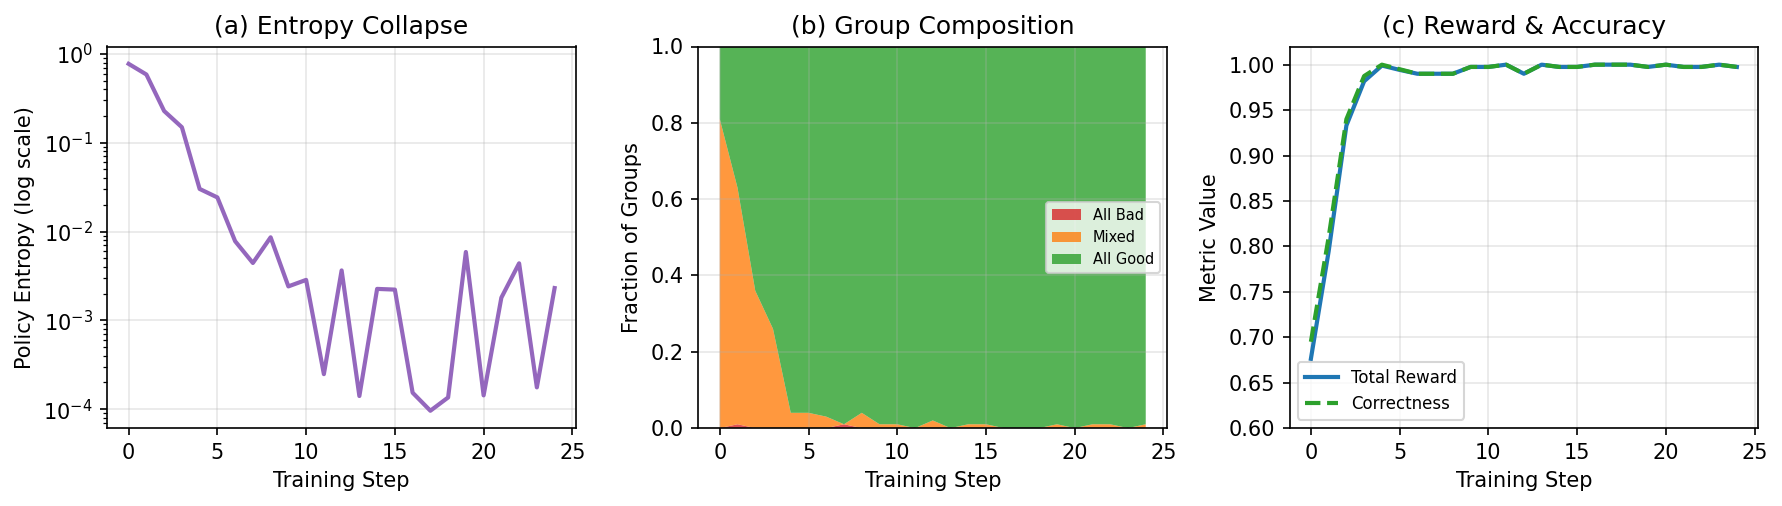
\includegraphics[width=\textwidth]{fig2_diagnostics.png}
  \caption{Reward and diagnostic trajectories across key ablation runs. ZVF and GU provide an early indicator of whether a run has useful learning signal or is merely wasting compute.}
  \label{fig:diagnostics-curves}
\end{figure}


ZVF explains several otherwise confusing results. A run can fail because all outputs are wrong, or it can saturate because all outputs are correct. Both states produce flat reward groups, but they have opposite meanings. Figure~\ref{fig:results-dashboard}C makes this diagnostic distinction visible: low reward with high ZVF is a zero-gradient failure mode, while high reward with high ZVF is saturation rather than continued learning. For weak models and hard tasks, high ZVF at step zero indicates that the task is beyond the current policy's sampling distribution. For easy format tasks, rising ZVF later in training indicates mastery followed by wasted updates. ZVF must therefore always be interpreted jointly with reward level---the same flat-group signature means opposite things depending on where the reward curve sits. GU is ZVF's complement and a compute-efficiency measure: a run with high reward but low GU may already be done, while a run with low reward and low GU needs curriculum, easier prompts, larger group size, or SFT warm-up.

To test whether this triage rule has prospective value, I ran a pseudo-prospective validation over the completed step logs with recorded reward, ZVF, and GU. The validation froze the rule to the first five logged optimization steps and computed outcomes only from the final ten logged steps. Across 52 raw candidate records, de-duplication by run identity produced 22 independent usable runs. A fixed early-failure rule---mean early ZVF $\ge 0.80$ and mean early reward $\le 0.05$---identified both collapsed runs with zero false positives (TP=2, FP=0, TN=20, FN=0). This supports ZVF as an early collapse diagnostic, but the positive failure count is only two. It does not prove that ZVF continuously ranks final performance among non-collapsed runs: early ZVF versus late reward had Spearman $\rho=-0.16$ with a bootstrap 95\% interval of $[-0.63,0.43]$, and adding early ZVF to early reward changed leave-one-run-out $R^2$ only from $0.885$ to $0.888$. \textbf{The defensible conclusion is therefore that ZVF is a collapse/saturation triage diagnostic, not a calibrated performance predictor.} In the available logs, early high-ZVF/low-reward states marked the two collapsed runs, while non-collapsed run quality still depended on task, model, and backend.

\paragraph{Relation to prior work.}
Recent GRPO theory characterises the group-relative policy gradient as a $U$-statistic with known finite-sample and group-size properties~\citep{zhou2026demystify}, but that line of work is not primarily an experimenter-facing run-management protocol. Our contribution is complementary: the triage rule above translates the same variance behaviour into a concrete stop/redesign decision. The zero-variance-prompt literature~\citep{rlzvp2025} argues that zero-variance prompts can still be useful if handled specially (e.g.\ with modified advantage estimators). Under \emph{standard} GRPO, our finding is the operational counterpart: early high-ZVF/low-reward is a signal to change the experimental design---reshape the reward, add SFT, increase group size, or reduce task difficulty---before wasting rollout compute.

\section{Group Size and Learning Rate Trade Off Signal Against Cost}
\label{sec:g-lr}

The group-size ablation shows that many group sizes can converge on easy-enough tasks, but they differ in how long they preserve gradient signal. In the structural-ceiling campaign, $G=32$ had the best balance of mean GU and delayed saturation, while $G=64$ had diminishing returns for twice the rollout cost. The learning-rate ablation shows a similar tradeoff. Low learning rates preserve signal longer but converge more slowly. High learning rates can reach high reward quickly but saturate early or produce transient instability. The full-data correction for LR=$3\times 10^{-4}$ is important: what looked like divergence in partial data later recovered, demonstrating why final reports should distinguish partial trajectories from completed runs.

\section{Framework Effects Are First-Class Results}
\label{sec:framework-effects}

The project initially treated frameworks as implementation details. The final evidence shows they are experimental variables. Tinker, TRL, Modal PPO, and classical PPO baselines expose different sampling loops, optimizer choices, rollout handling, logging, and infrastructure constraints. The PPO comparison in Figure~\ref{fig:results-dashboard}D is the strongest warning against overclaiming: GRPO is better in the recorded Qwen3-8B comparison, while PPO is better in the recorded Llama-3.1-8B-Instruct comparison. \textbf{The reversal, not the individual direction, is the finding.} Because the evidence is not a fully crossed factorial design, the claim is deliberately \emph{methodological rather than causal}: we do not claim that framework \emph{caused} the reversal. We claim that the reversal shows model family and backend must be controlled before algorithm-level conclusions are published. The safer interpretation is that GRPO-style post-training is sensitive to the complete training stack, and that PPO/GRPO/DPO labels are not complete specifications of an experimental condition.

\paragraph{Relation to prior work.}
The direction-flip observed here directly challenges the prevailing algorithm-comparison style in RLHF/RLVR, where PPO~\citep{schulman2017proximal}, DPO~\citep{rafailov2024direct}, and GRPO~\citep{shao2024deepseekmath} are described as self-contained methods and benchmarked pairwise on a single model family with a single library. It revives, for LLM post-training, the reproducibility critique that Henderson et al.~\citep{henderson2018deep} raised for classical deep RL: nominal algorithm identity is not sufficient to specify an experimental condition.

\section{Failure Taxonomy and Diagnostic Action Map}
\label{sec:failure-taxonomy}

The most useful form of the results is not a single leaderboard, but a diagnostic map from symptoms to interventions. The project repeatedly shows that the same surface metric can mean different things depending on reward level, task difficulty, and timing. High ZVF, for example, can indicate either total failure or solved-task saturation. Training reward can rise while held-out accuracy barely moves. A framework comparison can reverse when the model family changes. Table~\ref{tab:failure-taxonomy} therefore converts the main empirical findings into an action map for future GRPO and PPO runs.

\begin{table}[ht]
\centering
\caption{Failure taxonomy and diagnostic action map for RL fine-tuning runs.}
\label{tab:failure-taxonomy}
\small
\begin{tabularx}{\textwidth}{p{3.15cm}p{3.35cm}p{3.7cm}X}
\toprule
Observed symptom & Likely mechanism & Evidence in this project & Recommended next action\\
\midrule
Low reward and high early ZVF & The base model samples no correct completions inside the group, so GRPO has no differential reward signal. & HumanEval, MATH-style, and strict tool-use failures under sparse binary rewards. & Measure zero-shot hit rate first; add SFT warm-up, partial rewards, curriculum, or larger $G$ before spending more RL compute.\\
Low reward but nonzero reward variance & The task is reachable, but the policy is still weak or the reward is noisy. & Some GSM8K and sensitivity runs preserve GU before reward stabilizes. & Continue briefly, then check whether reward gains survive held-out evaluation.\\
High reward and rising ZVF & The run may have saturated rather than failed. & Easy arithmetic and format-heavy settings can become flat because most samples receive the same high reward. & Stop or reduce update frequency; spend compute on harder prompts or held-out checks.\\
Training reward improves but held-out accuracy is flat & The policy may be exploiting the rollout distribution, parser, or prompt slice. & Qwen3-8B held-out GSM8K improves only from 82.0\% to 83.3\%, not statistically significant. & Treat training reward as a dynamics metric, not a capability claim; require held-out, adversarial, or task-family transfer evaluation.\\
Recorded PPO/GRPO direction flips across settings & Algorithm, model family, backend, and reward implementation are entangled. & Qwen3-8B favors GRPO in the recorded comparison, while Llama-3.1-8B-Instruct favors PPO. & Report backend and model-family controls alongside algorithm labels.\\
Tool-call format improves but semantic success is uncertain & The reward may overemphasize schema validity relative to downstream task correctness. & SFT-warmed tool-use results improve strongly, while strict Tinker tool-use remains brittle. & Split rewards and evaluation into syntax, tool selection, argument correctness, execution success, task completion, and generalization.\\
\bottomrule
\end{tabularx}
\end{table}

This taxonomy is also a safeguard against over-interpreting negative results. A failed run can mean that GRPO is inappropriate for the task, but it can also mean that the reward is too sparse, the group size is too small for the base hit rate, the prompt distribution is too hard for cold start, or the framework is not matched to the comparison. Conversely, a successful run can mean genuine generalization, but it can also mean that the rollout environment has become easy to exploit. The diagnostic contribution of ZVF and GU is that they make these distinctions visible early enough to change the experiment while compute is still being spent.

\chapter{Discussion}
\label{ch:discussion}

The Results chapter gives the empirical verdicts. This chapter interprets those verdicts as a set of design rules for future post-training studies. The central point is that GRPO should not be treated as a generic reasoning-improvement switch. In this project, its useful regime is narrower and more operational: it refines behaviors that are already inside the base model's sampling distribution and already produce within-group reward diversity. When those conditions are absent, the training loop can run successfully while producing little useful optimization.

\section{Separating Capability Claims from Dynamics Claims}
\label{sec:capability-vs-dynamics}

The dissertation-style evidence hierarchy in this report separates three kinds of claims. Implementation claims are supported by successful backend execution, checkpoint capture, and reproducible scripts. Dynamics claims are supported by reward, ZVF, GU, and trajectory logs. Capability claims require held-out or otherwise distribution-shifted evaluation. This distinction explains why the Tinker live run is important but modest: it proves that hosted execution and artifact capture worked, not that the trained policy is better than a base model. It also explains why training reward curves remain valuable even when held-out accuracy is not significant: they reveal when reward variance exists, when it collapses, and when framework effects dominate.

The strongest empirical conclusion is therefore diagnostic rather than leaderboard-based. ZVF and GU do not replace accuracy, pass rate, or human preference evaluation. They explain whether a run has a usable learning signal before those downstream metrics are interpreted. A low-reward high-ZVF run is not merely low performing; it is structurally unable to provide group-relative credit assignment under the current reward. A high-reward high-ZVF run is not necessarily failing; it may be saturated. Treating both as the same flat trajectory would hide the practical decision the experimenter needs to make.

\section{Design Rules for Future Critic-Free RL Studies}
\label{sec:design-rules}

Table~\ref{tab:design-rules} converts the project findings into design rules. These rules are intentionally operational because most failed RL fine-tuning runs do not fail at the level of abstract algorithm choice; they fail because the reward is too sparse, the base policy cannot sample any correct completions, the group size is mismatched to hit rate, or the framework is not matched to the comparison.

\begin{table}[ht]
\centering
\caption{Design rules implied by the project evidence.}
\label{tab:design-rules}
\small
\begin{tabularx}{\textwidth}{p{3.25cm}p{4.25cm}X}
\toprule
Rule & Why it follows from the evidence & What to do in future work\\
\midrule
Measure base hit rate before GRPO & If the base model rarely samples any rewarded completion under the intended reward parser and decoding setup, sampled groups are likely to be uniformly wrong and ZVF will collapse. & Run a zero-shot or few-shot preflight and estimate $1-(1-p_0)^G-p_0^G$ before launching RL.\\
Use partial rewards for hard semantic tasks & Binary rewards on HumanEval-style or MATH-style tasks can produce no within-group ordering even when some completions are partially useful. & Reward syntax, intermediate tests, decomposition steps, or verifier progress separately from final success.\\
Treat framework as an experimental factor & PPO and GRPO comparisons changed direction across model families and backends in the recorded runs. & Report library, sampler, optimizer, rollout, and checkpoint details as part of the method, not as incidental plumbing.\\
Separate training dynamics from capability & Reward can improve while held-out accuracy barely changes, especially under narrow rollout distributions. & Require held-out, adversarial, or task-family transfer evaluation before claiming capability improvement.\\
Stop or redirect saturated runs & High reward with high ZVF can mean the task is solved and further updates waste rollout compute. & Move to harder prompts, reduce updates, or shift compute to held-out evaluation.\\
\bottomrule
\end{tabularx}
\end{table}

\section{Implications for Structured-Output and Agentic Evaluation}
\label{sec:agentic-implications}

Structured-output and agentic fine-tuning are especially sensitive to this evidence hierarchy because the surface behavior can be misleading. A model can emit valid JSON while choosing the wrong tool. It can pass a format checker while failing the user task. It can improve on a narrow math reward while not improving held-out reasoning. The practical implication is that future tool-oriented RL pipelines should decompose evaluation into syntax, tool selection, argument correctness, execution success, task completion, and generalization. GRPO may be appropriate for the early structured-output stages after SFT warm-up, but full agentic claims require stronger verifiers and broader evaluation.

The project also suggests a useful order of operations. First, establish whether the base model can sample any valid or partially valid behavior under the intended reward. Second, use SFT or instruction tuning to raise the mixed-group probability if the task is schema-heavy or reward-sparse. Third, run GRPO only after reward diversity is visible. Fourth, monitor ZVF and GU during the run to decide whether to continue, stop, or redesign the reward. Fifth, evaluate the final checkpoint outside the rollout distribution. This ordering is more conservative than a benchmark-first workflow, but it is better matched to the observed failure modes.

\section{What Should Not Be Claimed}
\label{sec:not-claimed}

The evidence does not justify the claim that GRPO broadly improves small-model reasoning. It also does not justify a universal ranking of GRPO over PPO, or of one training backend over another. The correct conclusion is conditional: critic-free RL is useful when the model already has a behavioral prior and the reward function produces within-group variance. In the absence of that contrast, compute can be spent without meaningful gradient information. This limitation is not a defect in the report; it is the main systems lesson produced by the experiment campaign.

\chapter{Limitations and Threats to Validity}
\label{ch:limitations}

The main conclusions are deliberately conditional because the evidence base is broad but uneven. The experiments are strong enough to identify recurring failure modes in critic-free RL fine-tuning, especially reward-variance collapse, but they are not large enough to establish universal scaling laws for all models, rewards, and infrastructures.

\section*{Internal Validity}
Some runs differ in more than one experimental factor. Model family, instruction tuning, backend implementation, decoding temperature, group size, reward parser, and checkpoint recovery all interact. This means that a raw reward difference cannot always be attributed to GRPO, PPO, model scale, or framework choice alone. The report mitigates this by separating completed ablations from external team-member runs and partial frontier runs, but residual confounding remains.

\section*{Construct Validity}
Several rewards measure proxies rather than the full target behavior. Tool-use experiments sometimes reward JSON validity, tool-name selection, or argument completion without proving end-to-end tool competence. Code-generation rewards depend on parser and test coverage, so a pass-rate number can miss hallucinated edge cases or brittle solutions. Mathematical rewards based on exact-match parsing can also undercount equivalent answers or overcount formatting shortcuts. ZVF and GU are therefore diagnostics of reward-signal structure, not direct measures of intelligence.

\section*{External Validity}
The results are most applicable to GRPO-style or PPO-style post-training of open-weight LLMs under verifiable or semi-verifiable rewards. They should transfer cautiously to other domains. Preference-only alignment, long-horizon interactive agents, multimodal policies, and proprietary frontier-model post-training may have different reward distributions and sampling behavior. The project also focuses heavily on GSM8K, MATH-like tasks, HumanEval-style code, and tool-call schemas; other domains may cross the cold-start threshold at different model sizes.

\section*{Statistical Conclusion Validity}
Held-out GSM8K evaluation provides stronger evidence than training trajectories, but the available held-out lift for Qwen3-8B is small and not statistically significant. Several ablations are single-run or low-seed because of compute limits. The pseudo-prospective ZVF validation is useful because it freezes early-step predictors and tests final-step outcomes, but it is still retrospective over existing logs and contains only two collapsed independent runs after de-duplication. The fixed ZVF rule should therefore be treated as a promising triage rule, not a calibrated production classifier.

\section*{Benchmark, Prompt, and Contamination Validity}
GSM8K, HumanEval, and MATH-style benchmarks are public, so strong base-model performance may partly reflect pretraining exposure rather than reasoning learned during this project. The held-out GSM8K control mitigates this by comparing the LoRA checkpoints against the same base model on the same 200 examples, but it does not eliminate contamination risk. Prompt templates and decoding settings are also plausible confounders: reward success can change when the answer format, chain-of-thought instruction, tool schema ordering, or sampling temperature changes. Future evaluations should include prompt perturbations, paraphrased or freshly generated math items, private unit tests, and tool schemas with reordered or paraphrased descriptions.

\section*{Reward and Optimization Pathologies}
Sparse binary rewards can confound three explanations: the model may lack the capability, the model may have the capability but fail to sample it under the chosen decoding regime, or the parser/verifier may fail to recognize partially correct or equivalent outputs. This is especially important for HumanEval and MATH-style tasks. The report's negative claim is therefore limited to the observed setup: under the available compute budget, parser, and reward design, learning was not observed. Modern GRPO critiques also warn that response length, group standard-deviation normalization, and clipping choices can bias optimization~\citep{liu2025r1zerocritical}. This artifact does not yet include systematic response-length tracking or reward-versus-length plots, so reward hacking and length bias remain important follow-up checks.

\section*{Artifact Hygiene and External Services}
The public submission archives intentionally exclude local credential files, API keys, W\&B state directories, private environment files, and cloud-service caches. The repository-level ignore rules include \texttt{.env}, \texttt{.env.*}, \texttt{.tinker\_api\_key}, \texttt{*.key}, \texttt{*.pem}, \texttt{*.token}, and \texttt{wandb/}. Local credentials detected during packaging were not inspected or printed in this report and should be rotated or revoked before any public release. Exact reproduction of hosted Tinker runs, W\&B dashboards, and private checkpoints may require external service permissions; the artifact therefore includes local summaries and scripts as the auditable source of truth.

\section*{Reproducibility Limits}
The report links each major claim to logs, scripts, figures, and summaries where possible, but not every external run has identical artifact completeness. Some checkpoints timed out, some frontier runs are partial, and team-member experiments used different repositories and evaluation conventions. The artifact bundle is sufficient to audit the reported conclusions, but a fully reproducible dissertation-grade replication would require a locked prompt set, frozen Docker images, fixed random seeds, uploaded checkpoints, and an automated evaluation harness for every experiment family.

\chapter{Conclusion and Future Work}
\label{ch:conclusion}

\section{Conclusion}
The project's final answer is nuanced. GRPO is useful when the model already has a behavioral prior and the reward function produces within-group variance. In that regime, it can reinforce structured outputs and improve some exact-answer tasks. GRPO is unreliable when the model is too weak under the chosen decoding setup or when the reward/parser is too sparse or brittle to differentiate completions. The key practical lesson is to monitor ZVF and GU early, treat instruction tuning and SFT warm-up as enabling controls, separate training reward from held-out generalization, and evaluate framework effects before making algorithmic claims.

The final report therefore reframes the capstone from ``GRPO improves small LLM reasoning'' to a sharper systems claim: critic-free RL can be effective for structured post-training, but its success depends on reward variance, base-model capability, instruction tuning, group size, task structure, and implementation framework. This is a more useful conclusion for practitioners because it explains both the positive tool-use results and the many null or unstable runs.

\section{Future Work}
\label{sec:future-work}
With the mixed-group sampling condition now formalized in §\ref{sec:keystone-hit-rate}, two falsification experiments would sharpen the mechanistic story. The zero-shot hit-rate mapping that earlier drafts treated as ``immediate next work'' is now the starting point of §\ref{sec:keystone-hit-rate}, so Future Work focuses on testing the boundaries of the sampling model rather than treating it as settled theory.

\begin{enumerate}
    \item \textbf{The Group-Size Rescue Experiment:} Eq.\ ~\eqref{eq:usable-group} suggests that for a hard task with $p_0\approx 1\%$, a standard group of $G=32$ will often fail ($P(\text{usable})\approx 0.27$, with effective ZVF higher in practice because of per-prompt variance), while $G=256$ should lift $P(\text{usable})$ above $0.9$ and escape the sampling floor. Running a difficult task---HumanEval binary reward on Qwen3-8B is the obvious candidate---with an aggressively large $G$ would test how much of the observed failure is inadequate sampling versus reward/parser brittleness or model capability.
    \item \textbf{The Partial Reward Rescue Experiment:} Implementing a dense, step-level reward for HumanEval (e.g., $+0.2$ for valid syntax, $+0.5$ for passing the first assert, $+1.0$ for all asserts) should push $p_0$ toward the middle of the distribution where $P(\text{usable})$ is maximal. If providing granular breadcrumbs reliably lowers ZVF and enables learning on the central Tinker pipeline, it would show that GRPO can learn in this domain once the exploration bottleneck is mitigated, and it would support the reward-density prediction of Eq.\ ~\eqref{eq:usable-group}.
\end{enumerate}

Additionally, a rigorous study ablating the degree of Supervised Fine-Tuning (SFT) useful before initiating GRPO could yield more efficient post-training pipelines---the SFT-warmed tool-use result in §\ref{sec:keystone-hit-rate} already hints that a $p_0$ of roughly $0.7$ is sufficient for $G=32$ GRPO to reach $0.9+$. Finally, scaling out the held-out evaluation suite to test the resilience of GRPO-trained models against reward hacking across wider domains remains an essential step for translating these methods into production environments.

\appendix
\chapter{Experiment Summary Tables}
\label{app:experiment-summary}

\begin{landscape}
\begingroup
\footnotesize
\setlength{\tabcolsep}{3pt}
\begin{longtable}{p{3.2cm}p{3.0cm}p{2.5cm}p{2.2cm}p{1.8cm}p{1.5cm}p{4.8cm}}
\caption{Condensed inventory of experiments considered in the final analysis.}\label{tab:condensed-inventory}\\
\toprule
Experiment block & Representative models & Method & Task & Status & Mean ZVF & Interpretation\\
\midrule
\endfirsthead
\toprule
Experiment block & Representative models & Method & Task & Status & Mean ZVF & Interpretation\\
\midrule
\endhead
Arithmetic RL & Llama-3.2-1B & GRPO & Arithmetic & Complete & --- & Validated the basic RL loop and reached perfect arithmetic accuracy.\\
Chat supervised learning & Llama / Qwen small models & SFT & Chat & Complete & --- & Verified supervised fine-tuning pipeline.\\
Preference shorter & Small instruct models & Preference optimization & Style control & Complete & --- & Demonstrated response-style shaping.\\
Off-policy distillation & Teacher to student setup & SFT and distillation & Reasoning transfer & Complete & --- & Established distillation as a strong non-RL baseline.\\
On-policy distillation & Teacher and student loop & KL minimization & Reasoning transfer & Complete & --- & Tested online distillation mechanics.\\
GSM8K cookbook & Small LLMs & GRPO & Math & Complete & --- & Bridged toy arithmetic and word-problem reasoning.\\
Sandhya tool calling & Qwen2.5 0.5B, 1.5B, 3B & SFT+GRPO & Tool use & Complete & 0.20 & Strong format and tool-call gains after warm-up.\\
Madhu code generation & Qwen3-8B & GRPO & HumanEval & Complete external & --- & Best code result, but protocol differs from central Tinker harness.\\
Mohammad math & Qwen3-4B & GRPO & Math & Complete external & --- & Small gain; illustrates that GRPO can be marginal.\\
Arumugam keywords & 0.5B model & DPO & Keyword generation & Complete external & --- & Positive low-data result; not a broad RL claim.\\
Tinker GSM8K scaling & Qwen, Llama, DeepSeek, Nemotron, Kimi & GRPO & GSM8K & Mixed & 0.60 & Revealed model-family and scale dependence.\\
Tinker tool-use cross-task & Qwen3-32B, Llama-8B-Instruct & GRPO & Tool use & Failed/\allowbreak zero & 1.00 & Strict tool-use without warm-up produced no reward signal.\\
10x benchmark hierarchy & Qwen3-8B & GRPO & Tool, GSM8K, MATH, HumanEval & Complete & 0.71 & Structure is easier than semantic code and hard math.\\
10x model-size ladder & Qwen 0.6B/1.7B/8B, Llama 1B/3B/8B & GRPO & GSM8K & Complete & 0.95 & Below 8B-instruct, ZVF dominates and learning fails.\\
10x group ablation & Qwen3-8B & GRPO & GSM8K & Complete & 0.52 & $G=32$ balances utilization and cost.\\
10x LR ablation & Qwen3-8B & GRPO & GSM8K & Complete & 0.45 & LR controls speed-saturation behavior; partial runs can mislead.\\
Constrained decoding & Qwen3-8B & GRPO & Tool use & Complete & --- & Decoder constraint was not the main confound.\\
Modal PPO & Qwen3-8B, Llama-8B-Instruct & PPO & GSM8K & Complete & --- & PPO can beat GRPO on Llama while trailing on Qwen.\\
Modal KL tracking & Qwen3-8B & PPO+KL & GSM8K & Failed & --- & Gradient error; useful implementation failure.\\
Modal HumanEval eval & Qwen3-8B & Evaluation & Code & Partial & --- & Timed out; partial pass rate only.\\
Held-out math evals & Qwen3.5-27B, Qwen3-32B & Evaluation & GSM8K held-out & Partial & --- & Timeout-limited; held-out math only.\\
TRL GRPO baseline & Qwen2.5-0.5B & TRL-GRPO & Math & Complete & --- & Multi-seed mean around 0.734 in the recorded summary.\\
Classical PPO baselines & SB3, CleanRL, Tianshou & PPO & Math & Complete & --- & Near-zero performance; LLM backbone is necessary.\\
Wave sensitivity & Qwen3-8B & GRPO & GSM8K & Complete & 0.40 & Hyperparameters tune an existing signal; they do not manufacture one.\\
Bitter lesson campaign & Kimi, Qwen3.5, GPT-OSS, Llama 70B & GRPO, TRL-GRPO & GSM8K & Mixed & --- & Extended scale and framework comparison evidence.\\
\bottomrule
\end{longtable}
\endgroup
\end{landscape}

\chapter{Data Availability and Artifacts}
\label{app:reproducibility}

To support independent verification and future extensions of this research, all experimental artifacts, source code, and statistical summaries are provided alongside this report. The experimental records are systematically structured, including the core metrics dataset (\texttt{master\_results.json}) and the structural-ceiling ablation outcomes (\texttt{RESULTS.md}). Held-out evaluation logs, automated assessment scripts, and full training trajectories have been cataloged to ensure the transparency of the reported Zero-Variance Fraction (ZVF) and Gradient Utilization (GU) observations.

\section*{Reproducibility Checklist}

Table~\ref{tab:reproducibility-checklist} lists the concrete artifacts needed to reproduce, inspect, or challenge the report's claims. Third-party dissertation PDFs used for report-quality benchmarking are comparison material only; the empirical claims in this capstone are grounded in the local experiment and validation artifacts.

\begin{table}[ht]
\centering
\caption{Artifact checklist for reproducing or auditing the final report.}
\label{tab:reproducibility-checklist}
\small
\begin{tabularx}{\textwidth}{p{2.9cm}p{4.25cm}p{4.1cm}X}
\toprule
Artifact class & Location & Reproduction role & Status\\
\midrule
Source code and scripts & \path{src/}, \path{experiments/}, \path{scripts/} & Rebuilds data processing, validation, plotting, and packaging steps & Included in the code bundle.\\
Primary result registry & \path{experiments/master_results.json}; \path{grpo_ablation_results/RESULTS.md} & Supports experiment inventory, reward summaries, and structural-ceiling claims & Included and summarized in the report.\\
ZVF validation outputs & \path{experiments/zvf_predictive_validation_results.json}; \path{experiments/zvf_predictive_validation_runs.csv} & Reproduces the diagnostic confusion table, rank-correlation check, and leave-one-out regression & Included as direct empirical evidence.\\
Tinker live-run artifact & \path{experiments/tinker-runs/results/live_zvf_probe_20260422_012018.json} & Verifies hosted Tinker execution metadata and checkpoint capture & Included locally; remote checkpoint access depends on Tinker permissions.\\
Figures and diagrams & \path{paper/figures/}; \path{paper/figures/v2/}; \path{reports/final/tikz/} & Recreates visual evidence and final report diagrams & Included in the Overleaf bundle.\\
Final report bundle & \path{reports/final/submission_uploads/} & Provides the PDF, Overleaf source archive, and code/data archive expected for review & Regenerated after final edits.\\
Source-of-truth result ledger & \path{reports/final/result_ledger.md} & Reconciles headline numbers, excluded runs, checkpoint-selection rules, and whether each result supports a main claim & Included to reduce cherry-picking risk.\\
Artifact sanitization note & \path{reports/final/ARTIFACT_SANITIZATION.md} & Documents excluded credential patterns and post-build secret-scan commands & Included; local credentials are excluded from submission archives.\\
Dissertation benchmark manifest & \path{reports/final/thesis_benchmarks/expanded_50_sources.json}; \path{reports/final/thesis_benchmarks/expanded_50_summary.md} & Documents the 50-report comparison corpus used to improve report structure & Included as comparison context, not as primary empirical evidence.\\
\bottomrule
\end{tabularx}
\end{table}

\bibliography{../../capstone-literature-survey/references,final_missing_references}

\end{document}
